\documentclass[a4paper]{article}

\usepackage{hyperref}
\usepackage{listings}
\usepackage{color}
\usepackage{microtype}
\usepackage{graphicx}

\lstdefinelanguage{Rust}%
  {
   morekeywords={abstract,alignof,as,become,box,%
                 break,const,continue,crate,do,%
                 else,enum,extern,false,final,%
                 fn,for,if,impl,in,%
                 let,loop,macro,match,mod,%
                 move,mut,offsetof,override,priv,%
                 proc,pub,pure,ref,return,%
                 Self,self,sizeof,static,struct,%
                 super,trait,true,type,typeof,%
                 unsafe,unsized,use,virtual,where,%
                 while,yield},%
   sensitive,%
   morekeywords=[1]{\$},%
   morecomment=[s]{/*}{*/},%
   morecomment=[l]//,%
   morestring=[b]",%
%   morestring=[b]', Unfortunately lifetimes also use this and it
%   breaks
  }[keywords,comments,strings]

\lstdefinelanguage{assembly}%
  {
    morekeywords={nop,lui,move,%
                 j,jal,jr,jalr,%
                 add,addu,addiu,addi,subu,%
                 sll,sra,srl,slt,sltu,slti,sltiu,%
                 sllv,srlv,srav,%
                 sw,sh,sb,or,ori,and,andi,nor,%
                 mtc0,mtc1,mtc2,mtc3,%
                 mfc0,mfc1,mfc2,mfc3,%
                 li,lw,lh,lhu,lb,lbu,lwl,lwr,%
                 beq,bne,bgtz,blez,%
                 bltz, bltzal, bgez, bgezal,%
                 div,divu,mul,multu,mflo,mfhi,mtlo,mthi,%
                 syscall,break,rfe,
                 },%
   sensitive,%
   moredelim=[s]{::}{::},%
   morecomment=[s]{/*}{*/},%
   morestring=[b]",%
   morestring=[b]',%
  }[keywords,comments,strings]

\lstdefinelanguage{glsl}%
  {
   morekeywords={void,main,in,out,float,core,%
                 vec2,vec3,vec4,%
                 ivec2,ivec3,ivec4,%
                 uvec2,uvec3,uvec4,%
                 xyzw,x,y,z,w,%
                 rgba,r,g,b,a,%
                },%
   sensitive,%
   morecomment=[s]{/*}{*/},%
   morecomment=[l]//,%
   moredelim=*[directive]\#,%
   moredirectives={version}%
  }[keywords,comments,strings,directives]

\definecolor{comment}{rgb}{0,0.6,0}
\definecolor{string}{rgb}{0.58,0,0.82}

\lstset{ %
  basicstyle=\footnotesize,
  columns=fixed,
  breakatwhitespace=false,
  breaklines=true,
  captionpos=b,
  commentstyle=\color{comment},
  frame=single
  keepspaces=true,
  keywordstyle=\color{blue},
  language=Rust,
  numbers=none,
  stringstyle=\color{string},
  tabsize=4,
}

\newcommand{\commit}[1] {%
  \medskip
  \framebox{You can get the current version of the emulator in
    \href{https://github.com/simias/psx-rs/commit/#1}{commit
      \texttt{#1}}}
  \medskip}

\newcommand{\code}[1] {\texttt{#1}}

\title{Playstation Emulation Guide}
\date{\today}
\author{Lionel Flandrin}

\begin{document}

\maketitle
\newpage
\tableofcontents
\newpage

\section{Introduction}

This is my attempt at documenting my implementation of a PlayStation
emulator from scratch. I'll write the document as I go and I'll try to
explain as much as possible along the way. You can find the complete
source of the emulator itself in my
\href{https://github.com/simias/psx-rs}{GitHub repository}.

Since my favourite passtime is to reinvent the wheel and recode things
that already exist I decided that this time I might as well document
it. This way maybe this time something useful will come out of it and
it'll give me a motivation to finish it.

I will be using the Rust programming language but this is not meant as
a Rust tutorial and knowledge of the language shouldn't be necessary
to follow this guide, although it won't hurt.

\subsection{Isn't emulation complicated?}

Emulation requires some low-level knowledge about how computers work
and some basics in electronics might help for certain things. Since
this doc is meant as an introduction to emulation I'll assume that the
reader doesn't bring anything with them beyond some decent programming
skills. So don't worry if you're not familiar with registers, cache,
memory mapped IO, virtual memory, interrupts and other low level fun:
I'll try to explain everything when needed. Emulators are a good
introduction to low level programming without having to bother with
that pesky hardware in person!

Since this is supposed to be a general guide about writing PlayStation
emulators I won't put the entire source code of the emulator here,
only snippets relevant to the matter beind discussed.

Finally, keep in mind that getting a PlayStation emulator even capable
to run \emph{some} games decently will require quite a lot of work. Don't
expect to play Final Fantasy VII on your brand new emulator in two
days. If you want to start with something simpler to see if you have a
taste for it you can search for Chip-8, Game Boy or NES emulation
tutorials (by increasing complexity).

\subsection{Feedback}

If some part of this document is unclear, poorly written or incomplete
please submit an issue so that I can fix or complete it. Corrections
for grammar, syntax and typos are very welcome. Thank you!

Ready? Let's begin!

\section{The CPU: Instructions and the memory}

\subsection{What is a CPU, anyway?}

That might seem like a silly question to some but I'm sure there are
plenty of competent programmers out there who are used to program in
high level managed environements haven't seen a register in their
entire life. Let me make the introductions.

For our first version of the PlayStation CPU I'm going to make some
simplifying assumptions. I'm going to ignore the caches for instance
and assume that it directly accesses the system bus. Basically we're
going to implement a
\href{https://en.wikipedia.org/wiki/Von_Neumann_architecture}{Von
 Neumann architecture}.As we make progress we'll have to revisit this
design to add the missing bits when they are needed.

The objective of this section is to implement all the instructions and
try to reach the part of the BIOS where it starts to draw on the
screen. As we'll see there's a bunch of boring initialization code to
run before we get there.

There are 67 opcodes in the Playstation MIPS CPU. Some take one line
to implement, others will give us more trouble. In order to make the
process more interactive and less tedious we'll implement them as
they're encountered while we're running the original BIOS code. This
way we'll immediately be able to see our emulator in action.

But first things first, before we start implementing instructions we
need to explain how a CPU works.

\subsection{Architecture}

A simple Von Neumann architecture looks like this: the CPU only sees a
flat address space: an array of bytes. The PlayStation uses 32bit
addresses so the CPU sees \code{1 << 32} addresses. In other words it
can address 4GB of memory. That's why the PlayStation is said to be a
32bit console (that and the fact that it uses 32bit registers in the
CPU as we'll see in a minute).

This address space contains all the external ressources the CPU can
access: the RAM of course but also the various peripherals (GPU,
controllers, CD drive, BIOS...). That's called
\href{https://en.wikipedia.org/wiki/Memory-mapped_I/O}{memory mapped
  IO}. Note that in this context "memory" doesn't mean RAM. Rather it
means that you access peripherals as if they were memory (instead of
using dedicated instructions for instance). From the point of view of
the CPU, everything is just a big array of bytes and it doesn't really
know what's out there.

Of course we'll have to figure out how the devices and RAM are mapped
in this address space to make sure the transactions end up at the
right location when the CPU starts reading and writing to the bus. But
first we need to understand how the code is executed.

\subsection{The code}

In this architecture the instructions live in the global address space
along with everything else. Typically in RAM but again, the CPU
doesn't care. If you want to run code from the controller input port
I'm sure the console will let you. Probably not very useful but it's
all the same as far as the CPU is concerned.

So somewhere in this 4GB address space there's the next instruction
for the CPU to run. How does it know the address of this instruction?
By using a register of course!

\subsection{The Program Counter register}

\href{https://en.wikipedia.org/wiki/Processor_register}{Registers} are
very small and very fast special purpose memories built inside the
CPU. Most CPU instructions manipulate those registers by adding them,
multiplying them, masking them, storing their content to memory or
fetching it back\dots{}

\href{https://en.wikipedia.org/wiki/Program_counter}{The Program
  Counter} (henceforth refered to as PC) is one of the most
elementary registers, it exists in one form or an other on basically
all computer architectures (although it goes by various names, on x86
for instance it's called the Instruction Pointer, IP). Its
job is simply to hold the address of the next instruction to be run.

As we've seen, the PlayStation uses 32bit addresses, so the PC
register is 32bit wide (as are all other CPU registers for that
matter).

A typical CPU execution cycle goes roughly like this:

\begin{enumerate}
  \item Fetch the instruction located at address PC,
  \item Increment the PC to point to the next instruction,
  \item Execute the instruction,
  \item Repeat
\end{enumerate}

We need to know how big an instruction is in order to know how many
bytes to fetch and how much we need to increment the PC to
point at the next instruction. Some architectures have variable length
instructions (x86 and derivatives are a common example) which means
we'd have to decode the instruction to know how many bytes it
takes. Fortunately for us, the PlayStation uses a fixed length
instruction set
(\href{https://en.wikipedia.org/wiki/MIPS_instruction_set}{The MIPS
  instruction set}) and all instructions are 32bit long.

With all that in mind we can finally start writing some code!

Here's what the CPU state looks like at that point:

\begin{lstlisting}
/// CPU state
pub struct Cpu {
    /// The program counter register
    pc: u32,
}
\end{lstlisting}

And here's the implementation of our CPU cycle described above:

\begin{lstlisting}
impl Cpu {

    pub fn run_next_instruction(&mut self) {
        let pc = self.pc;

        // Fetch instruction at PC
        let instruction = self.load32(pc);

        // Increment PC to point to the next instruction.
        self.pc = pc.wrapping_add(4);

        self.decode_and_execute(instruction);
    }
}
\end{lstlisting}

In Rust \code{wrapping\_add} means that we want the PC to
wrap back to 0 in case of an overflow (i.e. \code{0xfffffffc + 4 =>
0x00000000}). We'll see that most CPU operations wrap on overflow
(although some instructions catch those overflows and generate an
exception, we'll see that later).

If you're coding in C you don't need to worry about that if you use
\code{uint32\_t} since the C standard mandates that unsigned overflow wraps
around in this fashion. Rust however says that overflows are undefined
and will generate an error in debug builds if an unchecked overflow is
detected, that's why I need to write \code{pc.wrapping\_add(4)} instead of
\code{pc + 4}.

We now finally have some code but it doesn't build yet.

We're still missing 3 pieces of the puzzle before we can run this
piece of code:

\begin{itemize}
 \item What's the initial value of PC when starting up?
 \item How do we implement the \code{fetch32} function?
 \item How do we implement the \code{decode\_and\_execute} function?
\end{itemize}

\subsubsection{Reset value of the PC}

In integrated circuits
\href{https://en.wikipedia.org/wiki/Reset_%28computing%29}{reset} is a
state where the chip generally does nothing and its internal state
is set to some known default ``factory'' value. What exactly the
reset does varies from chip to chip (it's just a convention) but
it's assumed that a chip will restart in a clean and deterministic
state after a reset cycle.

Generally the reset is a dedicated pin on the chip that's connected to
a button or some other control logic. Sometimes you can also request a
"soft" reset through software using a specific command or sequence of
instructions. Reseting a chip does necessitate cutting off the power
(nor is power cycling an integrated circuit a good way to reset a
chip: if the reset signal is not asserted it might not load the
default values correctly).

When you power up the console or hit the reset button the hardware
forces the CPU (and other peripherals) into a reset state to
initialize the logic.

Knowing this it's pretty obvious that the reset value of the
PC is very important since it's going to tell the CPU where
it should start running the code. It basically defines the location of
the "main" function of the console's kernel.

The docs say that the reset value of PC is
\code{0xbfc00000}. In the playstation memory map that's the
beginning of the BIOS (we'll look at the memory map in greater details
in the next section).

Now that we know where our story starts we can write our CPU
initializer:

\begin{lstlisting}
impl Cpu {

    pub fn new() -> Cpu {
     	Cpu {
            // PC reset value at the beginning of the BIOS
            pc: 0xbfc00000,
        }
    }

    //...
}
\end{lstlisting}

\subsection{The Playstation memory map}

Our CPU treats all addresses the same way but at some point we'll have
to dispatch the load/store requests to the correct peripheral. If we
read the BIOS and we get GPU data instead we're going to run into
troubles very quickly\dots{}

So how do we know what is mapped at some arbitrary address? By using
the \href{https://en.wikipedia.org/wiki/Memory_map}{memory map} of
course!

Here's an overview of the PlayStation memory map, courtesy of
\href{http://problemkaputt.de/psx-spx.htm#cpuspecifications}{the Nocash
  specs}:

\begin{table}[ht]
  \centering

  \begin{tabular}{ l | l | l | r | l }
    KUSEG & KSEG0 & KSEG1 & Length & Description \\
    \hline
    \code{0x00000000} & \code{0x80000000} & \code{0xa0000000} & 2048K
     & Main RAM \\
    \code{0x1f000000} & \code{0x9f000000} & \code{0xbf000000} & 8192K
     & Expansion Region 1 \\
    \code{0x1f800000} & \code{0x9f800000} & \code{0xbf800000} &    1K
     & Scratchpad \\
    \code{0x1f801000} & \code{0x9f801000} & \code{0xbf801000} &    8K
     & Hardware registers \\
    \code{0x1fc00000} & \code{0x9fc00000} & \code{0xbfc00000} &  512K
     & BIOS ROM \\
  \end{tabular}

  \caption{Playstation memory map}
  \label{tab:mmap}
\end{table}

Let's take the time to parse through this.

We can see that most peripherals in table~\ref{tab:mmap} are mapped at
several addresses. For instance if we look at the PC reset
value \code{0xbfc00000} corresponds to the beginning of the BIOS range in
region KSEG1. However we can also reach the same location through
addresses \code{0x1fc00000}(KUSEG) and \code{0x9fc00000}(KSEG0).

What's the point of having those mirrored regions? What's the
difference between KUSEG and KSEG1 for instance? Those are memory
regions which are used to specify certain attributes of the memory
access. On the Playstation hardware it's mostly used to specify
whether the access is cached or not.

For now we're going to ignore regions and treat all mappings the same,
we'll study them more closely later on.

\begin{table}[ht]
  \centering

  \begin{tabular}{ l | r | l }
    KSEG2 & Length & Description \\
    \hline
    \code{0xfffe0000} & 512B & I/O Ports \\
  \end{tabular}

  \caption{KSEG2 memory map}
  \label{tab:kseg2}
\end{table}

Table~\ref{tab:kseg2} shows the last region: KSEG2. It's a bit
different from the others. It doesn't mirror the other regions,
instead it gives access to a unique set of registers. As far as I know
the only important register there is the cache control but there might
be others I haven't encountered yet.

\subsubsection{Implementing the memory map}

In order to implement the PlayStation memory map in our emulator we
will need an interconnect to dispatch the load/store operations to the
correct peripheral.

I don't know if the PlayStation really has a hardware
interconnect. The CPU could just "broadcast" the read/write operations
on the system bus and the peripherals would check the address and only
answer if it's for them. However this design would be inefficient in
software: we'd need to iterate over the peripherals for each
transaction until we find the correct receiver.

Instead we're just going to implement a "switchboard" that will match
the address to the correct peripheral and forward it there.

Since the first thing the emulator will run is the BIOS we'll use it
as our first peripheral.

\subsection{The BIOS}

On the PlayStation the BIOS displays the first screens (with the logos
and that memorable sweeping tune) and starts the game from the CD
drive. If no CD is present it displays a menu that can be used to
manage the memory cards and play CDs. As a player that's probably the
only time you'd know there was a BIOS running.

But that's just the tip of the iceberg! The BIOS remains loaded at all
time and provides a Basic Input/Output System to the running
game. That means that the game can call into the BIOS to do things
like allocating memory, reading the memory card, common libc functions
(qsort, memset...) and many other things.

We won't be implementing the BIOS ourselves. It's possible (and it's
been done) but that's a lot of work and probably something you'd want
to do once you have a working emulator. It might also hurt
compatibility since many games are known to patch the BIOS at
runtime. The
\href{http://problemkaputt.de/psx-spx.htm#biospatches}{Nocash specs}
have more info.

We could dump the BIOS of a console but that requires access to the
actual hardware and the know-how to access the BIOS
memory. Fortunately some nice people have done it for us and these
days it's easy to find BIOS files on the web.

There are many BIOS versions: they change depending on the region, the
hardware revision and patches. Any good dump should work (after all,
they all do more or less the same thing) but if you're following this
guide it's probably better that we use the same file.

\begin{table}[ht]
  \centering

  \begin{tabular}{ l | l }
    Algorithm & Hash \\
    \hline
    MD5    & \code{924e392ed05558ffdb115408c263dccf} \\
    SHA-1   & \code{10155d8d6e6e832d6ea66db9bc098321fb5e8ebf} \\
  \end{tabular}

  \caption{\code{SCPH1001.BIN} BIOS checksums}
  \label{tab:checksums}
\end{table}

I've decided to go for the version named \code{SCPH1001.BIN}. The file
should be \emph{exactly} 512KB big. Check table~\ref{tab:checksums} to make
sure you got the right one.

\subsection{Loading the BIOS}

Once we got our BIOS the rest is pretty straightforward. We just read
the file into a 512KB buffer:

\begin{lstlisting}
/// BIOS image
pub struct Bios {
    /// BIOS memory
    data: Vec<u8>
}

impl Bios {

    /// Load a BIOS image from the file located at `path`
    pub fn new(path: &Path) -> Result<Bios> {

        let file = try!(File::open(path));

        let mut data = Vec::new();

        // Load the BIOS
        try!(file.take(BIOS_SIZE).read_to_end(&mut data));

        if data.len() == BIOS_SIZE as usize {
            Ok(Bios { data: data })
        } else {
            Err(Error::new(ErrorKind::InvalidInput,
                           "Invalid BIOS size"))
        }
    }
}

/// BIOS images are always 512KB in length
const BIOS_SIZE: u64 = 512 * 1024;
\end{lstlisting}

We also need to be able to read data from the BIOS. The CPU wants to
read 32bit of data to load the instructions so let's start by
implementing load32:

\begin{lstlisting}
impl Bios {
    // ...

    /// Fetch the 32bit little endian word at `offset`
    pub fn load32(&self, offset: u32) -> u32 {
        let offset = offset as usize;

        let b0 = self.data[offset + 0] as u32;
        let b1 = self.data[offset + 1] as u32;
        let b2 = self.data[offset + 2] as u32;
        let b3 = self.data[offset + 3] as u32;

        b0 | (b1 << 8) | (b2 << 16) | (b3 << 24)
    }
}
\end{lstlisting}

A few things to note: \code{offset}, as its name implies, is not the
absolute address used by the CPU, it's just the offset in the BIOS
memory range. Remember that the BIOS is mapped in multiple regions so
we'll handle that in the generic interconnect code. Each peripheral
will just handle offsets in its address range.

In the comment I mention that we read the word in \emph{little
  endian}. That's important. If you've never had to worry about
\href{https://en.wikipedia.org/wiki/Endianness}{endianess} issues
before let me give you the gist.

The basic unit of memory is a byte (8 bits in our case). You cannot
address anything smaller than that. However sometimes you need to
store data over multiple bytes. For instance we've seen that our
instructions are 4byte long. We have multiple way to store 4byte words
in our "array of bytes".

Let's take an example: you have the 32bit word
\code{0x12345678}. You have multiple way to store that value in 4
consecutive bytes. We can store [0x12, 0x34, 0x56, 0x78] or
[0x78, 0x56, 0x34, 0x12] for instance. The former is called
\emph{big-endian} because we store the most significant byte
first. The latter is \emph{little-endian} because we store the least
significant byte first. There are other endian types with weirder
patterns but they're not often used is modern computers. Check
wikipedia if you want more details.

The PlayStation is little-endian so we're in the 2nd case: when
reading or writing multi-byte values the least significiant byte goes
first. If we do it the other way around we'll end up with garbage.

Now we can implement our interconnect to let the CPU communicate with
the BIOS.

\subsection{The interconnect}

We now have an embryo of a CPU and our first device ready to talk to
each other. We just need to figure out how to link them together.

At that point we could have the CPU talk directly to the BIOS, after
all it's our only device. Obviously that won't work for very long
however, we need to be able to dispatch the CPU's loads and stores to
the correct peripheral depending on the address range.

I'm not quite sure how this is handled on the actual hardware. For
simple buses it's very possible that the CPU just "broadcasts" the
address to all the peripherals and each of them just checks if it's
within their address range and simply ignores the transaction if they
see it's not for them. It's fast in hardware because all peripherals
work in parallel so there's no delay induced: they can all receive and
decode the address at the same moment.

Unfortunately we can't really do that in software: the closest
equivalent would be to spawn a thread for each peripheral. The problem
is that memory transactions are very common (several millions per
second potentially) and having to send data and resynchronize across
threads would kill our performances.

Multihreading emulators in general is a very tough issue: for
threading to be really efficient you need to reduce data exchange and
resynchronization as much as possible to let each thread live its
life. When we emulate however we want to mimick the original hardware
behaviour and speed as much as possible which requires very frequent
resynchronization and we have plenty of shared state. The two
endeavors are somewhat at odds. That's not to say multithreading is
impossible in emulators, just that it's hard. We can't just spawn
threads willy-nilly.

Anyway, back to our interconnect: since threads are out it means we'll
have to sequentially match the address against each mapping until we
get a match. Then we can let the selected peripheral handle the
transaction.

Let's do just that:

\begin{lstlisting}
/// Global interconnect
pub struct Interconnect {
    /// Basic Input/Output memory
    bios: Bios,
}

impl Interconnect {
    pub fn new(bios: Bios) -> Interconnect {
        Interconnect {
            bios: bios,
        }
    }
}
\end{lstlisting}

I've decided to store the BIOS directly in the interconnect
\code{struct}. We'll append the other peripherals there as we
implement them. We are going to store the interconnect inside the
\code{struct Cpu} which will give us a device tree with the CPU at
the top. It makes the data paths pretty simple: everything goes \emph{from}
the CPU \emph{to} the peripherals. It's easier to reason about than a full
``everybody sees everybody'' architecture in my opinion but it might
prove limiting as we progress. We'll see if we need to revise that
later.

Now we can finally implement the \code{load32} function that the CPU
will be using. I don't like having hardcoded constants all over the
place so I'm going to tie the address ranges to nice symbolic names:

\begin{lstlisting}
mod map {
    struct Range(u32, u32);

    impl Range {
        /// Return `Some(offset)` if addr is contained in `self`
        pub fn contains(self, addr: u32) -> Option<u32> {
            let Range(start, length) = self;

            if addr >= start && addr < start + length {
                Some(addr - start)
            } else {
                None
            }
        }
    }

    pub const BIOS: Range = Range(0xbfc00000, 512 * 1024);
}
\end{lstlisting}

If you're not familiar with rust what this does is create a new type
\code{Range} which is a tuple of two values: the start address and length
of the mapping.

I also declare a \code{contains} methods which takes an address and
returns \code{Some(offset)} if the address is within the range,
\code{None} otherwise. You can think of it as a form of multiple
return values with some nice type-safety on top.

Finally I declare our first range for the BIOS.

Now for the load32 function:

\begin{lstlisting}
impl Interconnect {
    //...

    /// Load 32bit word at `addr`
    pub fn load32(&self, addr: u32) -> u32 {

        if let Some(offset) = map::BIOS.contains(addr) {
            return self.bios.load32(offset);
        }

        panic!("unhandled fetch32 at address {:08x}", addr);
    }
}
\end{lstlisting}

The \code{if let} syntax is an other rust nicety: if the
\code{contains} function returns \code{Some(offset)} we enter the
body of the if with \code{offset} bound to a temporary variable. If
\code{contains} returns \code{None} on the other hand the
\code{if} is refuted and we don't enter the body and go straight to
the \code{panic!} command which will make our emulator crash.

\subsection{Gluing the interconnect to the CPU}

The only thing left before we can finally build our code is gluing the
Interconnect with the Cpu.

We add an \code{inter} member to the \code{struct Cpu} and take an
\code{Interconnect} object in the constructor:

\begin{lstlisting}
/// CPU state
pub struct Cpu {
    /// The program counter register
    pc: u32,
    /// Memory interface
    inter: Interconnect,
}

impl Cpu {

    pub fn new(inter: Interconnect) -> Cpu {
        Cpu {
            // PC reset value at the beginning of the BIOS
            pc: 0xbfc00000,
            inter: inter,
        }
    }

    // ...
}
\end{lstlisting}

We can also implement the \code{load32} function for the CPU which
will just call the interconnect.

\begin{lstlisting}
impl Cpu {
    //...

    /// Load 32bit value from the interconnect
    fn load32(&self, addr: u32) -> u32 {
        self.inter.load32(addr)
    }
}
\end{lstlisting}

We're still lacking the \code{decode\_and\_execute} function, let's use a
placeholder function that just panics for now:

\begin{lstlisting}
impl Cpu {
    //...

    fn decode_and_execute(&mut self, instruction: u32) {
        panic!("Unhandled instruction {:08x}",
               instruction);
    }
}
\end{lstlisting}

Finally we can instantiate everything in our \code{main} function:

\begin{lstlisting}
fn main() {
    let bios = Bios::new(&Path::new("roms/SCPH1001.BIN")).unwrap();

    let inter = Interconnect::new(bios);

    let mut cpu = Cpu::new(inter);

    loop {
        cpu.run_next_instruction();
    }
}
\end{lstlisting}

I've hardcoded the BIOS path for now. It would be better to read it
from the command line, a config file or even some fancy dialog window
but it'll do nicely for now.

We should now be able to build the code. When I run it, assuming that
the BIOS file was found at the correct location I get:

\begin{verbatim}
thread `<main>' panicked at 'Unhandled instruction 3c080013'
\end{verbatim}

As expected the \code{decode\_and\_execute} function died on us but
we managed to fetch an instruction. If you've been using the same BIOS
file as me you should have exactly the same value of
\code{0x3c080013}. If you got an other value something is wrong with
your code. In particular if you end up with \code{0x1300083c} it
means you're erroneously reading in big-endian.

\subsection{Instruction decoding}

We've now fetched our first instruction from the BIOS:
\code{0x3c080013}. What do we do with this?

In order to be able to run this instruction we need to decode it to
figure out what it means. Instruction encoding is of course CPU
dependent so we need to interpret this value in the context of the
Playstation \href{https://en.wikipedia.org/wiki/R3000}{R3000}
processor. Once again the
\href{http://problemkaputt.de/psx-spx.htm#cpuspecifications}{Nocash
  specs} have our back and list the format of the
instruction. \href{https://en.wikipedia.org/wiki/MIPS_instruction_set}{MIPS}
is a common architecture used outside of the playstation and you can
find plenty of resources online describing its \href{https://en.wikipedia.org/wiki/Instruction_set}{instruction set}.

Let's decode this one by hand to see how this works. If we look at the
``Opcode/Parameter Encoding'' table in Nocash's docs we see that we
need to look at the bits [31:26] of the operation to see what type it
is. In our case they are \code{001111}. That means the operation is
a \code{LUI} or ``Load Upper Immediate''. \emph{Immediate} means
that the value loaded is directly in the instruction, not indirectly
somewhere else in memory. \emph{Upper} means that it's loading this
immediate value into the high 16 bits of the target register. The 16
low bits are cleared (set to 0).

But what are the register and the value used by the instruction? Well
we need to finish decoding it to figure it out: for a \code{LUI}
bits [20:16] give us the target register: in our case it's
\code{01000} which means it's register 8. Finally bits [15:0]
contain the immediate value: \code{0000 0000 0001 0011} or 19 in
decimal. Bits [25:21] are not used and their value doesn't matter.

In other words this instruction puts \code{0x13} in the 16 high bits
of the register 8. In MIPS assembly\footnote{I'm using the GNU
  assembler syntax in this guide unless otherwise noted.} it would be
equivalent to:

\begin{lstlisting}[language=assembly]
lui $8, 0x13
\end{lstlisting}

Enough babbling, let's implement decoding. First I'll wrap the raw
instruction in a nice interface that will let us extract the fields
without doing the bitshifts and masking everywhere. If you look at the
encoding for other MIPS instructions you'll see that it's fairly
regular, for instance immediate values are always stored in the LSBs:

\begin{lstlisting}
struct Instruction(u32);

impl Instruction {
    /// Return bits [31:26] of the instruction
    fn function(self) -> u32 {
        let Instruction(op) = self;

        op >> 26
    }

    /// Return register index in bits [20:16]
    fn t(self) -> u32 {
        let Instruction(op) = self;

        (op >> 16) & 0x1f
    }

    /// Return immediate value in bits [16:0]
    fn imm(self) -> u32 {
        let Instruction(op) = self;

        op & 0xffff
    }
}
\end{lstlisting}

The names for the accessor functions match those I've seen used in the
various references to name the various fields.

We can now leverage that fancy interface in
\code{decode\_and\_execute}:

\begin{lstlisting}
impl Cpu {
     // ...

    fn decode_and_execute(&mut self, instruction: Instruction) {
        match instruction.function() {
            0b001111 => self.op_lui(instruction),
            _        => panic!("Unhandled instruction {:x}", instruction.0),
        }
    }

    /// Load Upper Immediate
    fn op_lui(&mut self, instruction: Instruction) {
        let i = instruction.imm();
        let t = instruction.t();

        panic!("what now?");
    }
}
\end{lstlisting}

We're very close to finally run our first instruction in full but
we're still missing something: we see that the register field in this
instruction is 5bits, that means it can index 32 registers. But for
now we only have one register in our CPU: the PC. We need to
introduce the rest of them.

\subsection{General purpose registers}

\begin{table}[ht]
  \centering

  \begin{tabular}{ l | l | l }
    Register         & Name             & Conventional use          \\
    \hline
    \$0              & \$zero           & Always zero               \\
    \$1              & \$at             & Assembler temporary       \\
    \$2, \$3         & \$v0, \$v1       & Function return values    \\
    \$4\dots{}\$7    & \$a0\dots{}\$a3  & Function arguments        \\
    \$8\dots{}\$15   & \$t0\dots{}\$t7  & Temporary registers       \\
    \$16\dots{}\$23  & \$s0\dots{}\$s7  & Saved registers           \\
    \$24, \$25       & \$t8, \$t9       & Temporary registers       \\
    \$26, \$27       & \$k0, \$k1       & Kernel reserved registers \\
    \$28             & \$gp             & Global pointer            \\
    \$29             & \$sp             & Stack pointer             \\
    \$30             & \$fp             & Frame pointer             \\
    \$31             & \$ra             & Function return address   \\
  \end{tabular}

  \caption{R3000 CPU general purpose registers}
  \label{tab:cpuregs}
\end{table}

Table~\ref{tab:cpuregs} lists the registers in the Playstation MIPS
R3000 CPU (ignoring the coprocessors for now). They're all 32bit
wide.

You can see that we have 32 registers (\$0 to \$31) which are the
\emph{general purpose} registers. They're all given a mnemonic used
when writing assembly. For instance, by convention, \$29 is the
\href{https://en.wikipedia.org/wiki/Call_stack}{stack pointer}(\$sp)
and \$30 holds the
\href{https://en.wikipedia.org/wiki/Call_stack#FRAME-POINTER}{frame
  pointer} (\$fp).

It's important to understand that those are just a convention between
developers, in the hardware there's no difference between \$29 and
\$30. The point of those
\href{https://en.wikipedia.org/wiki/Calling_convention}{calling
  conventions} is to make it possible to make code generated from
different compilers or written in assembly by different coders remain
interoperable. If you write MIPS assembly and want to call third party
functions (like the BIOS functions for instance) you'll have to adhere
to this convention.

Only two general purpose registers are given a special meaning by the
hardware itself: \$zero and \$ra.

\subsubsection{The \$zero register}

\$zero (\$0) is \emph{always} equal to 0. If an instruction attempts
to load a value in this register it doesn't do anything, the register
will still be 0 afterwards.

Having a constant 0 register is useful to reduce the size of the
instruction set. For instance if you want to move the value of the
register \$v0 in \$a0 you can write this:

\begin{lstlisting}[language=assembly]
move $a0, $v0
\end{lstlisting}

However this ``move'' instruction is not actually part of the MIPS
instruction set, it's just a convenient shorthand understood by the
assembler which will generate the equivalent instruction:

\begin{lstlisting}[language=assembly]
addu $a0, $v0, $zero
\end{lstlisting}

We can see that it effectively does the same thing by setting \$a0 to
the result of \$v0 + 0 but we avoid having to implement a dedicated
``move'' instruction in the CPU.

\subsubsection{The \$ra register}

\$ra (\$31) is the other general purpose register given a special
meaning by the hardware since instructions like ``jump and link'' or
``branch and link'' put the return address in this register
exclusively. Therefore the following instruction jumps in function
\code{foo} and puts the return address in \$ra:

\begin{lstlisting}[language=assembly]
jal foo
\end{lstlisting}

As we'll soon see we don't really have to bother with the various
roles assigned to those general purpose registers when writing our
emulator (with the exception of \$zero and \$ra) but it's still useful
to know the convention when trying to understand what some emulated
code is doing.

\subsection{Special purpose registers}

\begin{table}[ht]
  \centering

  \begin{tabular}{ l | l }
    Name        & Description     \\
    \hline
    PC          & Program counter \\
    HI          & high 32bits of multiplication result; remainder of
                  division \\
    LO          & low 32bits of multiplication result; quotient of
                  division \\
  \end{tabular}

  \caption{R3000 CPU special purpose registers}
  \label{tab:specialcpuregs}
\end{table}

Table~\ref{tab:specialcpuregs} lists the three \emph{special purpose}
CPU registers. We're already familiar with the PC used to keep track
of the code execution. The two others are HI and LO which contain the
results of multiplication and division instructions. Those cannot be
used as general purpose registers, instead there are special
instructions used to manipulate them. We'll discover them as we
implement them.

\subsection{Implementing the general purpose registers}

I'm just going to represent the 32 general purpose registers as an
array of 32 \code{u32} and use the index in the instructions to
address them. I'll even have an entry for \$zero even though it's
always 0 to avoid special cases. Of course we'll have
to be careful to always keep its value to 0.

\begin{lstlisting}
/// CPU state
pub struct Cpu {
    /// The program counter register
    pc: u32,
    /// General Purpose Registers.
    /// The first entry must always contain 0.
    regs: [u32; 32],
    /// Memory interface
    inter: Interconnect,
}
\end{lstlisting}

The registers are not initialized on reset, so they contain garbage
value when we start up. For the sake of our emulator being
deterministic I won't actually put random values in the registers
however, instead I'm going to use an arbitrary garbage value
\code{0xdeadbeef}. We could as well initialize them to 0 but I
prefer to use a more distinguishable value which can be helpful while
debugging. We must remember to put 0 in \$zero however.

\begin{lstlisting}
impl Cpu {
    pub fn new(inter: Interconnect) -> Cpu {
        // Not sure what the reset values are...
        let mut regs = [0xdeadbeef; 32];

        // ... but R0 is hardwired to 0
        regs[0] = 0;

        Cpu {
            // PC reset value at the beginning of the BIOS
            pc: 0xbfc00000,
            regs: regs,
            inter: inter,
        }
    }

    fn reg(&self, index: u32) -> u32 {
        self.regs[index as usize]
    }

    fn set_reg(&mut self, index: u32, val: u32) {
        self.regs[index as usize] = val;

        // Make sure R0 is always 0
        self.regs[0] = 0;
    }

    // ...
}
\end{lstlisting}

I've also added a getter and a setter. They're very straightforward
but I take care to always write 0 in \$zero in case it gets
overwritten. I don't ever bother checking if the function wrote in
this register or an other one, writing a 32bit value is cheap and
probably cheaper than adding an \code{if}.

\subsection{LUI instruction}

Now we can finally implement our first instruction in full! Here's
what \code{op\_lui} looks like now:

\begin{lstlisting}
impl Cpu {

    // ...

    /// Load Upper Immediate
    fn op_lui(&mut self, instruction: Instruction) {
        let i = instruction.imm();
        let t = instruction.t();

        // Low 16bits are set to 0
        let v = i << 16;

        self.set_reg(t, v);
    }
}
\end{lstlisting}

Note that the low 16bits are set to 0. It's important as we'll see
with the next instruction.

The first instruction in the BIOS uses LUI to put 0x13 in the high
16bits of \$8.

\subsection{ORI instruction}

We can directly implement the 2nd instruction: \code{0x3508243f}.

It decodes to:

\begin{lstlisting}[language=assembly]
ori $8, $8, 0x243f
\end{lstlisting}

In other words, it puts the result of the \emph{bitwise or} of \$8 and
0x243f back into \$8. The previous LUI initialized the high
16bits of \$8 and set the rest to 0 so this one will initialize the
low 16bits.

That's the simplest way to load a constant in a register with the MIPS
instruction set and that's why it's important for LUI to set the low
16bits to 0, otherwise the ORI wouldn't do the right thing.

The implementation is straightforward:

\begin{lstlisting}
impl Cpu {
    // ...

    fn decode_and_execute(&mut self, instruction: Instruction) {
        match instruction.function() {
            0b001111 => self.op_lui(instruction),
            0b001101 => self.op_ori(instruction),
            _        => panic!("Unhandled instruction {:x}",
                               instruction.0),
        }
    }

    /// Bitwise Or Immediate
    fn op_ori(&mut self, instruction: Instruction) {
        let i = instruction.imm();
        let t = instruction.t();
        let s = instruction.s();

        let v = self.reg(s) | i;

        self.set_reg(t, v);
    }
}
\end{lstlisting}

After those two instructions the value of \$8 should be
\code{0x0013243f}. The next instruction as an other LUI which puts
\code{0x1f800000} in \$1.

\subsection{Writing to memory}

The next instruction, \code{0xac281010}, is going to give us a
little more trouble. It decodes to the ``store word'' instruction:

\begin{lstlisting}[language=assembly]
sw $8, 0x1010($1)
\end{lstlisting}

If you're not familiar with GNU assembly syntax the
\code{0x1010(\$1)} syntax means ``address in \$1 plus offset
0x1010''. In this case the full instruction is ``store the 32bits in
register \$8 at the location \$1 + 0x1010''. Given the current values
of the \$1 and \$8 registers it would store \code{0x0013243f} at the
address \code{0x1f801010}.

We can implement the storing to memory by mirroring our
\code{load32} code:

\begin{lstlisting}
impl Cpu {
    // ...

    /// Store 32bit value into the memory
    fn store32(&mut self, addr: u32, val: u32) {
        self.inter.store32(addr, val);
    }

    fn decode_and_execute(&mut self, instruction: Instruction) {
        match instruction.function() {
            0b001111 => self.op_lui(instruction),
            0b001101 => self.op_ori(instruction),
            0b101011 => self.op_sw(instruction),
            _        => panic!("Unhandled instruction {:x}", instruction.0),
        }
    }

    // ...

    /// Store Word
    fn op_sw(&mut self, instruction: Instruction) {
        let i = instruction.imm();
        let t = instruction.t();
        let s = instruction.s();

        let addr = self.reg(s).wrapping_add(i);
        let v    = self.reg(t);

        self.store32(addr, v);
    }
}
\end{lstlisting}

This code for \code{op\_sw} is actually subtly broken, I'll explain
why in a moment. For these values of \code{addr} and \code{i}
it'll do the right thing though. You can see that we call into the
interconnect's \code{store32} method that we have yet to
implement. Since the only peripheral we support so far is the BIOS ROM
and we
\href{https://github.com/simias/psx-hardware-tests/blob/master/tests/bios_write/main.s}{can't
  write to it} there's not much we can do at that point, let's just
log the access and panic:

\begin{lstlisting}
impl Interconnect {
    // ...

    /// Store 32bit word `val` into `addr`
    pub fn store32(&mut self, addr: u32, val: u32) {
        panic!("unhandled store32 into address {:08x}", addr);
    }
}
\end{lstlisting}

\subsubsection{Unaligned memory access}

While we're at it I just realized that so far we allow 32bit fetch and
store from and to any address. However the architecture won't allow
unaligned memory accesses (i.e. 32bit accesses must have an address
which is a multiple of 32bits). Many architectures don't support
unaligned accesses (it generates a ``bus error'') and those who do
usually implement it at a cost (unaligned accesses are slower). I'd
rather add some code in the functions to catch unaligned access, it
could help us catch unexpected behaviours when debugging:

\begin{lstlisting}
impl Interconnect {
    //...

    /// Load 32bit word at `addr`
    pub fn load32(&self, addr: u32) -> u32 {

        if addr % 4 != 0 {
            panic!("Unaligned load32 address: {:08x}", addr);
        }

        //...
    }

    /// Store 32bit word `val` into `addr`
    pub fn store32(&mut self, addr: u32, val: u32) {

        if addr % 4 != 0 {
            panic!("Unaligned store32 address: {:08x}", addr);
        }

	//...
    }
}
\end{lstlisting}

Once we implement exceptions we'll be able to handle those conditions
properly.

The code should now compile but unsurprisingly it won't manage to
execute the SW instruction in full:

\begin{verbatim}
'<main>' panicked at 'unhandled store32 into address 1f801010'
\end{verbatim}

The address is not part of the BIOS and therefore we don't support it
yet. We can figure out where we're trying to write by going back to
the memory map in table~\ref{tab:mmap}. We can see that we end up in
the "Hardware registers" range.

Looking at the specs we see that registers in this range are for
``memory control''. They're mainly used to set things like access
latencies to the various peripherals. We're going to hope we don't
need to emulate those very low level settings so we'll ignore the
writes to those registers for now.

\subsubsection{Expansion mapping}

There are two memory control registers we need to be careful about
however: registers \code{0x1f801000} and \code{0x1f801004} contain
the base address of the expansion 1 and 2 register maps. We could
emulate dynamic mappings but apparently on the Playstation they're
always at \code{0x1f000000} and \code{0x1f802000} respectively so
we're just going to hardcode those addresses and raise an error if the
BIOS or a game ever attempts to remap them to something else (which
hopefully shouldn't ever happen).

\begin{lstlisting}
impl Interconnect {
    //...

    /// Store 32bit word `val` into `addr`
    pub fn store32(&mut self, addr: u32, val: u32) {
        //...

        if let Some(offset) = map::MEM_CONTROL.contains(addr) {
            match offset {
                0 => // Expansion 1 base address
                    if val != 0x1f000000 {
                        panic!("Bad expansion 1 base address: 0x{:08x}", val);
                    },
                4 => // Expansion 2 base address
                    if val != 0x1f802000 {
                        panic!("Bad expansion 2 base address: 0x{:08x}", val);
                    },
                _ =>
                    println!("Unhandled write to MEM_CONTROL register"),
            }
            return;
        }

        panic!("unhandled store32 into address {:08x}", addr);
    }
}
\end{lstlisting}

And of course we need to declare the \code{MEM\_CONTROL} constant:

\begin{lstlisting}
/// Memory latency and expansion mapping
pub const MEM_CONTROL: Range = Range(0x1f801000, 36);
\end{lstlisting}

It's a bit hackish but at least the store will now go through.

Before we move on to the next instruction we need to address the
``subtle brokenness'' in our SW implementation I was talking about
earlier.

\subsection{Sign extension}

The reason our current ``Store word'' extension is broken is because
we're not handling the immediate value correctly. It should be
interpreted like a signed 16bit value in a
\href{https://en.wikipedia.org/wiki/Two%27s_complement}{two's complement}
representation.

In other words, if the immediate value of the SW was \code{0xffff}
it would give an offset of -1, not +65535.

\begin{table}[ht]
  \centering

  \begin{tabular}{ l | l | l }
    16bit value & 32bit ``unsigned'' extended value & decimal unsigned value \\
    \hline
    \code{0x0000} & \code{0x00000000} & 0     \\
    \code{0x0001} & \code{0x00000001} & 1     \\
    \code{0x01ad} & \code{0x000001ad} & 429   \\
    \code{0xffff} & \code{0x0000ffff} & 65535 \\
    \code{0x83c5} & \code{0x000083c5} & 33733 \\
    \hline
    \hline
    16bit value & 32bit sign-extended value & decimal signed value \\
    \hline
    \code{0x0000} & \code{0x00000000} & 0      \\
    \code{0x0001} & \code{0x00000001} & 1      \\
    \code{0x01ad} & \code{0x000001ad} & 429    \\
    \code{0xffff} & \code{0xffffffff} & -1     \\
    \code{0x83c5} & \code{0xffff83c5} & -31803 \\
  \end{tabular}

  \caption{16 to 32bit conversion: influence of sign extension}
  \label{tab:signextend}
\end{table}

In order to support this we don't need to add any branching, we just
need to \href{https://en.wikipedia.org/wiki/Sign_extension}{sign
  extend} the immediate value. It means that we increase the width of
the 16bit value to 32bit but instead of padding with zeroes we pad
with the original MSB (which is sometimes called the
\href{https://en.wikipedia.org/wiki/Sign_bit}{sign bit}). This way the
signed value remains the same. See table~\ref{tab:signextend} for some
examples.

You can see that for values where the sign bit is not set if we simply
pad the 16 high bits with 0s we get the same result in both signed and
unsigned extension. However for values with the MSB set to 1 we have a
big difference. So when we extend values it's important to know if
we're dealing with signed or unsigned quantities. We'll have the same
problem with rightwise bitshifts: if we're shifting signed quantities
we have to pad with the sign bit.

It might sounds complicated but it's very straightforward to implement
with most programming languages, for instance in C, C++ and Rust
simply casting from a 16bit signed integer to a 32bit integer makes
the compiler sign-extend the value. If it didn't casting a 16bit
variable containing -1 into a 32bit variable would have the final
value be 65535 which is obviously not what we want.

We can't guess which instructions use signed or unsigned immediate
values, it's described in the MIPS instruction set. For instance our
ORI instruction correctly uses an unsigned immediate value.

The nice thing with two's complement representation is that while we
need to think about the signedness of the value when bitshifting and
widening it doesn't matter for most arithmetic operations.

For instance the 16 bit addition 0x01ad + 0x84e0 gives the same result
whether the operands are signed or not: 0x01ad is 429, 0x84e0 is
either 34016 if it's unsigned or -31520 if it's a two's complement
signed value. 429 + 34016 is 34445 or 0x868d in hexadecimal. 429 -
31520 is -31091 or 0x868d in 16bit two's complement hexadecimal.

You can see that doing the calculation with signed or unsigned
quantities doesn't matter: we end up with the same binary pattern.

Therefore we just need to care about the sign when widening the
immediate from 16 to 32 bits and then we can proceed with our usual
"unsigned" addition and we'll get the correct result whether the
offset is negative or positive:

\begin{lstlisting}
impl Instruction {
    // ...

    /// Return immediate value in bits [16:0] as a sign-extended 32bit
    /// value
    fn imm_se(self) -> u32 {
        let Instruction(op) = self;

        let v = (op & 0xffff) as i16;

        v as u32
    }
}
\end{lstlisting}

Note the order of the casts from \code{u32} to \code{i16} back to
\code{u32}. They might look useless but that's what's forcing the
compiler to generate instructions to sign-extend \code{v}.

\subsection{SW instruction}

We can now use this function to fix \code{op\_sw}, we just have to
replace \code{instruction.imm()} with the new sign-extending
\code{instruction.imm\_se()}:

\begin{lstlisting}
impl Cpu {
    // ...

    /// Store Word
    fn op_sw(&mut self, instruction: Instruction) {
        let i = instruction.imm_se();
        let t = instruction.t();
        let s = instruction.s();

        let addr = self.reg(s).wrapping_add(i);
        let v    = self.reg(t);

        self.store32(addr, v);
    }
}
\end{lstlisting}

This version of SW should work correctly even if the offset \code{i}
is negative.

\subsection{SLL instruction}

The next instruction is simply \code{0x00000000}. Looks strange but
it's perfectly valid. As always we start by reading the bits [31:26]
which obviously gives us \code{0b000000}. This value however can
introduce a number of instructions, to figure out which one we need to
read bits [5:0] which are again full zeroes. By looking at the
instruction set reference we see that these value correspond to a
``shift left logical'' (SLL). If we decode the entire instruction we
end up with:

\begin{lstlisting}[language=assembly]
sll $zero, $zero, 0
\end{lstlisting}

Obviously this instruction does absolutely nothing since it stores the
result in \$zero. This instruction is just the preferred way to encode
a \href{https://en.wikipedia.org/wiki/NOP}{NOP}\footnote{MIPS
  assemblers actually feature a \code{nop} pseudo-instruction that
  generates this \mbox{\code{sll \$zero, \$zero, 0}} instruction.}.
There are many instruction in the MIPS architecture that behave like
NOPs, for instance using the opcodes we've already encountered we can
craft several other NOPs:

\begin{lstlisting}[language=assembly]
lui $zero, 0
ori $zero, $zero, 0
ori $zero, $4, 1234
\end{lstlisting}

And there are many others since almost anything targeting \$zero is a
NOP\footnote{One exception would be memory loads which can have side
  effects even if the value is discarded in \$zero.}. I think the SLL
version is preferred simply because it has this noticeable encoding of
being all 0s.

In this case I can only assume that the NOP is used as a delay,
probably waiting for the previous SW instructions to take effect but
I'm not entirely sure why it's needed.

In our emulator we won't special-case this particular instruction, we
can just implement the generic SLL instruction in full. Since NOPs are
pretty common it might make some sense to special-case them but we'll
need to benchmark it to make sure the cost of the test won't be
greater than computing a useless shift and storing it in \$zero.

Let's start by implementing the accessors (the shift immediate is only
5bits since it wouldn't make sense to shift by more than 31 places and
the rest of the low bits is taken by the ``subfunction'' part of the
instruction):

\begin{lstlisting}
impl Instruction {
    // ...

    /// Return register index in bits [15:11]
    fn d(self) -> u32 {
        let Instruction(op) = self;

        (op >> 11) & 0x1f
    }

    /// Return bits [5:0] of the instruction
    fn subfunction(self) -> u32 {
        let Instruction(op) = self;

        op & 0x3f
    }

    /// Shift Immediate values are stored in bits [10:6]
    fn shift(self) -> u32 {
        let Instruction(op) = self;

        (op >> 6) & 0x1f
    }
}
\end{lstlisting}

Now that we have our fancy getters ready to parse the instruction we
can implement the opcode itself:

\begin{lstlisting}
impl Cpu {
    // ...

    fn decode_and_execute(&mut self, instruction: Instruction) {
        match instruction.function() {
            0b000000 => match instruction.subfunction() {
                0b000000 => self.op_sll(instruction),
                _        => panic!("Unhandled instruction {:08x}",
                                   instruction.0),
            },
            0b001111 => self.op_lui(instruction),
            0b001101 => self.op_ori(instruction),
            0b101011 => self.op_sw(instruction),
            _        => panic!("Unhandled instruction {:08x}",
                               instruction.0),
        }
    }

    /// Shift Left Logical
    fn op_sll(&mut self, instruction: Instruction) {
        let i = instruction.shift();
        let t = instruction.t();
        let d = instruction.d();

        let v = self.reg(t) << i;

        self.set_reg(d, v);
    }
}
\end{lstlisting}

Obviously in this case it won't do anything since it's a NOP but it
should work correctly when we encounter a ``real'' SLL instruction.

\subsection{ADDIU instruction}

After that we encounter the instruction ``0x24080b88'' which is the
``Add Immediate Unsigned'' opcode. The name is completely misleading: it
seems to say that the immediate value is treated as unsigned (i.e. not
zero-extended instead of sign-extended) but it's not the case. The
only difference between ADDIU and ADDI (``Add Immediate'') is that
the latter generates an exception on overflow while the former simply
truncates the result. How they got to ``unsigned'' from that I have no
idea...

Knowing that it's easy to implement it in our emulator\footnote{I'll
  skip the code in \code{decode\_and\_execute} from now on, I'm sure
  you can figure it out by yourself\dots{}}:

\begin{lstlisting}
impl Cpu {
    // ...

    /// Add Immediate Unsigned
    fn op_addiu(&mut self, instruction: Instruction) {
        let i = instruction.imm_se();
        let t = instruction.t();
        let s = instruction.s();

        let v = self.reg(s).wrapping_add(i);

        self.set_reg(t, v);
    }
}
\end{lstlisting}

If you decode the instruction in full you should end up with:

\begin{lstlisting}[language=assembly]
addiu $8, $zero, 0xb88
\end{lstlisting}

You can see an other use of the \$zero register: this time with the
ADDIU opcode it sets \$8 to the immediate value 0xb88. It saves having
a dedicated ``Load immediate'' opcode.

\subsection{RAM configuration register}

This value of \code{0x00000b88} is then stored at address
\code{0x1f801060}.

This register is called \code{RAM\_SIZE} in the
\href{problemkaputt.de/psx-spx.htm#memorycontrol}{NoCash specs}. The
exact purpose of this register remains partially unknown but it seems
to be configuring the memory controller. I assume that this controller
is capable of handling various amounts of RAM for instance and this
register lets the BIOS load the particular configuration needed by the
Playstation hardware.

At any rate, since we're trying to emulate the Playstation and not
some generic MIPS computer we probably don't have to handle this
register in any specific way so it's hopefully safe to ignore it. I
just add a new mapping entry, ignore the store at this address and
move along:

\begin{lstlisting}
/// Register that has something to do with RAM configuration,
/// configured by the BIOS
pub const RAM_SIZE: Range = Range(0x1f801060, 4);
\end{lstlisting}

After this instruction we get a few NOPs. I suppose that the ram size
configuration takes a few cycle to take effect and the BIOS delays a
bit before continuing.

\subsection{J instruction}

The next instruction is \code{0x0bf00054} which is a jump
instruction (J). This function is used to change the value of the PC
and have the CPU execution pipeline jump to some other location in
memory.

Jump behaves like a \emph{goto}: it sets the PC to the immediate value
contained in the instruction. Since the instruction is 32bit wide and
the instruction set uses 6bits to encode the opcode it can only
specify 26bits of the `PC` at once.

To make the most of those 26bits the target address is shifted two
places to the right. It's not a problem because instructions must be
aligned to a 32bit boundary so the two LSBs of the PC \emph{always}
have to be zero. It means that the instruction really encodes 28bits
of the target address. The remaining 4 high bits are the PC's MSB and
remain untouched. In the case of our current instruction this makes
the target address \code{0xbfc00150}.

You can see that this instruction cannot jump \emph{anywhere} in RAM,
only to an address within the current 256MB of addressable memory. If
the CPU needs to jump further away\footnote{For instance to an other
  region as we'll see later.} it'll have to use an other instruction
like JR which takes a full 32bit register containing the destination
address. But we'll see that soon enough.

First we need to add an accessor for the 26bit immediate field:

\begin{lstlisting}
impl Instruction {
    // ...

    /// Jump target stored in bits [25:0]
    fn imm_jump(self) -> u32 {
        let Instruction(op) = self;

        op & 0x3ffffff
    }
}
\end{lstlisting}

Now we can implement the instruction itself:

\begin{lstlisting}
impl Cpu {
    // ...

    /// Jump
    fn op_j(&mut self, instruction: Instruction) {
        let i = instruction.imm_jump();

        self.pc = (self.pc & 0xf0000000) | (i << 2);
    }
}
\end{lstlisting}

Looks simple enough but unfortunately it's broken. Why you ask?

\subsection{Branch delay slots}
\label{sec:bds}

The reason our implementation of ``jump'' doesn't work properly is
because one of the simplifying assumptions we made when we started
implementing the CPU does not hold in this case.

Remember when I said that the CPU fetches and execute an instruction
at each cycle, increments the PC and repeats? Well it's a bit more
complicated than that.

The MIPS architecture is
\href{https://en.wikipedia.org/wiki/Classic_RISC_pipeline}{pipelined}
It means that in order to increase the throughput of the processor it
splits its execution logic across several stages.

While one stage is busy decoding an instruction the instruction fetch
stage could already be loading the next one. It works like an assembly
line.

When the code executes linearly (i.e. without jumps or branches)
there's no problem: while the CPU decodes the instruction at PC the
instruction fetch stage can start loading the value at PC + 4.

But if the instruction being decoded is a jump or a branch things get
messy. The instruction fetch stage cannot know that the previous
instruction is supposed to change the execution path. When the
instruction reaches the execution stage the value of PC gets updated,
but it's too late a spurious instruction has been fetched into the
pipeline already.

So there you are, with an unwanted instruction in your pipeline. What
do you do?

Some architectures opt for flushing the pipeline in those cases. You
restart from the correct address. Of course that's a costly operation:
your CPU has to wait for the fresh instructions to make it all the way
through the pipeline before getting executed. Many modern
architectures do that and that's why they generally include complex
\href{https://en.wikipedia.org/wiki/Branch_predictor}{branch
  predictors} which do their best to guess if a branch is about to be
taken. If they make a bad prediction the pipeline has to be
flushed. That's one of the main reasons branches are considered
expensive (and why I always overwrite \code{regs[0]} in
\code{set\_reg} instead of checking if the register was 0).

MIPS however doesn't do that. It doesn't bother wasting time flushing
the pipeline, it just ignore the issues and run the code anyway. What
this means is that the first instruction right \emph{after} a branch
always gets executed \emph{before} the branch is taken,
\emph{unconditionaly}. This instruction is said to be in the
\href{https://en.wikipedia.org/wiki/Delay_slot}{branch delay slot}

Consider the following assembly\footnote{I'm assuming that
  the assembler is not asked to reorder the instructions. To get this
  behaviour you have to use ``\code{.set noreorder}'' with the GNU
  assembler.}:

\begin{lstlisting}[language=assembly]
j   foo
lui $a0, 0xf00
\end{lstlisting}

The LUI instruction gets executed \emph{before} the code jumps to
\code{foo}. When the function is entered \$a0 will be equal to
\code{0x0f000000}.

Fortunately it's pretty easy to emulate this behaviour: we just have
to do the same thing the processor does and load the next instruction
before we execute the current one:

\begin{lstlisting}
/// CPU state
pub struct Cpu {
    /// The program counter register
    pc: u32,
    /// Next instruction to be executed, used to simulate the branch
    /// delay slot
    next_instruction: Instruction,

    // ...
}

impl Cpu {

    pub fn new(inter: Interconnect) -> Cpu {
        // ...

        Cpu {
            // PC reset value at the beginning of the BIOS
            pc: 0xbfc00000,
	    // ...
            next_instruction: Instruction(0x0), // NOP
        }
    }

    pub fn run_next_instruction(&mut self) {
        let pc = self.pc;

        // Use previously loaded instruction
        let instruction = self.next_instruction;

        // Fetch instruction at PC
        self.next_instruction = Instruction(self.load32(pc));

        // Increment PC to point to the next instruction. All
        // instructions are 32bit long.
        self.pc = pc + 4;

        self.decode_and_execute(instruction);
    }

    // ...
}
\end{lstlisting}

And now our jumps should behave correctly.

\subsection{OR instruction}

After the jump there's a sequence of LUI/ORI/SW used to store a bunch
of values in the \code{SYS\_CONTROL} registers that we chose to
ignore. We then stumbble upon a new instruction: \code{0x00000825}
which encodes a \emph{bitwise or} operation:

\begin{lstlisting}[language=assembly]
or $1, $zero, $zero
\end{lstlisting}

Unlike ORI which used an immediate value as a 2nd operand this one
takes two register and stores the result in a third one. We can see
that in this case the two source registers are \$zero so it just
clears \$1. The implementation is fairly straightforward:

\begin{lstlisting}
impl Cpu {
    // ...

    /// Bitwise Or
    fn op_or(&mut self, instruction: Instruction) {
        let d = instruction.d();
        let s = instruction.s();
        let t = instruction.t();

        let v = self.reg(s) | self.reg(t);

        self.set_reg(d, v);
    }
}
\end{lstlisting}

The next few instructions use OR to set \emph{all} the general purpose
registers to 0.

\subsection{Type safety in the register interface}

I've decided to make a modification to our Instruction interface:
right now the helper methods in the \code{Instruction} return
register indexes as \code{u32}. The same type as the values
contained in the registers. Therefore the compiler won't warn us if we
mess up and use a register index instead of a register value:

\begin{lstlisting}
impl Cpu {
    // ...

    /// Bitwise Or
    fn op_or(&mut self, instruction: Instruction) {
        let d = instruction.d();
        let s = instruction.s();
        let t = instruction.t();

        let v = s | self.reg(t); // Oops...

        self.set_reg(d, v);
    }
}
\end{lstlisting}

This code is broken: instead of OR-ing the value of the register
number \code{s} it ORs the index \code{s} itself. It's meaningless
and obviously wrong and yet it builds without any error.

Fortunately with a small modification in our code we can have the
compiler reject such code by wrapping register indexes in a new type
incompatible with \code{u32}:

\begin{lstlisting}
struct RegisterIndex(u32);
\end{lstlisting}

Note that this is not like a \code{typedef} in C or C++:
\code{typedef} just creates an alias which remains compatible
(i.e. interchangeable) with the original type. The equivalent in C
would be to wrap the \code{u32} in a \code{struct} or something like that.

Then we just have to update our helpers as well as the
\code{Cpu::reg} and \code{Cpu::set\_reg} methods to use a
\code{RegisterIndex} instead of a plain \code{u32}.

With this modification the compiler will reject the broken
\code{op\_or} implementation above:

\begin{verbatim}
Binary operation | cannot be applied to type cpu::RegisterIndex:
     let v = s | self.reg(t);
\end{verbatim}

Hurray for type safety!


\subsection{CACHE\_CONTROL register}

The BIOS then wants to write \code{0x00000804} to
\code{0xfffe0130}. This address is used for cache control. Since we
won't implement the caches yet we can just add a log message and
ignore this register for the moment:

\begin{lstlisting}
/// Cache control register
pub const CACHE_CONTROL: Range = Range(0xfffe0130, 4);
\end{lstlisting}

\subsection{The coprocessors}

The next unhandled instruction, \code{0x408c6000}, involves one of
the R3000 CPU coprocessors.

Coprocessors are pieces of hardware which live alongside the CPU and
are accessed through dedicated instructions (instead of memory mapped
I/O like external peripherals). They are used to complement and extend
the capabilities of the processor. They each have their own set of
registers.

The MIPS R3000 CPU can support up to 4 coprocessors:

\begin{itemize}
\item The coprocessor 0 (cop0) is mandated by the MIPS architecture:
  it's used for exception handling. Exceptions are things like
  hardware interrupts and traps (divisions by zero, integer overflows,
  system calls etc...). We'll study them in greater details when we'll
  implement them.

\item The coprocessor 1 (cop1) is optional: when available it's used for
  floating point arithmetic. You might expect that a videogame console
  would benefit greatly from having hardware accelerated floating point
  and yet cop1 is not implemented on the playstation! Instead we have
  the coprocessor 2.

\item The coprocessor 2 (cop2) is, as far as I know, custom made for
  the Playstation. At least I can't find any reference to it outside
  of the Playstation hardware. It's called the "Geometry
  Transformation Engine", or GTE for short. It implements many
  instructions dealing with 3D transforms like perspective
  transformations, vector and matrix multiplications, color
  manipulation etc... It's basically the first half of the rendering
  pipeline, the second half being the GPU (but that one is a memory
  mapped peripheral, not a coprocessor).

\item The coprocessor 3 (cop3) is not implemented on the Playstation.
\end{itemize}

Hopefully we shouldn't have to mess with the GTE until we start
encountering 3D code.

\subsection{MTC0 instruction}

Back to the \code{0x408c6000} instruction: the opcode (bits [31:26])
is equal to \code{0b010000} which means that it's an instruction for
the coprocessor 0. The generic format is \code{0b0100}\emph{nn} where
\emph{nn} is the coprocessor number.

\begin{lstlisting}
impl Cpu {
    //...

    fn decode_and_execute(&mut self, instruction: Instruction) {
        match instruction.function() {
	    //...
            0b010000 => self.op_cop0(instruction),
            _        => panic!("Unhandled instruction {}",
                               instruction),
        }
    }

    /// Coprocessor 0 opcode
    fn op_cop0(&mut self, instruction: Instruction) {
        match instruction.cop_opcode() {
            0b00100 => self.op_mtc0(instruction),
            _       => panic!("unhandled cop0 instruction {}",
                              instruction)
        }
    }
}
\end{lstlisting}

\code{Instruction::cop\_opcode} returns the same bit range as
\code{Instruction::s}, however it returns it as a plain \code{u32}
instead of a \code{RegisterIndex} (since it's not a register in this
case). You see that the current coprocessor opcode \code{0b00100} means
MTC0 or ``move to coprocessor 0''. This instruction takes two
parameters: the source register index (one of the CPU's general
registers) and the target register (one of the coprocessor's
register). Those parameters are respectively in bits [20:16] and
[15:11] of the instruction.

In our current instruciton both of those parameters are equal to 12 so
if we decode the instruction in full it gives\footnote{This is
  actually pseudo-assembly for the sake of clarity. The correct GNU
  assembler syntax would be \mbox{\code{mtc0 \$12, \$12}} but it's a
bit too ambiguous for my taste.}:

\begin{lstlisting}[language=assembly]
mtc0 $12, $cop0_12
\end{lstlisting}

The coprocessor register \$cop0\_12 is very useful: it's called the
``status register'' or SR for short. Among other things it's used to
query and mask the exceptions and controlling the cache behaviour.

At this point the \$12 register contains \code{0x00010000} so this
MTC0 instruction sets bit 16 of SR which is the ``isolate cache''
bit. It makes all the following read and write target directly the
cache instead of going through it towards the main memory. We're
probably in the middle of the cache initialization sequence.

At any rate since we still haven't implemented anything cache-related
we'll just store the value of the SR in our \code{Cpu} struct and
move along:

\begin{lstlisting}
/// CPU state
pub struct Cpu {
    //...

    /// Cop0 register 12: Status Register
    sr: u32,
}

impl Cpu {
    //...

    pub fn new(inter: Interconnect) -> Cpu {
        //...

        Cpu {
	    //...
	    sr: 0,
        }
    }

    fn op_mtc0(&mut self, instruction: Instruction) {
        let cpu_r = instruction.t();
        let cop_r = instruction.d().0;

        let v = self.reg(cpu_r);

        match cop_r {
            12 => self.sr = v,
            n  => panic!("Unhandled cop0 register: {:08x}", n),
        }
    }
}
\end{lstlisting}

Setting the SR to 0 on reset might not be accurate but I doubt it
matters much.

Since the cache is supposed to be isolated all ``stores'' should end
up in the cache and never in the main memory. Even if we don't
implement the cache we don't want the BIOS to start writing at random
locations in main memory when it thinks it writes to the cache so we
can start by ignoring all writes when this isolation bit is set:

\begin{lstlisting}
impl Cpu {
    //...

    /// Store Word
    fn op_sw(&mut self, instruction: Instruction) {

        if self.sr & 0x10000 != 0 {
            // Cache is isolated, ignore write
            println!("ignoring store while cache is isolated");
            return;
        }

	//...
    }
}
\end{lstlisting}

\subsection{BNE instruction}

We now encounter the instruction \code{0x154bfff7}. It encodes a BNE
or ``branch if not equal'' instruction. The difference between jumps
and branches is that branches are \emph{conditional} and they use
\emph{relative offsets}.

The immediate value is sign extended (in order to allow for negative
offsets) and multiplied by 4 (as always, the PC must be aligned to
32bits at all times). Therefore this instruction decodes to:

\begin{lstlisting}[language=assembly]
bne $10, $11, -36
\end{lstlisting}

In other words the instruction will compare the values in \$10 and
\$11 and \emph{if} they're unequal it'll subtract 36 from the
PC. If the values are equal it'll do absolutely nothing.

Like jumps, branches have a delay slot\footnote{It is called a
  \emph{branch} delay slot after all\dots}. Fortunately our
implementation in section~\ref{sec:bds} already takes care of that
without any more work.

I've decided to factor the ``branching'' code itself in a separate
function because we'll have to use the same logic in the other branch
instructions:

\begin{lstlisting}
impl Cpu {
    //...

    /// Branch to immediate value `offset`.
    fn branch(&mut self, offset: u32) {
        // Offset immediates are always shifted two places to the
        // right since `PC` addresses have to be aligned on 32bits at
        // all times.
        let offset = offset << 2;

        let mut pc = self.pc;

        pc = pc.wrapping_add(offset);

        // We need to compensate for the hardcoded
        // `pc.wrapping_add(4)` in `run_next_instruction`
        pc = pc.wrapping_sub(4);

        self.pc = pc;
    }

    /// Branch if Not Equal
    fn op_bne(&mut self, instruction: Instruction) {
        let i = instruction.imm_se();
        let s = instruction.s();
        let t = instruction.t();

        if self.reg(s) != self.reg(t) {
            self.branch(i);
        }
    }
}
\end{lstlisting}

Notice the \code{wrapping\_sub(4)} to compensate for our
\code{pc.wrapping\_add(4)} in
\code{run\_next\_instruction}. Without it we'd branch one
instruction too far.

\subsection{ADDI instruction}

Before we even reach the target of the branch we stumble upon
unhandled instruction \code{0x214a0080}. This one is an ADDI which
behaves exactly like the ADDIU instruction we've already implemented
except that it generates an exception if the addition overflows.

The instruction decodes to:
\begin{lstlisting}[language=assembly]
addi $10, $10, 128
\end{lstlisting}

Since this operation checks for signed overflow I'll cast the operands
to \code{i32} before using the \code{checked\_add} provided by
rust's standard library\footnote{If you're implementing this in C or
  C++ and need to check for signed overflow yourself you'll find
  plenty of examples online. Welcome to the 1970s. Be careful with
  your implementation though because signed integer overflow is
  undefined behaviour in C.}. For now I just panic if we encounter an
  overflow, we'll change that when we actually implement exceptions:

\begin{lstlisting}
impl Cpu {
    //...

    /// Add Immediate Unsigned and check for overflow
    fn op_addi(&mut self, instruction: Instruction) {
        let i = instruction.imm_se() as i32;
        let t = instruction.t();
        let s = instruction.s();

        let s = self.reg(s) as i32;

        let v = match s.checked_add(i) {
            Some(v) => v as u32,
            None    => panic!("ADDI overflow"),
        };

        self.set_reg(t, v);
    }
}
\end{lstlisting}

The cast to \code{i32} is important because something like
\code{0x4 + 0xffffffff} is an overflow in 32bit unsigned
arithmetics. If the operands are signed however it's simply 4 + -1 and
that's obviously perfectly fine. The actual result of the operation
would be the same (\code{0x00000003}) but since ADDI generates an
exception on overflow the difference in behaviour is critical.

\subsection{Memory loads}

The next unhandled instruction, \code{0x8d090000} is LW or ``load
word''. It decodes to:

\begin{lstlisting}[language=assembly]
lw $9, 0($8)
\end{lstlisting}

We can reuse the \code{load32} method to fetch the data from memory:

\begin{lstlisting}
impl Cpu {
    //...

    /// Load Word
    fn op_lw(&mut self, instruction: Instruction) {

        if self.sr & 0x10000 != 0 {
            // Cache is isolated, ignore write
            println!("Ignoring load while cache is isolated");
            return;
        }

        let i = instruction.imm_se();
        let t = instruction.t();
        let s = instruction.s();

        let addr = self.reg(s).wrapping_add(i);

        let v = self.load32(addr);

        self.set_reg(t, v);
    }
}
\end{lstlisting}

There's a subtle problem with this implementation however.

\subsection{Load delay slots}

Sounds familiar? It's our friend the pipeline messing with us once
again. What happens is that the load instructions attempts to read
from the memory, but that takes time. At least, it takes more than a
single cycle.

On the R3000 CPU it creates ``load delay slots'': when you load a
value from memory the CPU will execute the next instruction
\emph{before} the value is fetched into the target
register\footnote{This behaviour is part of the MIPS~I
  architecture. Later revisions (starting with MIPS~II) don't
  have load delay slots, only branch delay slots.}.

Consider this sequence of instructions:

\begin{lstlisting}[language=assembly]
lw   $1, 0($zero)  /* Load $1 with the value at address 0 */
move $2, $1        /* Move $1 in $2 */
move $3, $1        /* Move $1 in $3 */
\end{lstlisting}

The first MOVE instruction\footnote{As I mentioned earlier MOVE is
  actually a pseudo-instruction that the assembler will expand into an
  \code{addu \$<\emph{target}>, \$<\emph{source}>, \$zero}.} is in
the load delay slot of the previous LW. That means that at that point
the register \$1 does not yet contain the value loaded into it. So
after these two instructions \$2 contains the value of \$1
\emph{before} the load. The 2nd MOVE however takes place after the
load delay slot so \$3 will contain the final, post-load value of \$1.

But it gets worse. Consider the value of \$1 after these two
instructions:

\begin{lstlisting}[language=assembly]
lw    $1, 0($zero)  /* Load $1 with the value at address 0 */
addiu $1, $zero, 42 /* Put 42 in $1 */
\end{lstlisting}

We first use LW to load something in \$1 and then, while the load
takes place, we change the value of \$1 with an ADDIU instruction. Who
wins?

You might think that since the LW finishes after the load delay slot
its fetched value will override the one set by the ADDIU. It turns out
that it's not the case however: after those two instructions \$1 will
contain 42, no matter what the LW fetched.

It's a bit of a bad news for us emulator writers. It means we can't
execute the load before the delay slot because the instruction must
see the previous value of the loaded register (otherwise the first
example code above won't work) and we can't just execute it afterwards
because it would make the load take the priority over the delay slot
(thus breaking our 2nd example).

One way to see it is that the loaded value ends up in the target
register \emph{after} the next instruction has fetched the input
register values but \emph{before} the next instruction updates the
target register values. In our first example \$1 is an input register
to both MOVEs while in the 2nd it's the output (destination) register
of the ADDIU.

We could implement it exactly that way by splitting each instruction
in two:
\begin{itemize}
\item The first part would take the pre-load register values, compute
  the result (adding \$zero and 10 in the 2nd example example above),
\item Then it would execute any pending load,
\item Finally it would store the result of the computation in the
  target register (\$1 in the ADDIU). That way the ADDIU will write
  last.
\end{itemize}

I don't really like this solution however because we'll have to handle
load delays explicitly in all instructions which seems inelegant and
error-prone.

Instead I'm going to use two sets of general purpose registers: one
will be the \emph{input} set and the other the \emph{output} set. Each
instruction will read its input values from the former set and will
write to the latter. Once the instruction is finished we copy the
output set into the input set for the next instruction.

This way we can update the output register set with the load value
\emph{before} we execute the instruction and it will still see the old
value from the \emph{input} set. And if the instruction writes to the
same register it will overwrite the value in the \emph{output} set.

Hopefully it should be clearer in code. First let's add a 2nd set of
registers and a (register, value) tuple containing the pending load:

\begin{lstlisting}
/// CPU state
pub struct Cpu {
    //...

    /// 2nd set of registers used to emulate the load delay slot
    /// accurately. They contain the output of the current
    /// instruction.
    out_regs: [u32; 32],
    /// Load initiated by the current instruction
    load: (RegisterIndex, u32),
}

impl Cpu {

    pub fn new(inter: Interconnect) -> Cpu {
        //...

        Cpu {
            //...
	    out_regs: regs,
            load: (RegisterIndex(0), 0),
        }
    }

    //...
}
\end{lstlisting}

If no load is pending we can just target \$zero since it doesn't do
anything.

Now we can update the \code{set\_reg} method to target the
\emph{output} register set:

\begin{lstlisting}
impl Cpu {
    //...

    fn set_reg(&mut self, index: RegisterIndex, val: u32) {
        self.out_regs[index.0 as usize] = val;

        // Make sure R0 is always 0
        self.out_regs[0] = 0;
    }
}
\end{lstlisting}

Since all our instructions so far use this helper method to update the
register values we won't have to modify their code at all.

The next step is to update \code{run\_next\_instruction} to handle
pending loads and copying the output registers between every
instructions:

\begin{lstlisting}
impl Cpu {
    //...

    pub fn run_next_instruction(&mut self) {
        //...

        // Execute the pending load (if any, otherwise it will load
        // $zero which is a NOP). `set_reg` works only on
        // `out_regs` so this operation won't be visible by
        // the next instruction.
        let (reg, val) = self.load;
        self.set_reg(reg, val);

        // We reset the load to target register 0 for the next
        // instruction
        self.load = (RegisterIndex(0), 0);

        self.decode_and_execute(instruction);

        // Copy the output registers as input for the
        // next instruction
        self.regs = self.out_regs;
    }
}
\end{lstlisting}

You can see that we're copying 128 bytes worth of registers for each
instruction which might not be great performance-wise but at this
point I don't really care about that.

\subsection{LW instruction}

We can now write the correct, load-delay friendly implementation of
SW:

\begin{lstlisting}
impl Cpu {
    //...

    /// Load Word
    fn op_lw(&mut self, instruction: Instruction) {

        if self.sr & 0x10000 != 0 {
            // Cache is isolated, ignore write
            println!("Ignoring load while cache is isolated");
            return;
        }

        let i = instruction.imm_se();
        let t = instruction.t();
        let s = instruction.s();

        let addr = self.reg(s).wrapping_add(i);

        let v = self.load32(addr);

        // Put the load in the delay slot
        self.load = (t, v);
    }
}
\end{lstlisting}

\subsection{The RAM}

\label{sec:ram}

Unfortunately we can't test our brand new load delay slot just yet
because the current instruction attemps to load from an unhandled
address: \code{0xa0000000}. The memory map\ref{tab:mmap} tells us that
this is the first address in RAM.

Adding RAM support is straightforward: it's very similar to our BIOS
implementation except it boots up uninitialized and it's not
read-only:

\begin{lstlisting}
/// RAM
pub struct Ram {
    /// RAM buffer
    data: Vec<u8>
}

impl Ram {

    /// Instantiate main RAM with garbage values
    pub fn new() -> Ram {

        // Default RAM contents are garbage
        let data = vec![0xca, 2 * 1024 * 1024];

        Ram { data: data }
    }

    /// Fetch the 32bit little endian word at `offset`
    pub fn load32(&self, offset: u32) -> u32 {
        let offset = offset as usize;

        let b0 = self.data[offset + 0] as u32;
        let b1 = self.data[offset + 1] as u32;
        let b2 = self.data[offset + 2] as u32;
        let b3 = self.data[offset + 3] as u32;

        b0 | (b1 << 8) | (b2 << 16) | (b3 << 24)
    }

    /// Store the 32bit little endian word `val` into `offset`
    pub fn store32(&mut self, offset: u32, val: u32) {
        let offset = offset as usize;

        let b0 = val as u8;
        let b1 = (val >> 8) as u8;
        let b2 = (val >> 16) as u8;
        let b3 = (val >> 24) as u8;

        self.data[offset + 0] = b0;
        self.data[offset + 1] = b1;
        self.data[offset + 2] = b2;
        self.data[offset + 3] = b3;
    }
}
\end{lstlisting}

I arbitrarily chose \code{0xca} as the poison value on startup. It's pretty
strange that the BIOS attempts to fetch data from the RAM before
writing anything to it (and effectively reading garbage) but if you
look at the following instructions it repeatedly reads the same
address (the first word in RAM) and does nothing with it. I'm not sure
what this code does but it probably initializes something. Let's hope
it's not too important\dots{}

We can then plug our brand new RAM in the interconnect as usual:

\begin{lstlisting}
pub const RAM: Range = Range(0xa0000000, 2 * 1024 * 1024);
\end{lstlisting}

\subsection{The coprocessor 0 registers}

After that the BIOS wants to initialize the remaining cop0 registers
by loading \$zero into them with the MTC0 instruction.

Let's take the time to review those registers:

\begin{itemize}
\item \$cop0\_3 is BPC, used to generate a breakpoint exception when the
  PC takes the given value.

\item \$cop0\_5 is BDA, the data breakpoint. It's like BPC except it
  breaks when a certain address is accessed on a data load/store instead
  of a PC value.

\item \$cop0\_6: I couldn't find a lot of informations on this
  register or what it does, the consensus seems to be that it's
  basically useless.

\item \$cop0\_7 is DCIC, used to enable and disable the various
  hardware breakpoints.

\item \$cop0\_9 is BDAM, it's a bitmask applied when testing for BDA
  above. That way we could trigger on a range of address instead of a
  single one.

\item \$cop0\_11 is BPCM, like BDAM but for masking the BPC
  breakpoint.

\item \$cop0\_12 we've already encountered: it's SR, the status register.

\item \$cop0\_13 is CAUSE, which contains mostly read-only data
  describing the cause of an exception. Apparently only bits [9:8] are
  writable to force an exception.
\end{itemize}

You can see that most of those registers (except SR and CAUSE) deal
with hardware breakpoints. That's generally used for debugging so we
shouldn't need to emulate those for most games. It's probably safe to
ignore for now. You can see that the BIOS loads \$zero into all of
them which disables them.

For now we're just going to ignore write to these registers when the
value is 0. If at some point some game writes something else we'll
catch it and see what we need to implement:

\begin{lstlisting}
impl Cpu {
    //...

    /// Move To Coprocessor 0
    fn op_mtc0(&mut self, instruction: Instruction) {
        let cpu_r = instruction.t();
        let cop_r = instruction.d().0;

        let v = self.reg(cpu_r);

        match cop_r {
            3 | 5 | 6 | 7 | 9 | 11  => // Breakpoints registers
                if v != 0 {
                    panic!("Unhandled write to cop0r{}", cop_r)
                },
            12 => self.sr = v,
            13 => // Cause register
                if v != 0 {
                    panic!("Unhandled write to CAUSE register.")
                },
            _  => panic!("Unhandled cop0 register {}", cop_r),
        }
    }
}
\end{lstlisting}

\subsection{SLTU instruction}

After that we encounter the instruction \code{0x0043082b} which
encodes the ``set on less than unsigned''(STLU) opcode:

\begin{lstlisting}[language=assembly]
sltu $1, $2, $3
\end{lstlisting}

This instruction compares the value of two registers (\$2 and \$3 in
this case) and sets the value of a third one (\$1) to either 0 or 1
depending on the result of the ``less than'' comparison:

\begin{lstlisting}
impl Cpu {
    //...

    /// Set on Less Than Unsigned
    fn op_sltu(&mut self, instruction: Instruction) {
        let d = instruction.d();
        let s = instruction.s();
        let t = instruction.t();

        let v = self.reg(s) < self.reg(t);

        self.set_reg(d, v as u32);
    }
}
\end{lstlisting}

\subsection{ADDU instruction}

We then stumble upon the instruction \code{0x03a0f021} which encodes
an ``Add unsigned'' (ADDU) opcode:

\begin{lstlisting}[language=assembly]
addu $30, $29, $zero
\end{lstlisting}

You can see that with \$zero as the third operand it simply moves \$29
in \$30, so in this case it's really a MOVE instruction.

The instruction is implemented like ADDIU except that we add two
registers instead of a register and an immediate value:

\begin{lstlisting}
impl Cpu {
    //...

    /// Add Unsigned
    fn op_addu(&mut self, instruction: Instruction) {
        let s = instruction.s();
        let t = instruction.t();
        let d = instruction.d();

        let v = self.reg(s).wrapping_add(self.reg(t));

        self.set_reg(d, v);
    }
}
\end{lstlisting}

\subsection{Regions}

Our next problem is an unhandled access at address
\code{0x00000060}. If we look at the memory map\ref{tab:mmap} we see
  that it's the RAM. But we've already added the RAM in our
  interconnect in section~\ref{sec:ram}!

The problem is that currently we mapped the RAM at \code{0xa0000000},
in the KSEG1 region. But this time the BIOS attempts to access it
through an other region: KUSEG. We could add multiple mappings for
each peripheral in each region but that would be a waste of code and
performance.

Let's a closer look at how those regions are specified by the MIPS
architecture:

\begin{itemize}
\item KSEG0 starts at \code{0x80000000} and ends at
  \code{0x9fffffff}. This region is accessed through the caches but
  it's not mapped through the
  \href{https://en.wikipedia.org/wiki/Memory_management_unit}{MMU}. In
  order to get the physical address we just have to strip the MSB.

\item KSEG1 starts at \code{0xa0000000} and ends at
  \code{0xbfffffff}. This region is not cached or mapped through the
  MMU. In order to get the physical address we just have to strip the
  three MSBs.

\item KSEG2 starts at \code{0xc0000000} and ends at
  \code{0xffffffff}. This region is only accessed in kernel mode and
  is also cached and goes through the MMU.

\item KUSEG starts at \code{0x00000000} and ends at
  \code{0x7fffffff}. It's meant for user code and is both cached and
  goes through the MMU.
\end{itemize}

All that sounds rather complicated. Fortunately for us since we're
targeting the Playstation and not some generic MIPS architecture we'll
be able to make some simplifications:

\begin{itemize}
\item The Playstation hardware does not have a MMU and therefore no
  virtual memory. We won't have to deal with memory translation.

\item The Playstation CPU has 1KB of data cache and an other kilobyte
  of instruction cache. However the data cache is not used, instead
  its memory is mapped as the "scratpad" at a fixed location. In other
  word we don't need to implement the data cache.

\item As far as I can tell the Playstation software doesn't seem to
  use the kernel/user privilege separation and runs everything in
  kernel mode.
\end{itemize}

In other words the only time we'll need to worry about which region is
in use is when we'll implement the cache instruction and only for
KSEG1 since that's the only non-cached region.. For everything else it
doesn't matter through which region the peripherals are accessed.

In order to solve our issue of having multiple mappings at different
addresses for the same peripherals in different regions we want to
compute the unique physical address corresponding to a memory access
and map that through our interconnect code.

By the descriptions above you see that we should mask a different
number of bits depending on the region. Since KSEG2 doesn't share
anything with the other regions we won't touch the address here
(otherwise we would allow access to the RAM through KSEG2 for instance
and that wouldn't be accurate). In order to avoid branches we can use
a nice mask lookup table:

\begin{lstlisting}
/// Mask array used to strip the region bits of the address. The
/// mask is selected using the 3 MSBs of the address so each entry
/// effectively matches 512kB of the address space. KSEG2 is not
/// touched since it doesn't share anything with the other
/// regions.
const REGION_MASK: [u32; 8] = [
    // KUSEG: 2048MB
    0xffffffff, 0xffffffff, 0xffffffff, 0xffffffff,
    // KSEG0:  512MB
    0x7fffffff,
    // KSEG1:  512MB
    0x1fffffff,
    // KSEG2: 1024MB
    0xffffffff, 0xffffffff,
];

/// Mask a CPU address to remove the region bits.
pub fn mask_region(addr: u32) -> u32 {
    // Index address space in 512MB chunks
    let index = (addr >> 29) as usize;

    addr & REGION_MASK[index]
}
\end{lstlisting}

We can now use this \code{mask\_region} function in our interconnect's
load and store functions to convert any address coming from the CPU
into a unique physical address used to identify the target peripheral.

We also have to change all our current address map declarations to use
physical addresses:

\begin{lstlisting}
pub const RAM: Range = Range(0x00000000, 2 * 1024 * 1024);

pub const BIOS: Range = Range(0x1fc00000, 512 * 1024);

/// Unknown registers. The name comes from mednafen.
pub const SYS_CONTROL: Range = Range(0x1f801000, 36);

/// Register that has something to do with RAM configuration,
/// configured by the BIOS
pub const RAM_SIZE: Range = Range(0x1f801060, 4);

/// Cache control register. Full address since it's in KSEG2
pub const CACHE_CONTROL: Range = Range(0xfffe0130, 4);
\end{lstlisting}

\subsection{SH instruction}

The next unhandled instruction is \code{0xa5200180} which encodes
``store halfword'' (SH). It's used to write 16bits (a halfword) to the
memory:

\begin{lstlisting}[language=assembly]
sh $zero, 0x180($9)
\end{lstlisting}

The implementation is very similar to the ``store word'' instruction
except we truncate the register to 16bits and we'll have to implement
a new \code{store16} method on our interconnect\footnote{Having
  separate functions for various width should make the code easier to
  follow for now but it does create some code duplication, later on
  I'll use generics to factor them in a single function.}:

\begin{lstlisting}
impl Cpu {
    //...

    /// Store 16bit value into the memory
    fn store16(&mut self, addr: u32, val: u16) {
        self.inter.store16(addr, val);
    }

    /// Store Halfword
    fn op_sh(&mut self, instruction: Instruction) {

        if self.sr & 0x10000 != 0 {
            // Cache is isolated, ignore write
            println!("Ignoring store while cache is isolated");
            return;
        }

        let i = instruction.imm_se();
        let t = instruction.t();
        let s = instruction.s();

        let addr = self.reg(s).wrapping_add(i);
        let v    = self.reg(t);

        self.store16(addr, v as u16);
    }
}
\end{lstlisting}

And in the interconnect:

\begin{lstlisting}
impl Interconnect {
    //...

    /// Store 16bit halfword `val` into `addr`
    pub fn store16(&mut self, addr: u32, val: u16) {

        if addr % 2 != 0 {
            panic!("Unaligned store16 address: {:08x}", addr);
        }

        panic!("unhandled store16 into address {:08x}", addr);
    }
}
\end{lstlisting}


I start with an empty function instead of copying the \code{store32}
code because different devices react differently when we change the
transaction width. Some will pad the value to 32bits with zeroes,
others may just set 16bits in the register and leave the others
untouched. For this reason I'll be conservative and add them only when
needed.

\subsection{SPU registers}

If we run that code we see that this \code{store16} attempts to store
0 at \code{0x1f801d80}. Looking at the memory map we see it's the
address of a sound processing unit~(SPU) hardware register. At that
point we don't really care for sound so we're going to ignore writes
to these addresses for the time being:

\begin{lstlisting}
impl Interconnect {
    //...

    /// Store 16bit halfword `val` into `addr`
    pub fn store16(&mut self, addr: u32, _: u16) {

        if addr % 2 != 0 {
            panic!("Unaligned store16 address: {:08x}", addr);
        }

        let abs_addr = map::mask_region(addr);

        if let Some(offset) = map::SPU.contains(abs_addr) {
            println!("Unhandled write to SPU register {:x}", offset);
            return;
        }

        panic!("unhandled store16 into address {:08x}", addr);
    }
}

/// SPU registers
pub const SPU: Range = Range(0x1f801c00, 640);
\end{lstlisting}

\subsection{JAL instruction}

The next unhandled instruction should be \code{0x0ff00698} which is a
``jump and link'' (JAL). It behaves like the regular jump instruction
except that it also stores the return address in \$ra (\$31):

\begin{lstlisting}[language=assembly]
jal 0xfc01a60
\end{lstlisting}

Using this instruction it's easy to implement function calls: the
instruction is called with JAL and can return to the caller by jumping
to the value in \$ra. Then the control returns to the calling
function. The \$ra register is the \emph{link} between the caller and
the callee.

We can reuse the regular J opcode implementation and simply add the
code to store the return value in \$31:

\begin{lstlisting}
impl Cpu {
    //...

    /// Jump And Link
    fn op_jal(&mut self, instruction: Instruction) {
        let ra = self.pc;

        // Store return address in $31 ($ra)
        self.set_reg(RegisterIndex(31), ra);

        self.op_j(instruction);
    }
}
\end{lstlisting}

\subsection{ANDI instruction}

We continue with instruction \code{0x308400ff} which is a ``bitwise
and immediate'' (ANDI):

\begin{lstlisting}[language=assembly]
andi $4, $4, 0xff
\end{lstlisting}

We can simply copy the implementation of ORI and replace the \code{|}
with an \code{\&}:

\begin{lstlisting}
impl Cpu {
    //...

    /// Bitwise And Immediate
    fn op_andi(&mut self, instruction: Instruction) {
        let i = instruction.imm();
        let t = instruction.t();
        let s = instruction.s();

        let v = self.reg(s) & i;

        self.set_reg(t, v);
    }
}
\end{lstlisting}

\subsection{SB instruction}

After the word and halfword store instructions we now meet
\code{0xa1c42041} which is a ``store byte'' (SB) instruction. We have
to implement a third path for accessing the memory like we did for
\code{store32} and \code{store32}:

\begin{lstlisting}
impl Cpu {
    //...

    /// Store 16bit value into the memory
    fn store8(&mut self, addr: u32, val: u8) {
        self.inter.store8(addr, val);
    }

    /// Store Byte
    fn op_sb(&mut self, instruction: Instruction) {

        if self.sr & 0x10000 != 0 {
            // Cache is isolated, ignore write
            println!("Ignoring store while cache is isolated");
            return;
        }

        let i = instruction.imm_se();
        let t = instruction.t();
        let s = instruction.s();

        let addr = self.reg(s).wrapping_add(i);
        let v    = self.reg(t);

        self.store8(addr, v as u8);
    }
}
\end{lstlisting}

\subsection{Expansion 2}

The address being written to is \code{0x1f802041} which falls in the
expansion 2 memory map. As far as I can tell this expansion is only
used for debugging on development boards and doesn't do anything
useful on real hardware. Therefore we'll just ignore writes to this
expansion:

\begin{lstlisting}
impl Interconnect {
    //...

    /// Store byte `val` into `addr`
    pub fn store8(&mut self, addr: u32, _: u8) {
        let abs_addr = map::mask_region(addr);

        if let Some(offset) = map::EXPANSION_2.contains(abs_addr) {
            println!("Unhandled write to expansion 2 register {:x}", offset);
            return;
        }

        panic!("unhandled store8 into address {:08x}", addr);
    }
}

/// Expansion region 2
pub const EXPANSION_2: Range = Range(0x1f802000, 66);
\end{lstlisting}

\subsection{JR instruction}

A few steps later we encounter \code{0x03e00008} which is the ``jump
register'' (JR) instruction. It simply sets the PC to the value stored
in one of the general purpose registers:

\begin{lstlisting}[language=assembly]
jr $31
\end{lstlisting}

Since JAL stores the return address in \$31 we can return from a
subroutine by calling \code{jr \$ra} which is exactly what the BIOS
is doing here.

\begin{lstlisting}
impl Cpu {
    //...

    /// Jump Register
    fn op_jr(&mut self, instruction: Instruction) {
        let s = instruction.s();

        self.pc = self.reg(s);
    }
}
\end{lstlisting}

\subsection{LB instruction}

The next unhandled instruction is \code{0x81efe288} which encodes
``load byte'' (LB). As you can guess it's like LW except that it only
loads 8bits from the memory\footnote{Note the use of a negative
  offset, if we hadn't implemented proper sign extension earlier this
  instruction would misbehave.}:

\begin{lstlisting}[language=assembly]
lb $15, -7544($15)
\end{lstlisting}

Since the general purpose registers are always 32bit LB only loads the
low 8bits of the register. The byte is treated like a signed value so
it's sign extended to the full 32bits. Of course like LW there's a
load delay of one instruction. We can implement it like
this\footnote{Note the cast from \code{u8} to \code{i8} and finally
  \code{u32} to force the sign extension.}:

\begin{lstlisting}
impl Cpu {
    //...

    /// Load 8bit value from the memory
    fn load8(&self, addr: u32) -> u8 {
        self.inter.load8(addr)
    }

    /// Load Byte (signed)
    fn op_lb(&mut self, instruction: Instruction) {

        let i = instruction.imm_se();
        let t = instruction.t();
        let s = instruction.s();

        let addr = self.reg(s).wrapping_add(i);

        // Cast as i8 to force sign extension
        let v = self.load8(addr) as i8;

        // Put the load in the delay slot
        self.load = (t, v as u32);
    }
}
\end{lstlisting}

Next is the \code{Interconnect} implementation. The current
instruction attempts to load from an address within the BIOS so we'll
add support for it:

\begin{lstlisting}
impl Interconnect {
    //...

    /// Load byte at `addr`
    pub fn load8(&self, addr: u32) -> u8 {
        let abs_addr = map::mask_region(addr);

        if let Some(offset) = map::BIOS.contains(abs_addr) {
            return self.bios.load8(offset);
        }

        panic!("unhandled load8 at address {:08x}", addr);
    }
}
\end{lstlisting}

And the implementation of \code{load8} in the BIOS:

\begin{lstlisting}
impl Bios {
    //...

    /// Fetch byte at `offset`
    pub fn load8(&self, offset: u32) -> u8 {
        self.data[offset as usize]
    }
}
\end{lstlisting}

\subsection{BEQ instruction}

We then get a new branch instruction: \code{0x11e0000c} is ``branch if
equal'' (BEQ):

\begin{lstlisting}[language=assembly]
beq $15, $zero, +48
\end{lstlisting}

We can reuse the code of BNE by changing the condition:

\begin{lstlisting}
impl Cpu {
    //...

    /// Branch if Equal
    fn op_beq(&mut self, instruction: Instruction) {
        let i = instruction.imm_se();
        let s = instruction.s();
        let t = instruction.t();

        if self.reg(s) == self.reg(t) {
            self.branch(i);
        }
    }
}
\end{lstlisting}

\subsection{Expansion 1}

After that the BIOS attemps to read a byte at \code{0x1f000084}. This
is where the first expansion port is mapped. This expansion goes to
the parallel port on the back of the early Playstation models.

If you look at the byte read by the first LB instruction above you'll
see it's the first byte in a C-string: ``\textit{Licensed by Sony
  Computer Entertainment Inc}''. Apparently in order to detect and
validate the expansion the BIOS compares this hardcoded string with
the values stored starting at offset 0x84 in the expansion.

We don't really have any reason to implement an expansion at that
point so we'll return the default value when no expansion is
present. Looking at mednafen's source code it seems to be
full-ones\footnote{I'm actually not sure how to test that easily since
  I need to have an expansion plugged in the parallel connector to be
  able to run code on my console. Maybe I could start the code and
  unplug it but that doesn't sound too great\dots{} A better way
  would be to burn the test code on a CD and run it on a modchipped
  console.}:

\begin{lstlisting}
impl Interconnect {
    //...

    /// Load byte at `addr`
    pub fn load8(&self, addr: u32) -> u8 {
        let abs_addr = map::mask_region(addr);

        if let Some(offset) = map::BIOS.contains(abs_addr) {
            return self.bios.load8(offset);
        }

        if let Some(_) = map::EXPANSION_1.contains(abs_addr) {
            // No expansion implemented
            return 0xff;
        }

        panic!("unhandled load8 at address {:08x}", addr);
    }
}
\end{lstlisting}

\subsection{RAM byte access}

Now the BIOS wants to store a byte to the RAM but we haven't
implemented that yet, let's fix that by implementing \code{store8} and
let's add \code{load8} while we're at it:

\begin{lstlisting}
impl Interconnect {
    //...

    /// Store byte `val` into `addr`
    pub fn store8(&mut self, addr: u32, val: u8) {
        let abs_addr = map::mask_region(addr);

        if let Some(offset) = map::RAM.contains(abs_addr) {
            return self.ram.store8(offset, val);
        }

	//...
    }

    /// Load byte at `addr`
    pub fn load8(&self, addr: u32) -> u8 {
        let abs_addr = map::mask_region(addr);

        if let Some(offset) = map::RAM.contains(abs_addr) {
            return self.ram.load8(offset);
        }

        //....
    }
}
\end{lstlisting}

And then in the RAM implementation:

\begin{lstlisting}
impl Ram {
    //...

    /// Store the byte `val` into `offset`
    pub fn store8(&mut self, offset: u32, val: u8) {
        self.data[offset as usize] = val;
    }

    /// Fetch the byte at `offset`
    pub fn load8(&self, offset: u32) -> u8 {
        self.data[offset as usize]
    }
}
\end{lstlisting}

\subsection{MFC0 instruction}

We've already met MTC0, now we encounter the reciprocal instruction:
\code{0x40026000} encodes ``move from coprocessor 0''
(MFC0)\footnote{I'm using peudo-assembly again. The proper GNU
  assembler syntax would be \code{mfc0~\$2,~\$12}}:

\begin{lstlisting}[language=assembly]
mfc0 $2, $cop0_12
\end{lstlisting}

There's one important thing to note however: MFC instructions behave
like memory loads and have a delay slot before the value is finally
stored in the target register.

Fortunately we can simply re-use our load delay slots infrastructure:

\begin{lstlisting}
impl Cpu {
    //...

    /// Move From Coprocessor 0
    fn op_mfc0(&mut self, instruction: Instruction) {
        let cpu_r = instruction.t();
        let cop_r = instruction.d().0;

        let v = match cop_r {
            12 => self.sr,
            13 => // Cause register
                panic!("Unhandled read from CAUSE register"),
            _  =>
                panic!("Unhandled read from cop0r{}", cop_r),
        };

        self.load = (cpu_r, v)
    }
}
\end{lstlisting}

\subsection{AND instruction}

An other easy instruction follows a few cycles later:
\code{0x00412024} which is a ``bitwise and'' (AND):

\begin{lstlisting}[language=assembly]
and $4, $2, $1
\end{lstlisting}

We've already implemented OR so we can reuse the code, only changing
the operator:

\begin{lstlisting}
impl Cpu {
    //...

    /// Bitwise And
    fn op_and(&mut self, instruction: Instruction) {
        let d = instruction.d();
        let s = instruction.s();
        let t = instruction.t();

        let v = self.reg(s) & self.reg(t);

        self.set_reg(d, v);
    }
}
\end{lstlisting}

\subsection{ADD instruction}

We already implemented ADDIU, ADDI and ADDU. We finally encounter
``add'' (ADD) in instruction \code{0x01094020}:

\begin{lstlisting}[language=assembly]
add $8, $8, $9
\end{lstlisting}

It adds the value of two registers (like ADDU) but generates an
exception on signed overflow (like ADDI):

\begin{lstlisting}
impl Cpu {
    //...

    /// Add and generate an exception on overflow
    fn op_add(&mut self, instruction: Instruction) {
        let s = instruction.s();
        let t = instruction.t();
        let d = instruction.d();

        let s = self.reg(s) as i32;
        let t = self.reg(t) as i32;

        let v = match s.checked_add(t) {
            Some(v) => v as u32,
            None    => panic!("ADD overflow"),
        };

        self.set_reg(d, v);
    }
}
\end{lstlisting}

\subsection{Interrupt Control registers}

The BIOS then attempts to write 0 at address
\code{0x1f801074}. Looking at the memory map this is the ``Interrupt
Mask'' register.

This register is used to activate or ignore external
\href{https://en.wikipedia.org/wiki/Interrupt}{interrupt signals}
(things like blanking interrupts from the GPU, timers, controller and
memory card interrupts etc\dots{}).

Interrupts are a signal coming from the peripherals to the CPU to
notify it that a certain event occurred (a timer reached its target
value, a button was pressed on the controller etc\dots{}). This way
the CPU doesn't have to waste time
\href{https://en.wikipedia.org/wiki/Polling_%28computer_science%29}{polling}
  the status of the various peripherals, it can just wait for the
  interrupt notification.

Writing 0 to this register masks all interrupts so it seems that the
BIOS wants to make sure it won't get interrupted before proceeding
further.

There's an other interrupt control register right before that one at
\code{0x1f801070}. That one is called ``Interrupt Status'' and is used
to query the status of the various interrupts (active or not).

Since we don't have any peripheral yet it wouldn't make sense to
implement interrupts at that point, we're going to ignore writes to
these addresses for now\footnote{IRQ is a common abbreviation for
  ``Interrupt Request''.}:

\begin{lstlisting}
impl Interconnect {
    //...

    /// Store 32bit word `val` into `addr`
    pub fn store32(&mut self, addr: u32, val: u32) {
        //...

        if let Some(offset) = map::IRQ_CONTROL.contains(abs_addr) {
            println!("IRQ control: {:x} <- {:08x}", offset, val);
            return;
        }

        panic!("unhandled store32 into address {:08x}", addr);
    }
}

/// Interrupt Control registers (status and mask)
pub const IRQ_CONTROL: Range = Range(0x1f801070, 8);
\end{lstlisting}

\subsection{BGTZ instruction}

The next unhandled instruction is \code{0x1ca00003} which is a
``branch if greater than zero'' (BGTZ):

\begin{lstlisting}[language=assembly]
bgtz $5, +12
\end{lstlisting}

It's similar to the BEQ and BNE we've already encountered but
instead of comparing two registers it compares a single general
purpose register to 0.

The comparison is done using signed integers. For unsigned integers
the test would only ever be false if the register contained 0 and we
can already test that with BNE:

\begin{lstlisting}[language=assembly]
bne $5, $zero, +12
\end{lstlisting}

So we have to be careful to cast to a signed integer before the
comparison in our implementation:

\begin{lstlisting}
impl Cpu {
    //...

    /// Branch if Greater Than Zero
    fn op_bgtz(&mut self, instruction: Instruction) {
        let i = instruction.imm_se();
        let s = instruction.s();

        let v = self.reg(s) as i32;

        if v > 0 {
            self.branch(i);
        }
    }
}
\end{lstlisting}

\subsection{BLEZ instruction}

A few step later we encounter the complementary instruction
\code{0x18a00005} which encodes ``branch if less than or equal to
zero'' (BLEZ):

\begin{lstlisting}[language=assembly]
blez $5, +20
\end{lstlisting}

It's the same thing as BGTZ with the opposite predicate:

\begin{lstlisting}
impl Cpu {
    //...

    /// Branch if Less than or Equal to Zero
    fn op_blez(&mut self, instruction: Instruction) {
        let i = instruction.imm_se();
        let s = instruction.s();

        let v = self.reg(s) as i32;

        if v <= 0 {
            self.branch(i);
        }
    }
}
\end{lstlisting}

\subsection{LBU instruction}

After that we meet instruction \code{0x90ae0000} which is a ``load
byte unsigned'' (LBU):

\begin{lstlisting}[language=assembly]
lbu $14, 0($5)
\end{lstlisting}

It's exactly like LB but without sign extension, the high 24 bits of
the target register are set to 0:

\begin{lstlisting}
impl Cpu {
    //...

    /// Load Byte Unsigned
    fn op_lbu(&mut self, instruction: Instruction) {

        let i = instruction.imm_se();
        let t = instruction.t();
        let s = instruction.s();

        let addr = self.reg(s).wrapping_add(i);

        let v = self.load8(addr);

        // Put the load in the delay slot
        self.load = (t, v as u32);
    }
}
\end{lstlisting}

\subsection{JALR instruction}

Then we encounter instruction \code{0x0100f809} which encodes a ``jump
and link register'' (JALR):

\begin{lstlisting}[language=assembly]
jalr $31, $8
\end{lstlisting}

It's implemented like JR except that it also stores the return address
in a general purpose register. Unlike JAL, JALR can store the return
address in any general purpose register, not just \$ra:

\begin{lstlisting}
impl Cpu {
    //...

    /// Jump And Link Register
    fn op_jalr(&mut self, instruction: Instruction) {
        let d = instruction.d();
        let s = instruction.s();

        let ra = self.pc;

        // Store return address in `d`
        self.set_reg(d, ra);

        self.pc = self.reg(s);
    }
}
\end{lstlisting}

\subsection{BLTZ, BLTZAL, BGEZ and BGEZAL instructions}

The next unhandled instruction, \code{0x04800003}, is a bit of a weird
one: the six MSBs are \code{0b000001} which can encode four different
instructions:

\begin{itemize}
\item ``branch if less than zero'' (BLTZ):

  \begin{lstlisting}[language=assembly]
bltz   $4, +12
  \end{lstlisting}

\item ``branch if less than zero and link'' (BLTZAL):

  \begin{lstlisting}[language=assembly]
bltzal $4, +12
  \end{lstlisting}

\item ``branch if greater than or equal to zero'' (BGEZ):
  \begin{lstlisting}[language=assembly]
bgez   $4, +12
  \end{lstlisting}


\item ``branch if greater than or equal to zero and link'' (BGEZAL):

  \begin{lstlisting}[language=assembly]
bgezal $4, +12
  \end{lstlisting}

\end{itemize}

In order to figure out what to do exactly we need to look at bits 16
and 20 in the instruction:

\begin{itemize}
\item If bit 16 is set then the instruction is BGEZ, otherwise it's
  BLTZ.

\item If bit 20 is set then the return address is linked in \$ra.
\end{itemize}

Here's how it can be implemented:

\begin{lstlisting}
impl Cpu {
    //...

    /// Various branch instructions: BGEZ, BLTZ, BGEZAL, BLTZAL.
    /// Bits 16 and 20 are used to figure out which one to use.
    fn op_bxx(&mut self, instruction: Instruction) {
        let i = instruction.imm_se();
        let s = instruction.s();

        let instruction = instruction.0;

        let is_bgez = (instruction >> 16) & 1;
        let is_link = (instruction >> 20) & 1 != 0;

        let v = self.reg(s) as i32;

        // Test "less than zero"
        let test = (v < 0) as u32;

        // If the test is "greater than or equal to zero" we need
        // to negate the comparison above since
        // ("a >= 0" <=> "!(a < 0)"). The xor takes care of that.
        let test = test ^ is_bgez;

        if test != 0 {
            if is_link {
                let ra = self.pc;

                // Store return address in R31
                self.set_reg(RegisterIndex(31), ra);
            }

            self.branch(i);
        }
    }
}
\end{lstlisting}

Instead of testing bit 16 directly I save a branch by xoring the value
of \code{test} (which is a boolean 0 or 1) with it.

\subsection{SLTI instruction}

We then encounter \code{0x28810010} which encodes instruction ``set if
less than immediate'' (SLTI):

\begin{lstlisting}[language=assembly]
slti $1, $4, 16
\end{lstlisting}

It works like SLTU except that it compares a register with an
immediate value (sign-extended) and the comparison is done using
signed arithmetics:

\begin{lstlisting}
impl Cpu {
    //...

    /// Set if Less Than Immediate (signed)
    fn op_slti(&mut self, instruction: Instruction) {
        let i = instruction.imm_se() as i32;
        let s = instruction.s();
        let t = instruction.t();

        let v = (self.reg(s) as i32) < i;

        self.set_reg(t, v as u32);
    }
}
\end{lstlisting}

\subsection{SUBU instruction}

The next unhandled instruction is \code{0x01c47023} which encodes
``substract unsigned'' (SUBU):

\begin{lstlisting}[language=assembly]
subu $14, $14, $4
\end{lstlisting}

The implementation is straightforward:

\begin{lstlisting}
impl Cpu {
    //...

    /// Substract Unsigned
    fn op_subu(&mut self, instruction: Instruction) {
        let s = instruction.s();
        let t = instruction.t();
        let d = instruction.d();

        let v = self.reg(s).wrapping_sub(self.reg(t));

        self.set_reg(d, v);
    }
}
\end{lstlisting}

\subsection{SRA instruction}

Next we meet instruction \code{0x00042603} which is ``shift right
arithmetic'' (SRA):

\begin{lstlisting}[language=assembly]
sra $4, $4, 24
\end{lstlisting}

There are two versions of the shift right instruction: arithmetic and
logical. The arithmetic version considers that the value is signed and
use the sign bit to fill the missing MSBs in the register after the
shift.

In Rust, C and C++ we can achieve the same behavior by casting the
register value to a signed integer before doing the shift:

\begin{lstlisting}
impl Cpu {
    //...

    /// Shift Right Arithmetic
    fn op_sra(&mut self, instruction: Instruction) {
        let i = instruction.shift();
        let t = instruction.t();
        let d = instruction.d();

        let v = (self.reg(t) as i32) >> i;

        self.set_reg(d, v as u32);
    }
}
\end{lstlisting}

\subsection{DIV instruction}

The next unhandled instruction is \code{0x0061001a} which is
``divide'' (DIV):

\begin{lstlisting}[language=assembly]
div $3, $1
\end{lstlisting}

Multiplications and divisions are a bit peculiar on the MIPS
architecture: for one, the result is not stored in general purpose
registers but in two dedicated 32bit registers: HI and LO.

For a division LO will contain the quotient and HI the remainder of
the euclidean division.

The reason for this is that divisions and multiplications are
typically much slower than the other instructions we've implemented so
far (with the exception of loads and stores potentially, due to the
memory latency). While a simple ADD or SRA can be executed in a single
CPU cycle, DIV can take as much as 36 cycles to get the result.

In order to try and hide this delay when the CPU executes a division
instruction it does not stall the pipeline waiting for the instruction
to finish. Rather it continues executing the following instructions
and when the code decides to fetch the result of the division (using
dedicated instructions to load HI or LO) the CPU only stalls if it
didn't have the time to finish doing the division in the
background. This way if you craft your assembly cleverly you can hide
the division delay by doing some other work while the division is
finishing.

For now we haven't bothered implementing accurate timings at all so we
won't worry about these details and consider the division takes one
cycle to execute. Later on when we implement proper timings we'll have
to revisit that code.

\begin{table}[ht]
  \centering

  \begin{tabular}{ l | l | l | l }
    Numerator         & Denominator       & Quotient (LO)
    & Remainder (HI)\\
    \hline
    $ \ge 0 $         & 0                 & -1 (\code{0xffffffff})
    & \textit{numerator} \\
    $ < 0 $           & 0                 & +1
    & \textit{numerator} \\
    \code{0x80000000} & \code{0xffffffff} & \code{0x80000000}
    & 0 \\
  \end{tabular}

  \caption{Special cases in divisions}
  \label{tab:divspecial}
\end{table}

An important thing to consider is what happens when we encounter a
division by zero. Perhaps surprisingly the CPU does not generate an
exception, it just gives bogus values (1 or -1 depending on the
sign of the dividend).

An other bogus behaviour would be to divide \code{0x80000000}
(-2147483648) by \code{0xffffffff} (-1) which would yield 2147483648
which does not fit in a 32bit signed
integer. Table~\ref{tab:divspecial} gives a summary of those special
cases.

We should now have all we need to implement the instruction, let's
start by adding the HI and LO registers to our \code{Cpu}:

\begin{lstlisting}
/// CPU state
pub struct Cpu {
    //...

    /// HI register for division remainder and multiplication high
    /// result
    hi: u32,
    /// LO register for division quotient and multiplication low
    /// result
    lo: u32,
}

impl Cpu {

    pub fn new(inter: Interconnect) -> Cpu {
        //...

        Cpu {
	    //...
            hi: 0xdeadbeef,
            lo: 0xdeadbeef,
        }
    }

    //...
}
\end{lstlisting}

And now the implementation of the DIV opcode itself:

\begin{lstlisting}
impl Cpu {
    //...

    /// Divide (signed)
    fn op_div(&mut self, instruction: Instruction) {
        let s = instruction.s();
        let t = instruction.t();

        let n = self.reg(s) as i32;
        let d = self.reg(t) as i32;

        if d == 0 {
            // Division by zero, results are bogus
            self.hi = n as u32;

            if n >= 0 {
                self.lo = 0xffffffff;
            } else {
                self.lo = 1;
            }
        } else if n as u32 == 0x80000000 && d == -1 {
            // Result is not representable in a 32bit
            // signed integer
            self.hi = 0;
            self.lo = 0x80000000;
        } else {
            self.hi = (n % d) as u32;
            self.lo = (n / d) as u32;
        }
    }
}
\end{lstlisting}

\subsection{MFLO instruction}

We've seen that divisions store their results in the HI and LO
registers but we don't know how we access those yet. Unsurprisingly
the next unhandled instruction does just that: \code{0x00001812} encodes
``move from LO'' (MFLO):

\begin{lstlisting}[language=assembly]
mflo $3
\end{lstlisting}

This instruction simply moves the contents of LO in a general purpose
register. This instruction would also stall if the division was not
yet done but we'll implement that later:

\begin{lstlisting}
impl Cpu {
    //...

    /// Move From LO
    fn op_mflo(&mut self, instruction: Instruction) {
        let d = instruction.d();

        let lo = self.lo;

        self.set_reg(d, lo);
    }
}
\end{lstlisting}

\subsection{SRL instruction}

We've implemented SRA not long ago, now we encounter the sister
instruction \code{0x00057082} which is a ``shift right logical''
(SRL):

\begin{lstlisting}[language=assembly]
srl $14, $5, 2
\end{lstlisting}

It's very similiar to SRA except that the instruction treats the value
as unsigned and fills the missing MSBs with 0 after the shift. In
Rust, C and C++ we can achieve this behavior by shifting unsigned
values:

\begin{lstlisting}
impl Cpu {
    //...

    /// Shift Right Logical
    fn op_srl(&mut self, instruction: Instruction) {
        let i = instruction.shift();
        let t = instruction.t();
        let d = instruction.d();

        let v = self.reg(t) >> i;

        self.set_reg(d, v);
    }
}
\end{lstlisting}

\subsection{SLTIU instruction}

After that we meet \code{0x2c410045} which is ``set if
less than immediate unsigned'' (SLTI):

\begin{lstlisting}[language=assembly]
sltiu $1, $2, 0x45
\end{lstlisting}

It's implemented like SLTI but using unsigned integers\footnote{Note
  that the immediate is still sign extended even though it's then used
  as an unsigned value.}:

\begin{lstlisting}
impl Cpu {
    //...

    /// Set if Less Than Immediate Unsigned
    fn op_sltiu(&mut self, instruction: Instruction) {
        let i = instruction.imm_se();
        let s = instruction.s();
        let t = instruction.t();

        let v = self.reg(s) < i;

        self.set_reg(t, v as u32);
    }
}
\end{lstlisting}

\subsection{DIVU instruction}

Now we encounter the other division instruction: \code{0x0064001b}
which encodes ``divide unsigned'' (DIVU):

\begin{lstlisting}[language=assembly]
divu $3, $4
\end{lstlisting}

Since this version uses unsigned operands we only have one special
case: the division by zero (the first line in
table~\ref{tab:divspecial}). Thus the implementation is slightly
shorter than DIV:

\begin{lstlisting}
impl Cpu {
    //...

    /// Divide Unsigned
    fn op_divu(&mut self, instruction: Instruction) {
        let s = instruction.s();
        let t = instruction.t();

        let n = self.reg(s);
        let d = self.reg(t);

        if d == 0 {
            // Division by zero, results are bogus
            self.hi = n;
            self.lo = 0xffffffff;
        } else {
            self.hi = n % d;
            self.lo = n / d;
        }
    }
}
\end{lstlisting}

\subsection{MFHI instruction}

We already implemented MFLO, now we meet instruction \code{0x0000c810}
which encodes ``move from HI'' (MFHI):

\begin{lstlisting}[language=assembly]
mfhi $25
\end{lstlisting}

Like MFLO it should be able to stall if the operation has not yet
finished but we'll implement that later:

\begin{lstlisting}
impl Cpu {
    //...

    /// Move From HI
    fn op_mflo(&mut self, instruction: Instruction) {
        let d = instruction.d();

        let hi = self.hi;

        self.set_reg(d, hi);
    }
}
\end{lstlisting}

\subsection{SLT instruction}

The next unhandled instruction is \code{0x0338082a} which is ``set on
less than'':

\begin{lstlisting}[language=assembly]
slt $1, $25, $24
\end{lstlisting}

It's like SLTU but with signed operands:

\begin{lstlisting}
impl Cpu {
    //...

    /// Set on Less Than (signed)
    fn op_slt(&mut self, instruction: Instruction) {
        let d = instruction.d();
        let s = instruction.s();
        let t = instruction.t();

        let s = self.reg(s) as i32;
        let t = self.reg(t) as i32;

        let v = s < t;

        self.set_reg(d, v as u32);
    }
}
\end{lstlisting}

\subsection{Interrupt Control read}

The BIOS then attempts to read from the Interrupt Mask
register. Earlier we just ignored writes to this register (and the
Interrupt Status register) so for now we'll return 0. We'll rewrite
this code when we decide to implement interrupts:

\begin{lstlisting}
impl Interconnect {
    //...

    /// Load 32bit word at `addr`
    pub fn load32(&self, addr: u32) -> u32 {
        //...

        if let Some(offset) = map::IRQ_CONTROL.contains(abs_addr) {
            println!("IRQ control read {:x}", offset);
            return 0;
        }

	panic!("unhandled load32 at address {:08x}", addr);
    }
}
\end{lstlisting}

\subsection{Timer registers}

After that the BIOS wants to write 0 to \code{0x1f801104}. This
address is one of the timer registers. Timers are basically just
configurable counters that can generate interrupts at a predetermined
rate. There are three independent timers on the Playstation.

For now we won't have to actually implement them though because the
BIOS just initializes them to a default disabled state by writing 0
to all the configuration registers. We can just ignore those writes
and move along:

\begin{lstlisting}
impl Interconnect {
    //...

    /// Store 16bit halfword `val` into `addr`
    pub fn store16(&mut self, addr: u32, _: u16) {
        //...

        if let Some(offset) = map::TIMERS.contains(abs_addr) {
            println!("Unhandled write to timer register {:x}",
                     offset);
            return;
        }

        panic!("unhandled store16 into address {:08x}", addr);
    }
}
\end{lstlisting}

\subsection{Exceptions}

The next unhandled instruction is \code{0x0000000c} which encodes
a ``system call'' (SYSCALL):

\begin{lstlisting}[language=assembly]
syscall 0
\end{lstlisting}

This instruction is used to explicitly trigger an
exception. Exceptions occur when peripherals trigger an (unmasked)
interrupt, when certain error occurs (unaligned memory access,
checked overflow in certain instructions, etc\dots{}) or with commands
which are meant to trigger an exception like SYSCALL or BREAK.

When an exception occurs the following takes place in the CPU:

\begin{itemize}
  \item The current value of the PC is stored in \$cop0\_14, the EPC
    (Exception PC) register\footnote{This is not entirely accurate
    when the exception occurs in a branch delay slot. We'll review
    that case in a minute},
  \item Record the cause of the exception (syscall, overflow,
    interrupt...) in \$cop0\_13, the CAUSE register,
  \item Disable interrupts in \$cop0\_12 (SR),
  \item Jump into the exception handler whose address is either
    \code{0x80000080} or \code{0xbfc00180} depending on the value of
    the BEV field (bit 22) in \$cop0\_12 (SR).
\end{itemize}

Unlike regular jumps and branches exceptions don't have a branch delay
slot: the CPU jumps to the exception handler right after the current
instruction.

The problem is that with my current architecture we fetch an
instruction ahead of time to emulate the branch delay slot. When an
exception is triggered we'd have to replace that instruction by the
first one in the exception handler. It's possible of course but it's a
bit messy and I think it was a bad idea after all.

Instead I'm going to use two variables for the PC: one will hold he
current instruction and one will hold the ``next PC''. Normally
\code{next\_pc} is always 4 bytes ahead but when a branch occurs we'll set
the PC to the instruction in the delay slot and \code{next\_pc} to the
branch target. In case of an exception however we'll set the PC to
the exception handler address directly.

Let's change our CPU state to reflect that change:

\begin{lstlisting}
/// CPU state
pub struct Cpu {
    /// The program counter register: points to the
    /// next instruction
    pc: u32,
    /// Next value for the PC, used to simulate the
    /// branch delay slot
    next_pc: u32,
    //...
}

impl Cpu {

    pub fn new(inter: Interconnect) -> Cpu {
        //...

        // Reset value for the PC, beginning of BIOS memory
        let pc = 0xbfc00000;

        Cpu {
            pc: pc,
            next_pc: pc.wrapping_add(4),
	    //...
        }
    }

    //...
}
\end{lstlisting}

We can then (once again) rework \code{run\_next\_instruction} to use
our PC pair:

\begin{lstlisting}
impl Cpu {
    //...

    pub fn run_next_instruction(&mut self) {
        let pc = self.pc;

        // Fetch instruction at PC
        let instruction = Instruction(self.load32(pc));

        // Increment next PC to point to the next instruction.
        self.pc = self.next_pc;
        self.next_pc = self.next_pc.wrapping_add(4);

        // Execute the pending load (if any, otherwise it will load
        // `R0` which is a NOP). `set_reg` works only on `out_regs`
        // so this operation won't be visible by the next
        // instruction.
        let (reg, val) = self.load;
        self.set_reg(reg, val);

        // We reset the load to target register 0 for the next
        // instruction
        self.load = (RegisterIndex(0), 0);

        self.decode_and_execute(instruction);

        // Copy the output registers as input for the next instruction
        self.regs = self.out_regs;
    }
}
\end{lstlisting}

Then we just need to modify our branch and jump functions to set
\code{next\_pc} instead of \code{pc} to set the target address.

After that we can implement our exception infrastructure. On top of
\code{pc} and \code{next\_pc} we'll also need to store the address of
the current instruction to store it in the EPC register
(\$cop0\_14). We also need to add the CAUSE register to store the
exception code:

\begin{lstlisting}
/// CPU state
pub struct Cpu {
    //...

    /// Address of the instruction currently being executed. Used for
    /// setting the EPC in exceptions.
    current_pc: u32,
    /// Cop0 register 13: Cause Register
    cause: u32,
    /// Cop0 register 14: EPC
    epc: u32,
}

impl Cpu {
    //...

    pub fn run_next_instruction(&mut self) {
        // Fetch instruction at PC
        let instruction = Instruction(self.load32(self.pc));

        // Save the address of the current instruction to save in
        // `EPC` in case of an exception.
        self.current_pc = self.pc;

        //...
    }
}
\end{lstlisting}


Now that we've added the EPC and CAUSE registers for cop0 we can also
add them to our implementation of MFC0:

\begin{lstlisting}
impl Cpu {
    //...

    /// Move From Coprocessor 0
    fn op_mfc0(&mut self, instruction: Instruction) {
        let cpu_r = instruction.t();
        let cop_r = instruction.d().0;

        let v = match cop_r {
            12 => self.sr,
            13 => self.cause,
            14 => self.epc,
            _  =>
                panic!("Unhandled read from cop0r{}", cop_r),
        };

        self.load = (cpu_r, v)
    }
}
\end{lstlisting}

\subsection{SYSCALL instruction}

Finally we can implement our exception infrastructure and our SYSCALL
opcode. I'm going to use a \code{exception} method that will be used
from various exception sources:

\begin{lstlisting}
impl Cpu {
    //...

    /// Trigger an exception
    fn exception(&mut self, cause: Exception) {
        // Exception handler address depends on the `BEV` bit:
        let handler = match self.sr & (1 << 22) != 0 {
            true  => 0xbfc00180,
            false => 0x80000080,
        };

        // Shift bits [5:0] of `SR` two places to the left.
        // Those bits are three pairs of Interrupt Enable/User
        // Mode bits behaving like a stack 3 entries deep.
        // Entering an exception pushes a pair of zeroes
        // by left shifting the stack which disables
        // interrupts and puts the CPU in kernel mode.
        // The original third entry is discarded (it's up
        // to the kernel to handle more than two recursive
        // exception levels).
        let mode = self.sr & 0x3f;
        self.sr &= ~0x3f;
        self.sr |= (mode << 2) & 0x3f;

        // Update `CAUSE` register with the exception code (bits
        // [6:2])
        self.cause = (cause as u32) << 2;

        // Save current instruction address in `EPC`
        self.epc = self.current_pc;

        // Exceptions don't have a branch delay, we jump directly
        // into the handler
        self.pc      = handler;
        self.next_pc = self.pc.wrapping_add(4);
    }

    /// System Call
    fn op_syscall(&mut self, _: Instruction) {
        self.exception(Exception::SysCall);
    }
}

/// Exception types (as stored in the `CAUSE` register)
enum Exception {
    /// System call (caused by the SYSCALL opcode)
    SysCall = 0x8,
}
\end{lstlisting}

Our \code{op\_syscall} method ends up being a one liner. All the logic
is in the generic \code{exception} method.

With this SYSCALL instruction the BIOS enters the exception
handler. The NoCash specs tell us that we have to look at the contents
of register \$4 to know what the BIOS is supposed to do. In this case
\$4 contains 1 so it's supposed to run
``\textit{EnterCriticalSection}''. This function is apparently
supposed to disable all interrupts. Once this is done if everything
works well the exception handler should return to the caller using an
RFE instruction, let's continue and see if we find it as expected.

\subsection{MTLO instruction}

In the exception handler we stumble upon \code{0x00400013} which is
``move to LO'' (MTLO):

\begin{lstlisting}[language=assembly]
mtlo $2
\end{lstlisting}

As its name implies it just moves the value from a general purpose
register into the LO register. Be careful though because the
instruction encoding is different from MFLO:

\begin{lstlisting}
impl Cpu {
    //...

    /// Move to LO
    fn op_mtlo(&mut self, instruction: Instruction) {
        let s = instruction.s();

        self.lo = self.reg(s);
    }
}
\end{lstlisting}

It might seem surprising to encounter this instruction: why would the
BIOS want to move something \emph{into} the LO register? After all
this register is for the \emph{result} of divisions and
multiplications, you can't do anything with it besides reading it
back.

The answer is that exception handlers are not supposed to restore all
register values before returning to the ``normal'' code flow. The
reason is obvious: exceptions can be triggered by asynchronous
interrupts so they can basically happen at any time. If the exception
handler changes the value of any register before giving back the
control to the interrupted code it could lead to bogus behaviour.

For instance some game code could start a division and be interrupted
before it reads the result in LO. Then the interrupt handler needs to
compute an other division but does not restore the original value of
the register before returning the control to the game. At that point
the game reads LO expecting to get the result of its computation but
instead it gets some garbage value left there by the
handler. Obviously that would be problematic.

To avoid this the prologue of the exception handler saves the value of
the registers it might modify (including HI and LO) to the RAM and
then loads them back in the epilogue.

There are two exceptions though: registers \$26 and \$27` are reserved
for the BIOS and are not preserved by the exception handler. In other
words no code should use those registers when exceptions can occur
because their content could change at any moment.

\subsection{MTHI instruction}

Unsurprisingly the MTLO is almost immediately followed by instruction
\code{0x00400011} which is ``move to HI'' (MTHI):

\begin{lstlisting}[language=assembly]
mtlo $2
\end{lstlisting}

The implementation is almost identical to MTLO:

\begin{lstlisting}
impl Cpu {
    //...

    /// Move to HI
    fn op_mthi(&mut self, instruction: Instruction) {
        let s = instruction.s();

        self.hi = self.reg(s);
    }
}
\end{lstlisting}

\subsection{RFE intsruction}

As expected once the exception handler is done it executes instruction
\code{0x42000010} which is a coprocessor 0 opcode for ``return from
exception'' (RFE):

\begin{lstlisting}[language=assembly]
rfe
\end{lstlisting}

All this instruction does is shift the Interrupt Enable/User Mode bits
two places back to the right. This effectively undoes the opposite
shift done when entering the handler and therefore puts the CPU back
in the mode it was when the exception triggered (unless SR itself has
been modified in the handler).

It does not reset the PC however, it's up to the BIOS to fetch the
address in EPC, increment it by 4 to point at the next instruction and
jump to it. The RFE instruction is typically in the final jump delay
slot (and that's exactly what the Playstation BIOS handler does in
this case).

The instruction encoding for RFE is a bit annoying: as usual we begin
by checking bits [31:26] which are \code{0b010000} and introduce a
coprocessor opcode. Then we check bits [25:21] to figure which one it
is. For RFE it's \code{0b10000}.

But it's not over! There can be multiple instructionts with this
coprocessor encoding, although RFE is the only one implemented on the
Playstation hardware (the others have to do with virtual memory). To
make sure the requested instruction is the one we expect we must check
bits [5:0] which must be equal to \code{0b010000}:

\begin{lstlisting}
impl Cpu {
    //...

    /// Coprocessor 0 opcode
    fn op_cop0(&mut self, instruction: Instruction) {
        match instruction.cop_opcode() {
            0b00000 => self.op_mfc0(instruction),
            0b00100 => self.op_mtc0(instruction),
            0b10000 => self.op_rfe(instruction),
            _       => panic!("unhandled cop0 instruction {}", instruction)
        }
    }

    /// Return From Exception
    fn op_rfe(&mut self, instruction: Instruction) {
        // There are other instructions with the same encoding but all
        // are virtual memory related and the Playstation doesn't
        // implement them. Still, let's make sure we're not running
        // buggy code.
        if instruction.0 & 0x3f != 0b010000 {
            panic!("Invalid cop0 instruction: {}", instruction);
        }

        // Restore the pre-exception mode by shifting the Interrupt
        // Enable/User Mode stack back to its original position.
        let mode = self.sr & 0x3f;
        self.sr &= !0x3f;
        self.sr |= mode >> 2;
    }
}
\end{lstlisting}

\subsection{Exceptions and branch delay slots}

In our current implementation when an exception occurs we store the
current instruction's address in `EPC`. That's correct in most cases
but there's one exception in the MIPS archicture: when an exception
occurs in a branch delay slot we must store the address of the
\emph{branch} instruction in EPC\footnote{ This is only for
  \emph{branch} delay slots, \emph{load} delay slots behave normally
  exception-wise.}.

Consider the following sequence where we have a `SYSCALL` instruction
in a `JR` delay slot:

\begin{lstlisting}[language=assembly]
    jr $ra
    syscall
\end{lstlisting}

In this case the CPU will put the address of the \code{jr \$ra}
instruction in EPC before entering the exception handler. In order to
signal this condition to the handler the CPU also sets bit 31 of the
CAUSE register.

In order to implement this behaviour we first need to keep track of
whether or we're in a branch delay slot. It's tempting to just check
whether or not the next instruction is 4 bytes ahead of the current
one but it's technically possible to branch 4 bytes ahead, even though
it wouldn't be very useful. Instead I'm going to play it safe and add
new variables:

\begin{lstlisting}
pub struct Cpu {
    //...

    /// Set by the current instruction if a branch occured and the
    /// next instruction will be in the delay slot.
    branch: bool,
    /// Set if the current instruction executes in the delay slot
    delay_slot: bool,
}

impl Cpu {

    pub fn new(inter: Interconnect) -> Cpu {
        //...

        Cpu {
            //...
            branch:     false,
            delay_slot: false,
        }
    }

    pub fn run_next_instruction(&mut self) {
        //...
        let instruction = Instruction(self.load32(self.pc));

        // If the last instruction was a branch then we're in the
        // delay slot
        self.delay_slot = self.branch;
        self.branch     = false;

        self.decode_and_execute(instruction);

        //...
    }

    //...
}
\end{lstlisting}

Now we can simply modify (once again) all the branch and jump
instructions to set \code{self.branch = true}. In the next cycle
\code{run\_next\_instruction} will copy this variable to
\code{self.delay\_slot}.

Now that we keep track of delay slots we can modify our exception code
to handle them accurately:

\begin{lstlisting}
impl Cpu {
    //...

    /// Trigger an exception
    fn exception(&mut self, cause: Exception) {
        //...

        // Update `CAUSE` register with the exception code (bits
        // [6:2])
        self.cause = (cause as u32) << 2;

        // Save current instruction address in `EPC`
        self.epc = self.current_pc;

        if self.delay_slot {
            // When an exception occurs in a delay slot `EPC` points
            // to the branch instruction and bit 31 of `CAUSE` is set.
            self.epc = self.epc.wrapping_sub(4);
            self.cause |= 1 << 31;
        }

        //...
    }
}
\end{lstlisting}

With our exception handling infrastructure in place we can take the
opportunity to review some exception conditions we've ignored so far
and implement them accurately.

\subsection{ADD and ADDI overflows}

The ADD and ADDI opcodes generate an exception on signed overflow but
in our current implementation is incomplete. We can use our
\code{exception} method to handle them in full:

\begin{lstlisting}
impl Cpu {
    //...

    /// Add and check for signed overflow
    fn op_add(&mut self, instruction: Instruction) {
        let s = instruction.s();
        let t = instruction.t();
        let d = instruction.d();

        let s = self.reg(s) as i32;
        let t = self.reg(t) as i32;

        match s.checked_add(t) {
            Some(v) => self.set_reg(d, v as u32),
            None    => self.exception(Exception::Overflow),
        }
    }

    /// Add Immediate and check for signed overflow
    fn op_addi(&mut self, instruction: Instruction) {
        let i = instruction.imm_se() as i32;
        let t = instruction.t();
        let s = instruction.s();

        let s = self.reg(s) as i32;

        match s.checked_add(i) {
            Some(v) => self.set_reg(t, v as u32),
            None    => self.exception(Exception::Overflow),
        }
    }
}

/// Exception types (as stored in the `CAUSE` register)
enum Exception {
    //...

    /// Arithmetic overflow
    Overflow = 0xc,
}
\end{lstlisting}

\subsection{Store and load alignment exceptions}

When a load or store instruction targets a misaligned address (i.e. a
word access address is not a multiple of 4 or a halfword access
address is not a multiple of 2) the CPU is supposed to generate an
exception:

\begin{lstlisting}
impl Cpu {
    //...

    /// Load Word
    fn op_lw(&mut self, instruction: Instruction) {
        //...

        // Address must be 32bit aligned
        if addr % 4 == 0 {
            let v = self.load32(addr);

            // Put the load in the delay slot
            self.load = (t, v);
        } else {
            self.exception(Exception::LoadAddressError);
        }
    }

    /// Store Halfword
    fn op_sh(&mut self, instruction: Instruction) {
        //...

        // Address must be 16bit aligned
        if addr % 2 == 0 {
            self.store16(addr, v as u16);
        } else {
            self.exception(Exception::StoreAddressError);
        }
    }

    /// Store Word
    fn op_sw(&mut self, instruction: Instruction) {
        //...

        // Address must be 32bit aligned
        if addr % 4 == 0 {
            self.store32(addr, v);
        } else {
            self.exception(Exception::StoreAddressError);
        }
    }
}

/// Exception types (as stored in the `CAUSE` register)
enum Exception {
    //...

    /// Address error on load
    LoadAddressError = 0x4,
    /// Address error on store
    StoreAddressError = 0x5,
}
\end{lstlisting}

\subsection{PC alignment exception}

We should also generate an exception if the PC address is not
correctly aligned when we attempt to fetch an instruction. This can
happen if a JR or JALR instruction jumped to an address that was not
32bit aligned\footnote{It might be more efficient to add the test in
  the branch and jump instructions capable of setting an invalid PC
  but I don't really care about performance at that point and that
  would make the code more complicated}:

\begin{lstlisting}
impl Cpu {
    //...

    pub fn run_next_instruction(&mut self) {
        // Save the address of the current instruction to save in
        // `EPC` in case of an exception.
        self.current_pc = self.pc;

        if self.current_pc % 4 != 0 {
            // PC is not correctly aligned!
            self.exception(Exception::LoadAddressError);
            return;
        }

        // Fetch instruction at PC
        let instruction = Instruction(self.load32(self.pc));

        //...
    }
}
\end{lstlisting}

\subsection{RAM 16bit store}

If the exceptions are implemented correctly our next unhandled
condition should be a SH targeting address \code{0x800dee24}. This
address is in the RAM so we just need to add 16bit store support for
it:

\begin{lstlisting}
impl Interconnect {
    //...

    /// Store 16bit halfword `val` into `addr`
    pub fn store16(&mut self, addr: u32, val: u16) {

        let abs_addr = map::mask_region(addr);

        if let Some(offset) = map::RAM.contains(abs_addr) {
            return self.ram.store16(offset, val);
        }

        //...
    }
}
\end{lstlisting}

And then in our RAM implementation:

\begin{lstlisting}
impl Ram {
    //...

    /// Store the 16bit little endian halfword `val` into `offset`
    pub fn store16(&mut self, offset: u32, val: u16) {
        let offset = offset as usize;

        let b0 = val as u8;
        let b1 = (val >> 8) as u8;

        self.data[offset + 0] = b0;
        self.data[offset + 1] = b1;
    }
}
\end{lstlisting}

As always, make sure you get the endianess right.

\subsection{DMA registers}

We then stumble upon an unhandled load from address
\code{0x1f8010f0}. Looking at the memory map this is the ``DMA control
register''. DMA stands for
\href{https://en.wikipedia.org/wiki/Direct_memory_access}{Direct
  Memory Access}. This is a generic term which can mean different
things on different architectures but the concept is always the same:
it's used to move data between a peripheral and RAM without directly
involving the CPU.

For instance if a game wants to load a texture to the GPU memory it
can set up the DMA to do the copy instead of doing it from the CPU
with a series of LW/SW. This is generally faster since the DMA is
usually more efficient for moving data around and while it's working
the CPU can do more interesting things\footnote{Although on the
  Playstation the CPU is seriously gimped while the DMA is running as
  we'll see later}.

Since we still have some work to do on the CPU let's see if we can
ignore the DMA access for now:

\begin{lstlisting}
impl Interconnect {
    //...

    /// Load 32bit word at `addr`
    pub fn load32(&self, addr: u32) -> u32 {
        //...

        if let Some(_) = map::DMA.contains(abs_addr) {
            println!("DMA read: {:08x}", abs_addr);
            return 0;
        }

        panic!("unhandled load32 at address {:08x}", addr);
    }
}

/// Direct Memory Access registers
pub const DMA: Range = Range(0x1f801080, 0x80);
\end{lstlisting}

You'll notice that I ignore \emph{all} loads from \emph{any} DMA
register, not just the control. Let's hope we'll be able to keep the
smoke screen up for a little longer.

Soon after that we encounter a SW targeting the DMA control register
with the value \code{0x000b0000}. This value configures the DMA SPU
channel priority and enables it. This probably means the BIOS is
getting ready to play some sound. Since we don't care about the SPU or
the DMA at that point let's ignore those writes as well:

\begin{lstlisting}
impl Interconnect {
    //...

    /// Store 32bit word `val` into `addr`
    pub fn store32(&mut self, addr: u32, val: u32) {
        //...

        if let Some(_) = map::DMA.contains(abs_addr) {
            println!("DMA write: {:08x} {:08x}", abs_addr, val);
            return;
        }

        panic!("unhandled store32 into address {:08x}: {:08x}", addr, val);
    }
}
\end{lstlisting}

Hopefuly we should be able to ignore the DMA for a while and keep
focusing on the CPU.

\subsection{LHU instruction}

The next unhandled instruction is \code{0x961901ae} which is ``load
halfword unsigned'' (LHU):

\begin{lstlisting}[language=assembly]
lhu $25, 430($16)
\end{lstlisting}

It's the 16bit counterpart to LBU and it's our first 16bit load
istruction:

\begin{lstlisting}
impl Cpu {
    //...

    /// Load 16bit value from the memory
    fn load16(&self, addr: u32) -> u16 {
        self.inter.load16(addr)
    }

    /// Load Halfword Unsigned
    fn op_lhu(&mut self, instruction: Instruction) {

        let i = instruction.imm_se();
        let t = instruction.t();
        let s = instruction.s();

        let addr = self.reg(s).wrapping_add(i);

        // Address must be 16bit aligned
        if addr % 2 == 0 {
            let v = self.load16(addr);

            // Put the load in the delay slot
            self.load = (t, v as u32);
        } else {
            self.exception(Exception::LoadAddressError);
        }
    }
}
\end{lstlisting}

We need to implement \code{load16} in the interconnect. The current
instruction attempts to load from \code{0x1f801dae} which is the SPU
status register. Let's lie once again and return 0 for SPU reads:

\begin{lstlisting}
impl Interconnect {
    //...

    /// Load 16bit halfword at `addr`
    pub fn load16(&self, addr: u32) -> u16 {
        let abs_addr = map::mask_region(addr);

        if let Some(_) = map::SPU.contains(abs_addr) {
            println!("Unhandled read from SPU register {:08x}",
                     abs_addr);
            return 0;
        }

        panic!("unhandled load16 at address {:08x}", addr);
    }
}
\end{lstlisting}

If we continue the emulation we stumble on an other unhandled
\code{load16}, this time at address \code{0x800dee24}. This one is
easy, it's RAM:

\begin{lstlisting}
impl Interconnect {
    //...

    /// Load 16bit halfword at `addr`
    pub fn load16(&self, addr: u32) -> u16 {
        //...

        if let Some(offset) = map::RAM.contains(abs_addr) {
            return self.ram.load16(offset);
        }

        panic!("unhandled load16 at address {:08x}", addr);
    }

}
\end{lstlisting}

And in our RAM implementation:

\begin{lstlisting}
impl Ram {
    //...

    /// Fetch the 16bit little endian halfword at `offset`
    pub fn load16(&self, offset: u32) -> u16 {
        let offset = offset as usize;

        let b0 = self.data[offset + 0] as u16;
        let b1 = self.data[offset + 1] as u16;

        b0 | (b1 << 8)
    }
}
\end{lstlisting}

\subsection{SLLV instruction}

After that we encounter \code{0x0078c804} which is ``shift left
logical variable'' (SLLV):

\begin{lstlisting}[language=assembly]
sllv $25, $24, $3
\end{lstlisting}

It's like SLL except the shift amount is stored in a register instead
of an immediate value.

The implementation is quite simple but there's something to consider:
so far the shift amount was always a 5bit immediate value but this
time it's a 32bit register. What happens when the register value is
greater than 31?

It's also important to figure out because shifting out of range is
undefined in Rust (and in C) so we have to be careful not to introduce
weird undefined behavior in our emulator.

Shifting by more than 31 places would mean shifting the 32bit value
completely out of range. Intuitively you might say that it sets it to
0 (all significant bits get shifted \emph{outside} the register) but
it turns out it's not accurate.

In reality on the R3000 CPU the shift amount is always implicitly
masked with \texttt{0x1f} to only keep the low 5 bits. It means that
a shift amount of 32 behaves like 0 (i.e. it's a NOP) while 130
behaves like 2:

\begin{lstlisting}
impl Cpu {
    //...

    /// Shift Left Logical Variable
    fn op_sllv(&mut self, instruction: Instruction) {
        let d = instruction.d();
        let s = instruction.s();
        let t = instruction.t();

        // Shift amount is truncated to 5 bits
        let v = self.reg(t) << (self.reg(s) & 0x1f);

        self.set_reg(d, v);
    }
}
\end{lstlisting}

\subsection{LH instruction}

We implemented LHU not long ago and now we meet \code{0x87a30018}
which is ``load halfword'' (LH):

\begin{lstlisting}[language=assembly]
lh $3, 24($29)
\end{lstlisting}

It's implemented like LHU but it sign-extends the 16bit value to fit
the 32bit target register:

\begin{lstlisting}
impl Cpu {
    //...

    /// Load Halfword (signed)
    fn op_lh(&mut self, instruction: Instruction) {

        let i = instruction.imm_se();
        let t = instruction.t();
        let s = instruction.s();

        let addr = self.reg(s).wrapping_add(i);

        // Cast as i16 to force sign extension
        let v = self.load16(addr) as i16;

        // Put the load in the delay slot
        self.load = (t, v as u32);
    }
}
\end{lstlisting}

\subsection{NOR instruction}

After that we stumble upon \code{0x0040c827} which is ``bitwise not
or'' (NOR):

\begin{lstlisting}[language=assembly]
nor $25, $2, $zero
\end{lstlisting}

It simply computes a bitwise OR between two registers and then
complements the result before storing it in the destination
register\footnote{Note that in this context \code{!} in rust does the
  same thing as \code{\~{}} in C: it's the \emph{bitwise} NOT
  operator.}:

\begin{lstlisting}
impl Cpu {
    //...

    /// Bitwise Not Or
    fn op_nor(&mut self, instruction: Instruction) {
        let d = instruction.d();
        let s = instruction.s();
        let t = instruction.t();

        let v = !(self.reg(s) | self.reg(t));

        self.set_reg(d, v);
    }
}
\end{lstlisting}

\subsection{SRAV instruction}

The next unhandled instruction is \code{0x00e84007} which encodes
``shift right arithmetic variable'' (SRAV):

\begin{lstlisting}[language=assembly]
srav $8, $8, $7
\end{lstlisting}

We've already implemented SRA and SLLV so this one shouldn't give us
any trouble:

\begin{lstlisting}
impl Cpu {
    //...

    /// Shift Right Arithmetic Variable
    fn op_srav(&mut self, instruction: Instruction) {
        let d = instruction.d();
        let s = instruction.s();
        let t = instruction.t();

        // Shift amount is truncated to 5 bits
        let v = (self.reg(t) as i32) >> (self.reg(s) & 0x1f);

        self.set_reg(d, v as u32);
    }
}
\end{lstlisting}

\subsection{SRLV instruction}

We finally encounter the last shift instruction: \code{0x01a52806} is
``shift right logical variable'' (SRLV):

\begin{lstlisting}[language=assembly]
srlv $5, $5, $13
\end{lstlisting}

It's implemented like SRAV without sign extension (or like SRL with a
register holding the shift amount, if you prefer):

\begin{lstlisting}
impl Cpu {
    //...

    /// Shift Right Logical Variable
    fn op_srlv(&mut self, instruction: Instruction) {
        let d = instruction.d();
        let s = instruction.s();
        let t = instruction.t();

        // Shift amount is truncated to 5 bits
        let v = self.reg(t) >> (self.reg(s) & 0x1f);

        self.set_reg(d, v);
    }
}
\end{lstlisting}

\subsection{MULTU instruction}

The next unhandled instruction is \code{0x01240019} which encodes
``multiply unsigned'' (MULTU):

\begin{lstlisting}[language=assembly]
multu $9, $4
\end{lstlisting}

It's our first multiplication opcode. The CPU does the multiplication
using 64bit arithmetics and store the result across the HI and LO
registers:

\begin{lstlisting}
impl Cpu {
    //...

    /// Multiply Unsigned
    fn op_multu(&mut self, instruction: Instruction) {
        let s = instruction.s();
        let t = instruction.t();

        let a = self.reg(s) as u64;
        let b = self.reg(t) as u64;

        let v = a * b;

        self.hi = (v >> 32) as u32;
        self.lo = v as u32;
    }
}
\end{lstlisting}

The timings of the multiplication instructions are similar to the
divisions: they run in the background and only stall the CPU if it
attempts to read the LO or HI registers before it's done. Since we
don't implement accurate CPU timings I choose to ignore that for now.

\subsection{GPU registers}

Our next stop will be an unhandled LW at address
\code{0x1f801814}. This register is GPUSTAT when read and GP1 when
written. In other words GPUSTAT is read only while GP1 is write only
and they share the same address. Why not.

GPUSTAT contains a whole bunch of information about the GPU
status. Things like the display's resolution and color depth,
interlacing, DMA channel status and more.

It seems we're entering to the display initialization code, we might
soon be pushing our first pixels to the screen! Boot logo, here we
come.

Well, let's not get ahead of ourselves, for now we have zero GPU
emulation code so we're going to use the usual deception and have the
BIOS read zeroes when it attempts to access the GPU register
space. That's easy, there are only two registers in the
GPU\footnote{Well, four really: two read only and two write only
  sharing the same addresses.}:

\begin{lstlisting}
impl Interconnect {
    //...

    /// Load 32bit word at `addr`
    pub fn load32(&self, addr: u32) -> u32 {
        //...

        if let Some(offset) = map::GPU.contains(abs_addr) {
            println!("GPU read {}", offset);
            return 0;
        }

        panic!("unhandled load32 at address {:08x}", addr);
    }
}
\end{lstlisting}

\subsubsection{GP0: Draw Mode Setting command}

Very soon after that we get an unhandled \code{write32} at address
\code{0x1f801810}. This is the other GPU register address. This one is
GP0 for writing and it's used to queue commands.

We'll study the GPU more closely soon but for now it suffices to say
that it's programmed differently from the other peripherals we've seen
so far: instead of having dedicated registers for the various
function, the CPU (or DMA) queues commands in one of the two ports
(GP0 and GP1) which behave like FIFOs. The GPU then executes the
commands one after an other.

Commands include drawing triangles, lines and sprites with various
attributes but also things like interrupt management and display
configuration.

In order to interpret a GPU command we must first see to which port it
was posted (GP0 in this case). Then we must look at the value:
\code{0xe1001000} here. The high byte (0xe1) is the ``opcode'', the
remaining 24bits are parameters whose meaning depends on the command.

This particular opcode is ``Draw Mode Setting''. It mostly sets a
bunch of texture-related parameters. In this particular instance only
bit 12 is set which activates ``Textured Rectangle X-Flip''. Not
exactly obvious why the BIOS is doing this right now but I guess we'll
figure out that soon.

For now we're still working on our CPU, so let's just ignore writes to
the GPU ports and hope we can get away with it:


\begin{lstlisting}
impl Interconnect {
    //...

    /// Store 32bit word `val` into `addr`
    pub fn store32(&mut self, addr: u32, val: u32) {
        //...

        if let Some(offset) = map::GPU.contains(abs_addr) {
            println!("GPU write {}: {:08x}", offset, val);
            return;
        }

        panic!("unhandled store32 into address {:08x}: {:08x}", addr, val);
    }
}
\end{lstlisting}

\subsection{Interrupt Control 16bit access}

Unfortunately we don't go very far, the BIOS then wants to make a
16bit read at the Interrupt Mask address. So far we've only
implemented 32bit access so let's add halfword support:

\begin{lstlisting}
impl Interconnect {
    //...

    /// Load 16bit halfword at `addr`
    pub fn load16(&self, addr: u32) -> u16 {
        //...

        if let Some(offset) = map::IRQ_CONTROL.contains(abs_addr) {
            println!("IRQ control read {:x}", offset);
            return 0;
        }
    }
}
\end{lstlisting}

Unsurprisingly it's followed by a 16 bit write to the same address
with the value 1. This means that the BIOS wants to use the first
interrupt which is the vertical blanking interrupt generated by the
GPU's video output. As usual let's ignore that:

\begin{lstlisting}
impl Interconnect {
    //...

    /// Store 16bit halfword `val` into `addr`
    pub fn store16(&mut self, addr: u32, val: u16) {
        //...

        if let Some(offset) = map::IRQ_CONTROL.contains(abs_addr) {
            println!("IRQ control write {:x}, {:04x}", offset, val);
            return;
        }
    }
}
\end{lstlisting}

\subsection{Timer registers 32bit access}

After that we get an unhandled 32bit access to the timers range.

This time the BIOS wants to store \code{0xffffffff} at
\code{0x1f801118} which is the counter target value for timer 1. When
the counter reaches that value it goes back to 0 and optionally
generates an interrupt. The counter is only 16bit wide though so this
write would actually set the target value to \code{0xffff} and the
upper 16bits are ignored.

Let's add our usual placeholder code:

\begin{lstlisting}
impl Interconnect {
    //...

    /// Store 32bit word `val` into `addr`
    pub fn store32(&mut self, addr: u32, val: u32) {
        //...

        if let Some(offset) = map::TIMERS.contains(abs_addr) {
            println!("Unhandled write to timer register {:x}: {:08x}",
                     offset, val);
            return;
        }
    }
}
\end{lstlisting}

After that the BIOS writes \code{0x148} to \code{0x1f801114} which
sets the timer 1 mode. Bit \code{0x8} clears the counter (resets it to
0), bit \code{0x40} sets the timer interrupt to repeat mode which
means that it will fire periodically when the counter reaches the
target. Finally bit \code{0x100} sets the clock source as ``horizontal
blanking''. It means that the timer increments when the display
reaches the horizontal blanking period.

This doesn't set bit \code{0x10} however which would actually enable
the interrupt. And it hasn't attempted to unmask the interrupt in the
Interrupt Mask register either anyway. Not sure where the BIOS is
going with this.

After that the BIOS tries to change the value of the Interrupt Mask
and enables interrupt \code{0x8} which is the DMA's.

\subsection{GPUSTAT ``DMA ready'' field}

At this point the BIOS enters an infinite loop: it reads the GPUSTAT
register again and again. Obviously it's waiting for something to
happen but since we only ever return 0 it deadlocks.

If we disassemble that loop the code looks like this (it's in the BIOS
at address \code{0xbfc04190}):

\begin{lstlisting}[language=assembly]
lw $8, 0($6)     /* Here $6 is equal to 0x1f801814 (GPUSTAT) */
nop              /* load delay slot */
and $9, $8, $4   /* Here $4 contains 0x10000000 */
beq $9, $0, -44  /* Loop back if $9 is zero */
\end{lstlisting}

There are more things in the loop but that's the important part. We
can see that the BIOS loads GPUSTAT, masks bit 28 and loops if it's 0.

If we look at the specs we can see that bit 28 of GPUSTAT tells if the
GPU is ready to receive a DMA block. So it seems that the BIOS is
polling this bit in GPUSTAT because it's about to initiate a DMA
transfer between the RAM and the GPU.

Let's modify our GPUSTAT handling code to return \code{0x10000000}
when read:

\begin{lstlisting}
impl Interconnect {
    //...

    /// Load 32bit word at `addr`
    pub fn load32(&self, addr: u32) -> u32 {
        //...

        if let Some(offset) = map::GPU.contains(abs_addr) {
	    println!("GPU read {}", offset);
            return match offset {
                // GPUSTAT: set bit 28 to signal that the GPU is ready
                // to receive DMA blocks
                4 => 0x10000000,
                _ => 0,
            }
        }

        //...
    }
}
\end{lstlisting}

This lets the BIOS continue the execution a little further.

\subsection{XOR instruction}

We then encounter an unhandled instruction: \code{0x0303c826} which
encodes an ``exclusive or'' (XOR):

\begin{lstlisting}[language=assembly]
xor $25, $24, $3
\end{lstlisting}

We can implement it by copying the OR method and replacing the
\code{|} operator with \code{\^{}}:

\begin{lstlisting}
mod Cpu {
    //...

    /// Bitwise Exclusive Or
    fn op_xor(&mut self, instruction: Instruction) {
        let d = instruction.d();
        let s = instruction.s();
        let t = instruction.t();

        let v = self.reg(s) ^ self.reg(t);

        self.set_reg(d, v);
    }
}
\end{lstlisting}

With this instruction implemented the BIOS then goes on to write a
bunch of DMA registers and then gets stuck in an other infinite loop,
polling GPUSTAT once again.

We could look at what the BIOS is doing once again to try and figure
out the right value to return to let it continue but that would be a
bit pointless at that point. We've almost implemented all the CPU
instructions anyway and we've reach the part of the BIOS where the
bootup logo is drawn. We need to implement the DMA to send the
commands to the GPU and then emulate the GPU itself to accept those
commands and draw on the screen.

Before we move on though let's implement the handful of CPU opcodes we
haven't yet encountered. At this point we've implemented 48 opcodes
and 19 are remaining.  Fortunately most of those are variations of
instructions we've already implemented so let's get this over with.

\subsection{BREAK instructions}

BREAK triggers an exception like SYSCALL but it sets code 9 in the
CAUSE register. This instruction is generally meant to create software
breakpoints in code for debugging purposes but I imagine some games
might abuse it for other purposes.

This instruction is encoded by setting bits [31:26] of the
instruction to zero and bits [5:0] to \code{0xd}.

\begin{lstlisting}
impl Cpu {
    //...

    /// Break
    fn op_break(&mut self, _: Instruction) {
        self.exception(Exception::Break);
    }
}

/// Exception types (as stored in the `CAUSE` register)
enum Exception {
    //...

    /// Breakpoint (caused by the BREAK opcode)
    Break = 0x9,
}
\end{lstlisting}

\subsection{MULT instruction}

``Multiply'' (MULT) is simply the signed counterpart to MULTU. It
multiplies its operands using 64bit signed arithmetics and stores
stores the result in HI and LO.

This instruction is encoded by setting bits [31:26] of the
instruction to zero and bits [5:0] to \code{0x18}.

\begin{lstlisting}
impl Cpu {
    //...

    /// Multiply (signed)
    fn op_mult(&mut self, instruction: Instruction) {
        let s = instruction.s();
        let t = instruction.t();

        let a = (self.reg(s) as i32) as i64;
        let b = (self.reg(t) as i32) as i64;

        let v = (a * b) as u64;

        self.hi = (v >> 32) as u32;
        self.lo = v as u32;
    }
}
\end{lstlisting}

All those casts are a bit ugly but they're necessary to get the proper
sign extension.

\subsection{SUB instruction}

``Substract'' (SUB) is like SUBU but with signed arithmetics
\emph{and} it triggers an exception on signed overflow.

This instruction is encoded by setting bits [31:26] of the
instruction to zero and bits [5:0] to \code{0x22}.

\begin{lstlisting}
impl Cpu {
    //...

    /// Substract and check for signed overflow
    fn op_sub(&mut self, instruction: Instruction) {
        let s = instruction.s();
        let t = instruction.t();
        let d = instruction.d();

        let s = self.reg(s) as i32;
        let t = self.reg(t) as i32;

        match s.checked_sub(t) {
            Some(v) => self.set_reg(d, v as u32),
            None    => self.exception(Exception::Overflow),
        }
    }
}
\end{lstlisting}

\subsection{XORI instruction}

``Exclusive or immediate'' (XORI) is the version of the XOR
instruction taking an immediate operand. We can implement it by taking
the code for ORI and changing the operator.

This instruction is encoded by setting bits [31:26] of the
instruction to \code{0xe}.

\begin{lstlisting}
impl Cpu {
    //...

    /// Bitwise eXclusive Or Immediate
    fn op_xori(&mut self, instruction: Instruction) {
        let i = instruction.imm();
        let t = instruction.t();
        let s = instruction.s();

        let v = self.reg(s) ^ i;

        self.set_reg(t, v);
    }
}
\end{lstlisting}

\subsection{Cop1, cop2 and cop3 opcodes}

We've implemented cop0 instructions (MTC0, RFE etc\dots{}). The three
other coprocessors can also have dedicated opcodes. On the Playstation
however cop1 and cop3 are not used so any instruction targeting them
will trigger an exception with code \code{0xb} to signal a coprocessor
error..

Cop1 and cop3 opcodes are encoded by setting bits [31:26] of the
instruction to \code{0x11} and \code{0x13} respectively.

\begin{lstlisting}
impl Cpu {
    //...

    /// Coprocessor 1 opcode (does not exist on the Playstation)
    fn op_cop1(&mut self, _: Instruction) {
        self.exception(Exception::CoprocessorError);
    }

    /// Coprocessor 3 opcode (does not exist on the Playstation)
    fn op_cop3(&mut self, _: Instruction) {
        self.exception(Exception::CoprocessorError);
    }
}

/// Exception types (as stored in the `CAUSE` register)
enum Exception {
    //...

    /// Unsupported coprocessor operation
    CoprocessorError = 0xb,
}
\end{lstlisting}

Cop2 however is implemented on the Playstation: it's the Geometry
Transform Engine (GTE). We don't need to implement the GTE for now so
let's just add a dummy implementation that will crash the emulator if
a GTE instruction is encountered.

Cop opcodes are encoded by setting bits [31:26] of the
instruction to \code{0x12}.

\begin{lstlisting}
impl Cpu {
    //...

    /// Coprocessor 2 opcode (GTE)
    fn op_cop2(&mut self, instruction: Instruction) {
        panic!("unhandled GTE instruction: {}", instruction);
    }
}
\end{lstlisting}

\subsection{Non-aligned reads}

So far we've seen that all CPU memory transactions had to be properly
aligned or they would trigger an exception. The MIPS instruction set
does however have limited support for unaligned access. For unaligned
reads it provides ``load word left'' (LWL) and ``load word right''
(LWR).

Both those instruction work by fetching the \emph{aligned} word
containing the addressed byte and then shifting the value to only
update the correct portion of the target register.

Therefore in order to load a single unaligned word you need to run a
both a LWL and a LWR in sequence (the order doesn't matter) to fetch
the 32bits.

The behaviour of both these instructions changes depending on whether
the CPU is running in big or little-endian mode. Since the PSX runs
exclusively in little endian we can ignore the other case.

For a little endian architecture and assuming \$2 contains the
potentially unaligned load address the sequence would look like this:

\begin{lstlisting}[language=assembly]
/* Load right part of potentially unaligned word at $2 */
lwr $1, 0($2)
/* Load left part of potentially unaligned word at $2 */
lwl $1, 3($2)
\end{lstlisting}

After this sequence \$1 contains the 4byte little endian value at the
address stored in \$2 regardless of its alignment.

You can see that the LWL instruction is given an offset of 3. If the
address was correctly aligned we remain within the same \emph{aligned}
32bit word, otherwise we've moved to the next one.

Okay, that might sound a bit complicated, hopefully everything will be
clearer when we see the code of the implementation.

Before that however it's important to note a specificity of these
unaligned word instructions: you'll notice that in my asm snippet
above I run the two instructions back-to-back without delay. That's
because those instructions can merge their data with that of a pending
load without having to wait for the load to finish.

For other load instructions it wouldn't make a lot of sense (why would
you want to load twice to the same target register without doing
anything with the first value?) but since LWL and LWR are meant to be
used together to load a single value it makes sense to spare a cycle
there\footnote{Interesting bit of trivia: apparently the LWL and LWR
  instructions were
  \href{https://encrypted.google.com/patents/US4814976}{patented}. The
  patent expired in 2006 and
  \href{https://www.linux-mips.org/archives/linux-mips/2003-05/msg00189.html}{some
    people} claimed that it might also have covered software
  implementations. If that's true it means one could not have
  distributed our emulator without a license from MIPS Computer
  Systems.}.

\subsubsection{LWL instruction}

The ``load word left'' (LWL) opcode is encoded by setting bits [31:26]
of the instruction to \code{0x22}.

\begin{lstlisting}
impl Cpu {
    //...

    /// Load Word Left (little-endian only implementation)
    fn op_lwl(&mut self, instruction: Instruction) {

        let i = instruction.imm_se();
        let t = instruction.t();
        let s = instruction.s();

        let addr = self.reg(s).wrapping_add(i);

        // This instruction bypasses the load delay restriction: this
        // instruction will merge the new contents with the value
        // currently being loaded if need be.
        let cur_v = self.out_regs[t.0 as usize];

        // Next we load the *aligned* word containing the first
        // addressed byte
        let aligned_addr = addr & !3;
        let aligned_word = self.load32(aligned_addr);

        // Depending on the address alignment we fetch the 1, 2, 3 or
        // 4 *most* significant bytes and put them in the target
        // register.
        let v = match addr & 3 {
            0 => (cur_v & 0x00ffffff) | (aligned_word << 24),
            1 => (cur_v & 0x0000ffff) | (aligned_word << 16),
            2 => (cur_v & 0x000000ff) | (aligned_word << 8),
            3 => (cur_v & 0x00000000) | (aligned_word << 0),
            _ => unreachable!(),
        };

        // Put the load in the delay slot
        self.load = (t, v);
    }
}
\end{lstlisting}

Hopefully the comments are clear enough to follow what the code is
doing. You can see that LWL updates one, two, three or all four bytes
in the target register depending on the address alignment.

Note the direct reference to \code{self.out\_regs} instead of our usual
helper to make sure we ignore the load delay when the two instructions
are used in sequence.

\subsubsection{LWR instruction}

The ``load word right'' (LWR) opcode is encoded by setting bits
[31:26] of the instruction to \code{0x26}. The implementation is very
similar to LWL with a few key changes:

\begin{lstlisting}
impl Cpu {
    //...

    /// Load Word Right (little-endian only implementation)
    fn op_lwr(&mut self, instruction: Instruction) {

        let i = instruction.imm_se();
        let t = instruction.t();
        let s = instruction.s();

        let addr = self.reg(s).wrapping_add(i);

        // This instruction bypasses the load delay restriction: this
        // instruction will merge the new contents with the value
        // currently being loaded if need be.
        let cur_v = self.out_regs[t.0 as usize];

        // Next we load the *aligned* word containing the first
        // addressed byte
        let aligned_addr = addr & !3;
        let aligned_word = self.load32(aligned_addr);

        // Depending on the address alignment we fetch the 1, 2, 3 or
        // 4 *least* significant bytes and put them in the target
        // register.
        let v = match addr & 3 {
            0 => (cur_v & 0x00000000) | (aligned_word >> 0),
            1 => (cur_v & 0xff000000) | (aligned_word >> 8),
            2 => (cur_v & 0xffff0000) | (aligned_word >> 16),
            3 => (cur_v & 0xffffff00) | (aligned_word >> 24),
            _ => unreachable!(),
        };

        // Put the load in the delay slot
        self.load = (t, v);
    }
}
\end{lstlisting}

You can see that like LWL we update from one to four bytes depending
on the alignment, however this time it's the least significant bytes.

\subsection{Non-aligned writes}

Naturally the MIPS instruction set doesn't only support loading
non-aligned words, it can also store them using ``store word left''
(SWL) and ``store word right'' (SWR).

The concept is the same: to store a 32bit integer at an unaligned
access one would call SWR and SWL in sequence to update the entire
word.

\subsubsection{SWL instruction}

The ``store word left'' (SWL) opcode is encoded by setting bits
[31:26] of the instruction to \code{0x2a}. Since we only update part
of the \emph{aligned} target word we have to fetch its value before we
can modify it and store it back again:

\begin{lstlisting}
impl Cpu {
    //...

    /// Store Word Left (little-endian only implementation)
    fn op_swl(&mut self, instruction: Instruction) {

        let i = instruction.imm_se();
        let t = instruction.t();
        let s = instruction.s();

        let addr = self.reg(s).wrapping_add(i);
        let v    = self.reg(t);

        let aligned_addr = addr & !3;
        // Load the current value for the aligned word at the target
        // address
        let cur_mem = self.load32(aligned_addr);

        let mem = match addr & 3 {
            0 => (cur_mem & 0xffffff00) | (v >> 24),
            1 => (cur_mem & 0xffff0000) | (v >> 16),
            2 => (cur_mem & 0xff000000) | (v >> 8),
            3 => (cur_mem & 0x00000000) | (v >> 0),
            _ => unreachable!(),
        };

        self.store32(aligned_addr, mem);
    }
}
\end{lstlisting}

\subsubsection{SWR instruction}

The ``store word right'' (SWR) opcode is encoded by setting bits
[31:26] of the instruction to \code{0x2e}. It's very similar to SWL
except for a a few key differences:

\begin{lstlisting}
impl Cpu {
    //...

    /// Store Word Right (little-endian only implementation)
    fn op_swr(&mut self, instruction: Instruction) {

        let i = instruction.imm_se();
        let t = instruction.t();
        let s = instruction.s();

        let addr = self.reg(s).wrapping_add(i);
        let v    = self.reg(t);

        let aligned_addr = addr & !3;
        // Load the current value for the aligned word at the target
        // address
        let cur_mem = self.load32(aligned_addr);

        let mem = match addr & 3 {
            0 => (cur_mem & 0x00000000) | (v << 0),
            1 => (cur_mem & 0x000000ff) | (v << 8),
            2 => (cur_mem & 0x0000ffff) | (v << 16),
            3 => (cur_mem & 0x00ffffff) | (v << 24),
            _ => unreachable!(),
        };

        self.store32(aligned_addr, mem);
    }
}
\end{lstlisting}

\subsection{Coprocessor loads and stores}

We've seen that MTC0 and MFC0 can be used to move data between the
general purpose registers and the coprocessor 0. That means that if
you want to load or store a cop0 register value from or to the memory
we have to pass through the CPU general purpose registers.

The coprocessor 2 (the GTE) supports an additional, more optimized way
to do this: ``load word to coprocessor 2'' (LWC2) and ``store word
from coprocessor 2''(SWC2). Those instructions respectively load and
store a cop2 register directly from and to memory.

Since the other coprocessors don't support these opcodes they generate
a ``coprocessor error'' exception when they're encountered.

\subsubsection{LWCn instructions}

``Load word coprocessor \emph{n}'' (LWC\emph{n}) opcodes are encoded
by setting bits [31:26] of the instruction \code{0x30}~+~\emph{n}.

\begin{lstlisting}
impl Cpu {
    //...

    /// Load Word in Coprocessor 0
    fn op_lwc0(&mut self, _: Instruction) {
        // Not supported by this coprocessor
        self.exception(Exception::CoprocessorError);
    }

    /// Load Word in Coprocessor 1
    fn op_lwc1(&mut self, _: Instruction) {
        // Not supported by this coprocessor
        self.exception(Exception::CoprocessorError);
    }

    /// Load Word in Coprocessor 2
    fn op_lwc2(&mut self, instruction: Instruction) {
        panic!("unhandled GTE LWC: {}", instruction);
    }

    /// Load Word in Coprocessor 3
    fn op_lwc3(&mut self, _: Instruction) {
        // Not supported by this coprocessor
        self.exception(Exception::CoprocessorError);
    }
}
\end{lstlisting}

\subsubsection{SWCn instructions}

``Store word coprocessor \emph{n}'' (SWC\emph{n}) opcodes are encoded
by setting bits [31:26] of the instruction \code{0x38}~+~\emph{n}.

\begin{lstlisting}
impl Cpu {
    //...

    /// Store Word in Coprocessor 0
    fn op_swc0(&mut self, _: Instruction) {
        // Not supported by this coprocessor
        self.exception(Exception::CoprocessorError);
    }

    /// Store Word in Coprocessor 1
    fn op_swc1(&mut self, _: Instruction) {
        // Not supported by this coprocessor
        self.exception(Exception::CoprocessorError);
    }

    /// Store Word in Coprocessor 2
    fn op_swc2(&mut self, instruction: Instruction) {
        panic!("unhandled GTE SWC: {}", instruction);
    }

    /// Store Word in Coprocessor 3
    fn op_swc3(&mut self, _: Instruction) {
        // Not supported by this coprocessor
        self.exception(Exception::CoprocessorError);
    }
}
\end{lstlisting}

\subsection{Illegal instructions}

We now have implemented (at least partially) all the CPU instructions!
That doesn't mean that our CPU is complete: we still have to implement
the GTE coprocessor and the cache for instance but that will wait for
later.

We can also take this opportunity to implement illegal
instructions. For instance instruction \code{0x50000000} doesn't
encode any valid instruction on the Playstation CPU and is therefore
illegal.

Illegal instructions simply trigger an exception on the CPU with the
code \code{0xa} in the CAUSE register.

Knowing that we can complete our \code{decode\_and\_execute} function,
here's what it should look like with all instructions implemented:

\begin{lstlisting}
impl Cpu {
    //...

    /// Decode `instruction`'s opcode and run the function
    fn decode_and_execute(&mut self, instruction: Instruction) {
        match instruction.function() {
            0b000000 => match instruction.subfunction() {
                0b000000 => self.op_sll(instruction),
                0b000010 => self.op_srl(instruction),
                0b000011 => self.op_sra(instruction),
                0b000100 => self.op_sllv(instruction),
                0b000110 => self.op_srlv(instruction),
                0b000111 => self.op_srav(instruction),
                0b001000 => self.op_jr(instruction),
                0b001001 => self.op_jalr(instruction),
                0b001100 => self.op_syscall(instruction),
                0b001101 => self.op_break(instruction),
                0b010000 => self.op_mfhi(instruction),
                0b010001 => self.op_mthi(instruction),
                0b010010 => self.op_mflo(instruction),
                0b010011 => self.op_mtlo(instruction),
                0b011000 => self.op_mult(instruction),
                0b011001 => self.op_multu(instruction),
                0b011010 => self.op_div(instruction),
                0b011011 => self.op_divu(instruction),
                0b100000 => self.op_add(instruction),
                0b100001 => self.op_addu(instruction),
                0b100010 => self.op_sub(instruction),
                0b100011 => self.op_subu(instruction),
                0b100100 => self.op_and(instruction),
                0b100101 => self.op_or(instruction),
                0b100110 => self.op_xor(instruction),
                0b100111 => self.op_nor(instruction),
                0b101010 => self.op_slt(instruction),
                0b101011 => self.op_sltu(instruction),
                _        => self.op_illegal(instruction),
            },
            0b000001 => self.op_bxx(instruction),
            0b000010 => self.op_j(instruction),
            0b000011 => self.op_jal(instruction),
            0b000100 => self.op_beq(instruction),
            0b000101 => self.op_bne(instruction),
            0b000110 => self.op_blez(instruction),
            0b000111 => self.op_bgtz(instruction),
            0b001000 => self.op_addi(instruction),
            0b001001 => self.op_addiu(instruction),
            0b001010 => self.op_slti(instruction),
            0b001011 => self.op_sltiu(instruction),
            0b001100 => self.op_andi(instruction),
            0b001101 => self.op_ori(instruction),
            0b001110 => self.op_xori(instruction),
            0b001111 => self.op_lui(instruction),
            0b010000 => self.op_cop0(instruction),
            0b010001 => self.op_cop1(instruction),
            0b010010 => self.op_cop2(instruction),
            0b010011 => self.op_cop3(instruction),
            0b100000 => self.op_lb(instruction),
            0b100001 => self.op_lh(instruction),
            0b100010 => self.op_lwl(instruction),
            0b100011 => self.op_lw(instruction),
            0b100100 => self.op_lbu(instruction),
            0b100101 => self.op_lhu(instruction),
            0b100110 => self.op_lwr(instruction),
            0b101000 => self.op_sb(instruction),
            0b101001 => self.op_sh(instruction),
            0b101010 => self.op_swl(instruction),
            0b101011 => self.op_sw(instruction),
            0b101110 => self.op_swr(instruction),
            0b110000 => self.op_lwc0(instruction),
            0b110001 => self.op_lwc1(instruction),
            0b110010 => self.op_lwc2(instruction),
            0b110011 => self.op_lwc3(instruction),
            0b111000 => self.op_swc0(instruction),
            0b111001 => self.op_swc1(instruction),
            0b111010 => self.op_swc2(instruction),
            0b111011 => self.op_swc3(instruction),
            _        => self.op_illegal(instruction),
        }
    }

    /// Illegal instruction
    fn op_illegal(&mut self, instruction: Instruction) {
        println!("Illegal instruction {}!", instruction);
        self.exception(Exception::IllegalInstruction);
    }
}

/// Exception types (as stored in the `CAUSE` register)
enum Exception {
    //...

   /// CPU encountered an unknown instruction
    IllegalInstruction = 0xa,
}
\end{lstlisting}

That's quite a milestone but it's only the beginning. While
implementing all those instructions and stepping through the BIOS
we've seen that it tries to use many peripherals: the SPU, the timers,
the DMA and the GPU in particular.

At this point my first objective is to display an image to the screen
so I want to start implementing the GPU as soon as possible. But we
won't be able to do anything useful with the GPU without the DMA, so
let's start with that.

\section{The DMA: Ordering tables and the GPU}

The \href{https://en.wikipedia.org/wiki/Direct_memory_access}{DMA} is
used to move data back and forth between the RAM and a peripheral
(GPU, CDROM, SPU, etc\dots{}). The CPU could achieve the same results
by a series of loads/stores but the DMA is generally much faster.

The Playstation DMA controller lives alongside the CPU and shares the
memory BUS with it. It means that while the DMA is busy transferring
data the CPU is stopped: only one device can access the BUS at a given
time. The DMA can only copy data between the RAM and a device, not
directly between two devices.  For instance you can't copy a texture
from the CDROM directly into the GPU with the DMA, you first have to
make a transfer from the CDROM into the main RAM and then a 2nd one
between the RAM and the GPU.

There are 7 DMA channels on the Playstation:

\begin{itemize}
\item Channel 0 is connected to the Media Decoder input
\item Channel 1 is connected to the Media Decoder output
\item Channel 2 is connected to the GPU
\item Channel 3 is connected to the CDROM drive
\item Channel 4 is connected to the SPU
\item Channel 5 is connected to the extension port
\item Channel 6 is only connected to the RAM and is used to clear an
  ``ordering table''
\end{itemize}


Implementing complete and accurate DMA support can be quite
tricky. The main problem is that in certain modes the DMA sporadically
gives back the control to the CPU. For instance while the GPU is busy
processing a command and won't accept any new input the DMA has to
wait. Instead of wasting time it gives back control to the CPU to give
it the opportunity to do something else.

In order to emulate this behaviour correctly we need to emulate the
GPU command FIFO, DMA timings and CPU timings correctly. Then we need
to setup the state machine to switch between the CPU and DMA when
needed. That would require quite some work to get right and we only
have the BIOS boot logo to test it at this point.

To avoid having to implement all that we're going to make a
simplifying assumption for now: when the DMA runs it does all the
transfer at once without giving back control to the CPU. This won't be
exactly accurate but it should suffice to run the BIOS and hopefully
some games.

The reason I feel confident doing this simplification is that PCSX-R
seems to do it that way and it can run quite many games, although some
comments hint that it breaks with certain titles and it uses some
hacks to improve compatibility. Mednafen on the other hand implements
a much accurate DMA and actually emulates the DMA giving back the
control to the CPU in certain situations, we'll probably want to do
something similar later on.

For now let's take a few steps back and revisit all the DMA register
reads and writes done by the BIOS so that we can emulate them
correctly.

\subsection{DMA Control register}

If we look at the DMA register access in our emulator we can see that
the first one is a read at \code{0x1f8010f0} which is offset
\code{0x70} in the DMA register range. This register is the DMA
Control register which sets the priority of each channel and whether
or not they're enabled. We don't really care about the port priorities
since we'll be running each channel transaction entirely at once (so
we'll never have two channels active at once for now) and I'm not
entirely sure what disabling a channel does (does it prevent accessing
the channel's register? What happens if a game attemps to start a
disabled channel?). For now we'll just implement a dummy register
read/write access.

We're going to wrap the DMA code in a dedicated struct to keep our
code tidy. The Nocash spec says that the reset value for the control
register is \code{0x07654321} which means that all channels are
disabled and the priority increases with the channel number:

\begin{lstlisting}
/// Direct Memory Access
pub struct Dma {
    /// DMA control register
    control: u32,
}

impl Dma {
    pub fn new() -> Dma {
        Dma {
            // Reset value taken from the Nocash PSX spec
            control: 0x07654321,
        }
    }

    /// Retrieve the value of the control register
    pub fn control(&self) -> u32 {
        self.control
    }
}
\end{lstlisting}

We can then add an instance of this \code{struct Dma} in our
interconnect and glue our new \code{control} method when the register
is accessed:

\begin{lstlisting}
/// Global interconnect
pub struct Interconnect {
    //...

    /// DMA registers
    dma: Dma,
}

impl Interconnect {
    pub fn new(bios: Bios) -> Interconnect {
        Interconnect {
            //...

            dma:  Dma::new(),
        }
    }

    /// Load 32bit word at `addr`
    pub fn load32(&self, addr: u32) -> u32 {
        //...

        if let Some(offset) = map::DMA.contains(abs_addr) {
            return self.dma_reg(offset);
        }
    }

    /// DMA register read
    fn dma_reg(&self, offset: u32) -> u32 {
        match offset {
            0x70 => self.dma.control(),
            _    => panic!("unhandled DMA access")
        }
    }
}
\end{lstlisting}

The BIOS then writes back \code{0x076f4321} to the the same register
which means that it enables channel 4 (the SPU) and sets it priority
to 7. Let's implement write support for the control register:

\begin{lstlisting}
impl Interconnect {
    //..

    /// Store 32bit word `val` into `addr`
    pub fn store32(&mut self, addr: u32, val: u32) {
        //...

        if let Some(offset) = map::DMA.contains(abs_addr) {
            return self.set_dma_reg(offset, val);
        }
    }

    /// DMA register write
    fn set_dma_reg(&mut self, offset: u32, val: u32) {
        match offset {
            0x70 => self.dma.set_control(val),
            _    => panic!("unhandled DMA write access")
        }
    }
}

impl Dma {
    //...

    /// Set the value of the control register
    pub fn set_control(&mut self, val: u32) {
        self.control = val
    }
}
\end{lstlisting}

Not very exciting so far.

\subsection{DMA Interrupt register}

After that the BIOS writes 0 to the DMA register at offset
\code{0x74}. This one is the DMA Interrupt register and as its name
implies it is used to configure and acknowledge the DMA
interrupts.

Bits [22:16] enable the interrupt individually for each channel. Bit
23 is the master enable: if it's 0 then no interrupt is generated by
any channel. Bit 15 on the other hand forces the generation of an
interrupt continuously when it's set.

When a channel generates an interrupt it needs to be acknowledged to
reset it to an inactive status. This is done by writing 1 to bits
[24:30] (one bit per channel). Finally bits [5:0] are read/write but I
don't know what they do, we'll juts preserve them and hope they're not
important.

While we're at it we'll also implement reading this register. When
read bits [24:30] contain the IRQ status for each channel and bit 31
says if an interrupt is currently active. The other fields retain the
last value written to them. In code it looks like this\footnote{You'll
  notice that I split the register in individual variables, I prefer
  to do that when know I'll have to manipulate the fields
  individually. It makes the code clearer and less error prone in my
  experience. It has a small cost however: it takes up a little more
  memory and we have to pack/unpack them when handling registers
  read/writes.}:

\begin{lstlisting}
/// Direct Memory Access
pub struct Dma {
    //...

    /// master IRQ enable
    irq_en: bool,
    /// IRQ enable for individual channels
    channel_irq_en: u8,
    /// IRQ flags for individual channels
    channel_irq_flags: u8,
    /// When set the interrupt is active unconditionally (even if
    /// `irq_en` is false)
    force_irq: bool,
    /// Bits [0:5] of the interrupt registers are RW but I don't know
    /// what they're supposed to do so I just store them and send them
    /// back untouched on reads
    irq_dummy: u8,
}


impl Dma {
    //...

    /// Return the status of the DMA interrupt
    fn irq(&self) -> bool {
        let channel_irq = self.channel_irq_flags & self.channel_irq_en;

        self.force_irq || (self.irq_en && channel_irq != 0)
    }

    /// Retrieve the value of the interrupt register
    pub fn interrupt(&self) -> u32 {
        let mut r = 0;

        r |= self.irq_dummy as u32;
        r |= (self.force_irq as u32) << 15;
        r |= (self.channel_irq_en as u32) << 16;
        r |= (self.irq_en as u32) << 23;
        r |= (self.channel_irq_flags as u32) << 24;
        r |= (self.irq() as u32) << 31;

        r
    }

    /// Set the value of the interrupt register
    pub fn set_interrupt(&mut self, val: u32) {
        // Unknown what bits [5:0] do
        self.irq_dummy = (val & 0x3f) as u8;

        self.force_irq = (val >> 15) & 1 != 0;

        self.channel_irq_en = ((val >> 16) & 0x7f) as u8;

        self.irq_en = (val >> 23) & 1 != 0;

        // Writing 1 to a flag resets it
        let ack = ((val >> 24) & 0x3f) as u8;
        self.channel_irq_flags &= !ack;
    }
}
\end{lstlisting}

Then you'll have to plug those accessor methods in the interconnect as
usual\footnote{From now on I'm not going to bother putting the glue
  code in the interconnect here when it's straightforward. If you're
  having doubts you can look up the source code of the emulator in the
  repository.}.

\subsection{DMA Channel Control register}

\begin{table}[ht]
  \centering

  \begin{tabular}{ l | l }
    Field bits & Description \\
    \hline
    0         & Transfer direction: RAM-to-device(0) or device-to-RAM(1) \\
    1         & Address increment(0) or decrement(1) mode \\
    2         & Chopping mode \\
    $[10:9]$  & Synchronization type: Manual(0), Request(1)
                or Linked List(2) \\
    $[18:16]$ & Chopping DMA window \\
    $[22:20]$ & Chopping CPU window \\
    24        & Enable \\
    28        & Manual trigger \\
    $[30:29]$ & \emph{Unknown} \\
  \end{tabular}

  \caption{DMA Channel Control register description}
  \label{tab:dma_channel_control}
\end{table}

The next DMA access is at offset \code{0x28}. This is the control
register for channel 2 (the GPU). This register contain many
important fields described in table~\ref{tab:dma_channel_control}.

Bit 0 sets the transfer direction (RAM-to-device or device-to-RAM),
bit 1 tells us whether the DMA must increment or decrement the address
in RAM during the transfer.

Bits [10:9] configure the type of synchronization: the DMA either
copies all the data at once (Manual sync) or it can wait for the
device to raise a ``ready'' flag to request more data or say that data
is available when reading (Request sync). There's a third mode, Linked
List sync, which is used with the GPU. We'll explain what it does when
we look at ordering tables in a moment.

Bit 24 enables the channel and starts the transfer in Request or
Linked List sync mode. Bit 28 is the trigger to start the tranfer in
Manual sync mode.

Bit 8 enables ``chopping'': when active the DMA will periodically stop
to let the CPU run for a while. Bits ``[18:16]'' and ``[22:20]''
respectively say how often and for how long the control must be given
back to the CPU. At this point I'm not entirely sure if chopping only
works in Manual sync mode or all the time. It doesn't really matter
since we won't implement it for now.

Finally bits [30:29] are read/write but I don't know what they
do\footnote{The Nocash docs speculate that bit 29 might be used to
  pause an ongoing transfer but that will require some more testing.}.

The current value of `0x401` sets the transfer direction to
RAM-to-device and the sync mode to Linked List. It doesn't set bit
`24` to enable the channel however so nothing happens\footnote{And
  it's a good thing since at that point no start address has been
  set!}.

Since there are 7 DMA channels I'm going to factor all channel-related
code in a \code{Channel} structure:

\begin{lstlisting}
/// Per-channel data
struct Channel {
    enable: bool,
    direction: Direction,
    step: Step,
    sync: Sync,
    /// Used to start the DMA transfer when `sync` is `Manual`
    trigger: bool,
    /// If true the DMA "chops" the transfer and lets the CPU run
    /// in the gaps.
    chop: bool,
    /// Chopping DMA window size (log2 number of words)
    chop_dma_sz: u8,
    /// Chopping CPU window size (log2 number of cycles)
    chop_cpu_sz: u8,
    /// Unkown 2 RW bits in configuration register
    dummy: u8,
}


impl Channel {
    fn new() -> Channel {
        Channel {
            enable: false,
            direction: Direction::ToRam,
            step: Step::Increment,
            sync: Sync::Manual,
            trigger: false,
            chop: false,
            chop_dma_sz: 0,
            chop_cpu_sz: 0,
            dummy: 0,
        }
    }

    pub fn control(&self) -> u32 {
        let mut r = 0;

        r |= (self.direction as u32) << 0;
        r |= (self.step as u32) << 1;
        r |= (self.chop as u32) << 8;
        r |= (self.sync as u32) << 9;
        r |= (self.chop_dma_sz as u32) << 16;
        r |= (self.chop_cpu_sz as u32) << 20;
        r |= (self.enable as u32) << 24;
        r |= (self.trigger as u32) << 28;
        r |= (self.dummy as u32) << 29;

        r
    }

    pub fn set_control(&mut self, val: u32) {
        self.direction = match val & 1 != 0 {
            true  => Direction::FromRam,
            false => Direction::ToRam,
        };

        self.step = match (val >> 1) & 1 != 0 {
            true  => Step::Decrement,
            false => Step::Increment,
        };

        self.chop = (val >> 8) & 1 != 0;

        self.sync = match (val >> 9) & 3 {
            0 => Sync::Manual,
            1 => Sync::Request,
            2 => Sync::LinkedList,
            n => panic!("Unknown DMA sync mode {}", n),
        };

        self.chop_dma_sz = ((val >> 16) & 7) as u8;
        self.chop_cpu_sz = ((val >> 20) & 7) as u8;

        self.enable  = (val >> 24) & 1 != 0;
        self.trigger = (val >> 28) & 1 != 0;

        self.dummy = ((val >> 29) & 3) as u8;
    }
}

/// DMA transfer direction
pub enum Direction {
    ToRam   = 0,
    FromRam = 1,
}

/// DMA transfer step
pub enum Step {
    Increment = 0,
    Decrement = 1,
}

/// DMA transfer synchronization mode
pub enum Sync {
    /// Transfer starts when the CPU writes to the Trigger bit and
    /// transfers everything at once
    Manual = 0,
    /// Sync blocks to DMA requests
    Request = 1,
    /// Used to transfer GPU command lists
    LinkedList = 2,
}
\end{lstlisting}

We can then put an array of 7 \code{Channel} instances in our
\code{struct Dma} with some methods to access them in the
interconnect:

\begin{lstlisting}
/// Direct Memory Access
pub struct Dma {
    //...

    /// The 7 channel instances
    channels: [Channel; 7],
}

impl Dma {
    //...

    /// Return a reference to a channel by port number.
    pub fn channel(&self, port: Port) -> &Channel {
        &self.channels[port as usize]
    }

    /// Return a mutable reference to a channel by port number.
    pub fn channel_mut(&mut self, port: Port) -> &mut Channel {
        &mut self.channels[port as usize]
    }
}

/// The 7 DMA ports
pub enum Port {
    /// Macroblock decoder input
    MdecIn = 0,
    /// Macroblock decoder output
    MdecOut = 1,
    /// Graphics Processing Unit
    Gpu = 2,
    /// CD-ROM drive
    CdRom = 3,
    /// Sound Processing Unit
    Spu = 4,
    /// Extension port
    Pio = 5,
    /// Used to clear the ordering table
    Otc = 6,
}

impl Port {
    pub fn from_index(index: u32) -> Port {
        match index {
            0 => Port::MdecIn,
            1 => Port::MdecOut,
            2 => Port::Gpu,
            3 => Port::CdRom,
            4 => Port::Spu,
            5 => Port::Pio,
            6 => Port::Otc,
            n => panic!("Invalid port {}", n),
        }
    }
}
\end{lstlisting}

That's quite a lot of code to parse one register but it should make
our life easier later on.

Since the 7 channels have the same register layout we can rewrite our
\code{Interconnect} methods to be a little more generic:

\begin{lstlisting}
Impl Interconnect {
    //...

    /// DMA register read
    fn dma_reg(&self, offset: u32) -> u32 {
        let major = (offset & 0x70) >> 4;
        let minor = offset & 0xf;

        match major {
            // Per-channel registers
            0...6 => {
                let channel = self.dma.channel(Port::from_index(major));

                match minor {
                    8 => channel.control(),
                    _ => panic!("Unhandled DMA read at {:x}", offset)
                }
            },
            // Common DMA registers
            7 => match minor {
                0 => self.dma.control(),
                4 => self.dma.interrupt(),
                _ => panic!("Unhandled DMA read at {:x}", offset)
            },
            _ => panic!("Unhandled DMA read at {:x}", offset)
        }
    }

    /// DMA register write
    fn set_dma_reg(&mut self, offset: u32, val: u32) {
        let major = (offset & 0x70) >> 4;
        let minor = offset & 0xf;

        match major {
            // Per-channel registers
            0...6 => {
                let port = Port::from_index(major);
                let channel = self.dma.channel_mut(port);

                match minor {
                    8 => channel.set_control(val),
                    _ => panic!("Unhandled DMA write {:x}: {:08x}",
                                offset, val)
                }
            },
            // Common DMA registers
            7 => {
                match minor {
                    0 => self.dma.set_control(val),
                    4 => self.dma.set_interrupt(val),
                    _ => panic!("Unhandled DMA write {:x}: {:08x}",
                                offset, val),
                }
            }
            _ => panic!("Unhandled DMA write {:x}: {:08x}",
                        offset, val),
        };
    }
}
\end{lstlisting}

\subsection{DMA Base Address register}

After that the BIOS writes \code{0x800eb8d4} to DMA register offset
\code{0x60}. It means that the BIOS now moved to channel 6
(\emph{Clear Ordering Table}) and sets the Base Address register. Only
the low 24 bits are used since it's plenty enough to address the whole
RAM. This one is pretty straightforward: it gives the address of the
first word to be read or written in RAM. We can add it to our
\code{struct Channel}:

\begin{lstlisting}
/// Per-channel data
struct Channel {
    //...

    /// DMA start address
    base: u32,
}

impl Channel {
    //...

    fn new() -> Channel {
        Channel {
            //...

            base: 0,
        }
    }

    /// Retrieve the channel's base address
    pub fn base(&self) -> u32 {
        self.base
    }

    /// Set channel base address. Only bits [0:23] are significant so
    /// only 16MB are addressable by the DMA
    pub fn set_base(&mut self, val: u32) {
        self.base = val & 0xffffff;
    }
}
\end{lstlisting}

\subsection{DMA Block Control register}

After plugging the base address methods in the interconnect we can
proceed to our next DMA register access: it's the value
\code{0x00000400} at offset \code{0x64}. This is our last unhandled
DMA channel register: the Block Control. Its meaning depends on the
synchronization type in the channel Control register (see
table~\ref{tab:dma_channel_control}:

\begin{itemize}
\item In Manual sync mode only the low 16bits are used and they contain
  the number of words to transfer.
\item In Request sync mode the low 16 bits contain the block size in words
  while the upper 16bits contain the number of blocks to transfer. The
  DMA will transfer a block at a time and wait for the device to
  assert the ``request'' flag before starting a new block.
\item In Linked List mode this register is not used.
\end{itemize}

We can store the contents of this registers in two \code{u16}s:

\begin{lstlisting}
/// Per-channel data
#[derive(Copy)]
struct Channel {
    //...

    /// Size of a block in words
    block_size: u16,
    /// Block count, Only used when `sync` is `Request`
    block_count: u16,
}

impl Channel {
    //...

    fn new() -> Channel {
        Channel {
            block_size: 0,
            block_count: 0,
        }
    }

    /// Retrieve value of the Block Control register
    pub fn block_control(&self) -> u32 {
        let bs = self.block_size as u32;
        let bc = self.block_count as u32;

        (bc << 16) | bs
    }

    /// Set value of the Block Control register
    pub fn set_block_control(&mut self, val: u32) {
        self.block_size = val as u16;
        self.block_count = (val >> 16) as u16;
    }
}
\end{lstlisting}

We can see that the BIOS initialized a base address and block size for
channel 6, it's no surprise that it then writes \code{0x11000002} to the
channel control register.

The configuration is Manual sync mode, towards the RAM, with
decreasing addresses and it sets the enable and trigger bits to start
the transfer.

We can now implement the DMA copy itself but before we do so we must
understand what this channel does exactly.

\subsection{Depth Ordering Tables}

DMA channel 6 is used to clear an ordering table in RAM. To understand
what it means we need a little background on the Playstation graphics
pipeline.

The Playstation is an early 3D console and as such its 3D support is a
bit spotty. In particular the GPU doesn't handle 3D primitives
\emph{at all}. That might be surprising but as we'll see later the GPU
can only draw 2 dimensional primitives like lines, triangles and
rectangles in the framebuffer. There's no $Z$ coordinate and therefore
no \href{https://en.wikipedia.org/wiki/Z-buffering}{z-buffer} or
anything like that. If you have two overlapping triangles whichever is
drawn last will appear on top of the other.

That means that when a game wants to render a 3D scene it can't just
create a
\href{https://en.wikipedia.org/wiki/Vertex_Buffer_Object}{vertex
  buffer} with 3D coordinates and have the GPU do the projection by
itself since it can only rasterize 2D graphics. Instead the CPU must
do the projection and send the draw commands \emph{in the right order}
(that is, from farthest to closest from the point of view of the
camera) to the GPU. This way closer objects will appear above more
distant ones when they overlap.

In order to do those computations more efficiently the CPU has a
coprocessor called the ``Geometry Transfor Engine'' which can be used
to project the primitives and compute their distance to the camera.

All this code needs to be pretty efficient because in 3D games the
camera's and objects' positions can change at every frame which means
that the position of all primitives must potentially be recomputed
every time. And in order to do this more efficiently the Playstation
hardware supports a construct called ``depth ordering tables''.

Let's consider a concrete example: a game wants to draw a cube. In
order to do that it needs to render 6 quadrilaterals (or \emph{quads}
for short), one for each side. Let's assume that the player can move
around the cube so that the game doesn't know ahead of time which side
will be facing the camera.

We've seen that the game has to send the commands in the right order
to the GPU otherwise the back side might appear in front for
instance. That means that it must sort the primitives (the 6 quads)
from back to front before sending the commands to the GPU.

One possibility would be for the game to allocate a buffer big enough
to contain all the draw commands for the current scene, fill it with
all the projected primitives while sorting them in the correct
order. If you want to draw a cube that's probably fine but for a
complex scene with thousands of draw commands the CPU load will become
huge, it'll spend its time sorting draw commands in RAM.

Fortunately there's an other solution: in order to keep the draw
commands ordered while not having to move things around all the time
they're stored in a linked list. As you know inserting an entry
between two elements in a linked list is very cheap: you just rewrite
the element's list pointers and you're done.

So here's how a depth ordering table is implemented: each command is
stored in a ``packet'', somewhere in RAM. A packet starts with a 32bit
``header'' word. The low 24bits of that word are the address of the
next packet in RAM or \code{0xffffff} if it's the last item and the
high 8bits are the number of words in the packet.

You start with an empty table: you create an array of empty packets in
RAM (only 32bit headers with the high 8bits set to 0 to indicate
they're empty) and you make each entry point to the address of the
previous one and the last one set to \code{0xffffff}. So you have a
linked list of empty elements stored in an array in reverse
order. Sounds silly but it's actually very handy.

Now when the CPU wants to render a primitive it computes its distance
to the camera, normalizes it over the size of the ordering table and
uses it as an index. It can then take the value of the header at
location in the table and insert the draw command in the list at that
point. This way it doesn't have to iterate through the entire list to
figure out where the primitive goes, the ordering table effectively
works like a \href{https://en.wikipedia.org/wiki/Lookup_table}{lookup
  table}.

No matter the size of the scene, no matter how many elements have
already been inserted in the list you can always insert a new draw
command by creating a packet in ram, figuring out the depth index and
updating two headers to insert yourself in the right order. The
computing cost is constant.

Of course, there can be collisions. Since there are only a finite
number of positions in the depth ordering tables two or more packets
can end up sharing the same slot. When that happens the newer element
will point to the previous one and will therefore be drawn first
(regardless of whether it's actually on front or behind). The smaller
the table the smaller the granularity. That explains some of the
visual glitches you can see in a lot of 3D games on the console, it's
just a limitation of the hardware.

Once the game has finished projecting and sorting the scene's draw
command it can send it to the GPU by starting from the last entry in
the depth ordering table and then iterating through the linked list
until it reaches the \code{0xffffff} end-of-list marker.

\subsection{DMA Clear Ordering Table channel}

Enough theory, let's implement DMA channel 6. So far I've encapsulated
all DMA-related code in the \code{Dma} and \code{Channel} structs,
unfortunately putting the copy code itself in them is a bit
troublesome in Rust. The problem is that this code needs to hold a
reference to the various DMA-capable peripherals (RAM, GPU, SPU,
etc\dots{}) but Rust adds a lot of constraints on references (and
especially mutable references) to make sure the code is completely
memory-safe.

There are ways to work around that (using \code{RefCell}s, unsafe code
etc\dots{}) but I don't want to bother with any of this so I'm just going
to implement the copy code directly in the \code{Interconnect} since it
already has access to all the peripherals.

First, in the \code{set\_dma\_reg} function I'm going to check if a
write to a DMA channel register activated it:

\begin{lstlisting}
impl Interconnect {
//...

    /// DMA register write
    fn set_dma_reg(&mut self, offset: u32, val: u32) {
        let major = (offset & 0x70) >> 4;
        let minor = offset & 0xf;

        let active_port =
            match major {
                // Per-channel registers
                0...6 => {
                    let port = Port::from_index(major);
                    let channel = self.dma.channel_mut(port);

                    match minor {
                        0 => channel.set_base(val),
                        4 => channel.set_block_control(val),
                        8 => channel.set_control(val),
                        _ =>
                        panic!("Unhandled DMA write {:x}: {:08x}",
                               offset, val)
                    }

                    if channel.active() {
                        Some(port)
                    } else {
                        None
                    }
                },
                // Common DMA registers
                7 => {
                    //...

                    None
                }
                _ => panic!("Unhandled DMA write {:x}: {:08x}",
                            offset, val),
            };

        if let Some(port) = active_port {
            self.do_dma(port);
        }
    }
}

impl Channel {
    //...

    /// Return true if the channel has been started
    pub fn active(&self) -> bool {
        // In manual sync mode the CPU must set the "trigger" bit
        // to start the transfer.
        let trigger = match self.sync {
            Sync::Manual => self.trigger,
            _            => true,
        };

        self.enable && trigger
    }
}
\end{lstlisting}

Now the \code{Interconnect}'s \code{do\_dma} method will be called
when a transfer must take place.

The Manual and Request modes both copy blocks of data from/to the
RAM. Linked List mode is a bit different since it hops around the RAM
following the pointers in the headers. For this reason making a
generic function to handle all three modes will be a bit tricky, I
prefer to handle linked list separately:

\begin{lstlisting}
impl Interconnect {
    //...

    /// Execute DMA transfer for a port
    fn do_dma(&mut self, port: Port) {
        // DMA transfer has been started, for now let's
        // process everything in one pass (i.e. no
        // chopping or priority handling)

        match self.dma.channel(port).sync() {
            Sync::LinkedList => panic!("Linked list mode unsupported"),
            _                => self.do_dma_block(port),
        }
    }
}
\end{lstlisting}

\subsection{DMA Block copy}

We can now implement the block copy function itself. We start at the
base address, we compute how many words we must copy by looking at the
block control values. Then we enter the copy loop: depending on the
copy direction we either read a word from RAM and send it to the
device or the other way around.

Since channel 6 is only used to initialize an ordering table we only
need to implement the `ToRam` direction for now. Also the value copied
into RAM doesn't come from an external peripheral, it's just generated
by the DMA based on the current address:

\begin{lstlisting}
impl Interconnect {
    //...

    fn do_dma_block(&mut self, port: Port) {
        let channel = self.dma.channel_mut(port);

        let increment = match channel.step() {
            Step::Increment =>  4,
            Step::Decrement => -4,
        };

        let mut addr = channel.base();

        // Transfer size in words
        let mut remsz = match channel.transfer_size() {
            Some(n) => n,
            // Shouldn't happen since we shouldn't be reaching this
            // code in linked list mode
            None    =>
              panic!("Couldn't figure out DMA block transfer size"),
        };

        while remsz > 0 {
            // Not sure what happens if address is
            // bogus... Mednafen just masks addr this way, maybe
            // that's how the hardware behaves (i.e. the RAM
            // address wraps and the two LSB are ignored, seems
            // reasonable enough
            let cur_addr = addr & 0x1ffffc;

            match channel.direction() {
                Direction::FromRam => panic!("Unhandled DMA direction"),
                Direction::ToRam => {
                    let src_word = match port {
                        // Clear ordering table
                        Port::Otc => match remsz {
                            // Last entry contains the end
                            // of table marker
                            1 => 0xffffff,
                            // Pointer to the previous entry
                            _ => addr.wrapping_sub(4) & 0x1fffff,
                        },
                        _ => panic!("Unhandled DMA source port {}",
                                    port as u8),
                    };

                    self.ram.store32(cur_addr, src_word);
                }
            }

            addr = addr.wrapping_add(increment);
            remsz -= 1;
        }

        channel.done();
    }
}

impl Channel {
    //...

    pub fn direction(&self) -> Direction {
        self.direction
    }

    pub fn step(&self) -> Step {
        self.step
    }

    pub fn sync(&self) -> Sync {
        self.sync
    }

    /// Return the DMA transfer size in bytes or None for linked
    /// list mode.
    pub fn transfer_size(&self) -> Option<u32> {
        let bs = self.block_size as u32;
        let bc = self.block_count as u32;

        match self.sync {
            // For manual mode only the block size is used
            Sync::Manual => Some(bs),
            // In DMA request mode we must transfer `bc` blocks
            Sync::Request => Some(bc * bs),
            // In linked list mode the size is not known ahead of
            // time: we stop when we encounter the "end of list"
            // marker (0xffffff)
            Sync::LinkedList => None,
        }
    }

    /// Set the channel status to "completed" state
    pub fn done(&mut self) {
        self.enable = false;
        self.trigger = false;

        // XXX Need to set the correct value for the other fields
        // (in particular interrupts)
    }
}
\end{lstlisting}

Note the conditional to write \code{0xffffff} in the last iteration,
it's of course important because otherwise the DMA won't find the end
of table marker and start jumping randomly in RAM, sending crap to the
GPU in the process.

When the copy is done I call the \code{channel.done()} method which
clears the \code{trigger} and \code{enable} flags. It should probably
do more than that eventually, in particular it should trigger the
interrupt if it's enabled. We'll leave that for later.

We can now finally run our first DMA transfer in full! The BIOS sets
the base address to \code{0x000eb8d4} and the block size to 1024
before starting channel 6 and we then initialize an empty ordering
table.

After that the BIOS enters an infinite loop on the GPUSTAT
register. This time it's waiting for bit 26 which is ``ready to
receive command word''. We are going to set this bit by default and
while we're at it we're also going to add bit 27 which is ``ready to
send VRAM to CPU''. This way we should avoid locking the BIOS on this
register in the future:

\begin{lstlisting}
impl Interconnect {
    //...

    /// Load 32bit word at `addr`
    pub fn load32(&self, addr: u32) -> u32 {
        //...

        if let Some(offset) = map::GPU.contains(abs_addr) {
            return match offset {
                // GPUSTAT: set bit 26, 27 28 to signal that the GPU
                // is ready for DMA and CPU access. This way the BIOS
                // won't dead lock waiting for an event that'll never
                // come.
                4 => 0x1c000000,
                _ => 0,
            }
        }
    }
}
\end{lstlisting}

With this modification the BIOS goes a little further and configures
DMA channel 2 to send a Linked List to the GPU.

\subsection{DMA Linked Lists}

Navigating the linked list is pretty straightforward: the BIOS puts
the address of the first list header is the DMA channel's base
address. We read the high byte of the header to know the size of the
packet (in words, not counting the header). Packets are continuous in
RAM so the data follows the header word directly.

Once the packet data has been sent to the device we look at the low
24bits of the header. If it's \code{0xffffff} then we're done,
otherwise it contains the address of the next header and we loop.

I'm not sure about if linked list mode is supported only by channel 2
(the GPU) or if it's available for other ports. As far as I can tell
it's only ever used to send commands to the GPU however, I'll have to
remember test that.

By the way, interesting bit of information for us emulator writers: it
seems that while the DMA offers a great deal of flexibility with a lot
options and flags only a handful of configs are ever used for each
channel. PCSX-R hardcodes those configs and simply ignores more exotic
flag combinations (even though they're technically possible) and
mednafen, while supporting most options, has an optimized fast path
for the common configs. The Nocash's docs also lists those common
configs (and the few odd variations in some games). It means that we
can probably go a long way even if we don't support some obscure
configurations.

Here's what my simple linked list synchronization mode implementation
looks like:

\begin{lstlisting}
impl Interconnect {
    //...

    /// Execute DMA transfer for a port
    fn do_dma(&mut self, port: Port) {
        // DMA transfer has been started, for now let's
        // process everything in one pass (i.e. no
        // chopping or priority handling)

        match self.dma.channel(port).sync() {
                Sync::LinkedList => self.do_dma_linked_list(port),
                _                => self.do_dma_block(port),
        }
    }

    /// Emulate DMA transfer for linked list synchronization mode.
    fn do_dma_linked_list(&mut self, port: Port) {
        let channel = self.dma.channel_mut(port);

        let mut addr = channel.base() & 0x1ffffc;

        if channel.direction() == Direction::ToRam {
            panic!("Invalid DMA direction for linked list mode");
        }

        // I don't know if the DMA even supports linked list mode
        // for anything besides the GPU
        if port != Port::Gpu {
            panic!("Attempted linked list DMA on port {}",
                   port as u8);
        }

        loop {
            // In linked list mode, each entry starts with a
            // "header" word. The high byte contains the number
            //  of words in the "packet" (not counting the header
            //  word)
            let header = self.ram.load32(addr);

            let mut remsz = header >> 24;

            while remsz > 0 {
                addr = (addr + 4) & 0x1ffffc;

                let command = self.ram.load32(addr);

                println!("GPU command {:08x}", command);

                remsz -= 1;
            }

            // The end-of-table marker is usually 0xffffff but
            // mednafen only checks for the MSB so maybe that's what
            // the hardware does? Since this bit is not part of any
            // valid address it makes some sense. I'll have to test
            // that at some point...
            if header & 0x800000 != 0 {
                break;
            }

            addr = header & 0x1ffffc;
        }

        channel.done();
    }
}
\end{lstlisting}

Since we haven't implement the GPU yet I just display the command word
without further processing. We'll have to hook our GPU rendering code
here when it's done. Let's get a bit further in our DMA implementation
before we start working on the GPU, don't have anything interesting to
display yet.

\subsection{RAM to device GPU block copy}

After this the BIOS wants to do an other DMA transfer from the RAM
towards the GPU but this time in Request synchronization mode. It
probably wants to load a texture. Adding support for this in our
\code{do\_dma\_block} function is quite trivial:

\begin{lstlisting}
impl Interconnect {
    //...

    /// Emulate DMA transfer for Manual and Request synchronization
    /// modes.
    fn do_dma_block(&mut self, port: Port) {
        //...

        while remsz > 0 {
            //...

            match channel.direction() {
                Direction::FromRam => {
                    let src_word = self.ram.load32(cur_addr);

                    match port {
                        Port::Gpu => println!("GPU data {:08x}", src_word),
                        _ => panic!("Unhandled DMA destination port {}",
                                    port as u8),
                    }
                }
		//...
            }

            addr = addr.wrapping_add(increment);
            remsz -= 1;
        }

        channel.done();
    }
}
\end{lstlisting}

We still can't do much more than printing the raw GPU data but at
least the DMA part seems to work as intended. If we try to interpret
the GPU commands sent through the linked list we can guess what it's
doing\footnote{I'll describe those GPU instructions in greater details
  later when we'll implement them.}:

\begin{itemize}
\item First it displays a black quadrilateral that takes the whole screen
  (command \code{0x28000000}). It does this several times.
\item Then it appears to load a texture (maybe the background with the
  text?)
\item Then it draws the same quadrilateral again but with a dark-grey
  color (command \code{0x28030303} where \code{0x030303} is a 24bit
  BGR colour)
\item Then it draws it again repetedly, slowly changing the colour to a
  lighter grey, it looks like the ``fade-in'' effect at the very
  beginning of the boot animation. (commands \code{0x28060606},
  \code{0x28090909} etc\dots{} to \code{0x28b4b4b4})
\item Then it adds three more draw commands: \code{0x380000b2} which
  draws a shaded quadrilateral and two \code{0x300000b2} commands
  which draw shaded triangles.
\end{itemize}

Then a little while after that we stumble upon an unhandled
\code{store8} at address \code{0x1f801800} which is a CDROM drive
register. I'm pleased we managed to get to that point with our bare
bones emulator. We don't even support interrupts!

But before we look at this CDROM business it's tempting to try to
implement a basic GPU and display our first frames. After all it seems
that our emulator manages to go through the entire first boot
logo. It'll be more rewarding to see that than the hexadecimal debug
dumps we've become accustomed to and it'll validate that our CPU is
working correctly.

\section{The GPU: Internal state and first commands}

We're finally getting to the fun part: drawing on the screen. The
objective of this part in twofold:

\begin{itemize}
\item We want to create a reasonably accurate internal representation
  of the PSX GPU. Mainly we want to update the register values to
  reflect the current GPU state instead of our current hardcoded
  values. This will layout a basic GPU state machine that we'll
  improve later when we'll implement video timings, interrupts and
  other delicacies.

\item We'll also implement a very simple and innacurate OpenGL
  renderer. That'll give us the opportunity to implement some of the
  very boring low level OpenGL boilerplate and we'll have some visual
  feedback for debugging the rest of the emulator.
\end{itemize}

In order to do this we'll start back from the beginning, review all
the GPU register accesses (both from the CPU and DMA) and attempt to
implement them as best as we can.

\subsection{GPUSTAT register}

The GPU only has a single status register but it's packed full of
miscelaneous information about the GPU state. It contains fields
describing the texture mapping config, the video mode, the various
``ready'' bits for the command FIFOs, the color mode etc\dots{}

We can start by declaring the various variables holding all that
state. In that end I'm going to create a whole bunch of new types in
order to manipulate nice type-safe symbolic values instead of
meaningless integers:

\begin{lstlisting}
pub struct Gpu {
    /// Texture page base X coordinate (4 bits, 64 byte increment)
    page_base_x: u8,
    /// Texture page base Y coordinate (1bit, 256 line increment)
    page_base_y: u8,
    /// Semi-transparency. Not entirely sure how to handle that value
    /// yet, it seems to describe how to blend the source and
    /// destination colors.
    semi_transparency: u8,
    /// Texture page color depth
    texture_depth: TextureDepth,
    /// Enable dithering from 24 to 15bits RGB
    dithering: bool,
    /// Allow drawing to the display area
    draw_to_display: bool,
    /// Force "mask" bit of the pixel to 1 when writing to VRAM
    /// (otherwise don't modify it)
    force_set_mask_bit: bool,
    /// Don't draw to pixels which have the "mask" bit set
    preserve_masked_pixels: bool,
    /// Currently displayed field. For progressive output this is
    /// always Top.
    field: Field,
    /// When true all textures are disabled
    texture_disable: bool,
    /// Video output horizontal resolution
    hres: HorizontalRes,
    /// Video output vertical resolution
    vres: VerticalRes,
    /// Video mode
    vmode: VMode,
    /// Display depth. The GPU itself always draws 15bit RGB, 24bit
    /// output must use external assets (pre-rendered textures, MDEC,
    /// etc...)
    display_depth: DisplayDepth,
    /// Output interlaced video signal instead of progressive
    interlaced: bool,
    /// Disable the display
    display_disabled: bool,
    /// True when the interrupt is active
    interrupt: bool,
    /// DMA request direction
    dma_direction: DmaDirection,
}

/// Depth of the pixel values in a texture page
#[derive(Copy)]
enum TextureDepth {
    /// 4 bits per pixel
    T4Bit = 0,
    /// 8 bits per pixel
    T8Bit = 1,
    /// 15 bits per pixel
    T15Bit = 2,
}

/// Interlaced output splits each frame in two fields
#[derive(Copy)]
enum Field {
    /// Top field (odd lines).
    Top = 1,
    /// Bottom field (even lines)
    Bottom = 0,
}

/// Video output horizontal resolution
#[derive(Copy)]
struct HorizontalRes(u8);

impl HorizontalRes {
    /// Create a new HorizontalRes instance from the 2 bit field `hr1`
    /// and the one bit field `hr2`
    fn from_fields(hr1: u8, hr2: u8) -> HorizontalRes {
        let hr = (hr2 & 1) | ((hr1 & 3) << 1);

        HorizontalRes(hr)
    }

    /// Retrieve value of bits [18:16] of the status register
    fn into_status(self) -> u32 {
        let HorizontalRes(hr) = self;

        (hr as u32) << 16
    }
}

/// Video output vertical resolution
#[derive(Copy)]
enum VerticalRes {
    /// 240 lines
    Y240Lines = 0,
    /// 480 lines (only available for interlaced output)
    Y480Lines = 1,
}

/// Video Modes
#[derive(Copy)]
enum VMode {
    /// NTSC: 480i60H
    Ntsc = 0,
    /// PAL: 576i50Hz
    Pal  = 1,
}

/// Display area color depth
#[derive(Copy)]
enum DisplayDepth {
    /// 15 bits per pixel
    D15Bits = 0,
    /// 24 bits per pixel
    D24Bits = 1,
}

/// Requested DMA direction.
#[derive(Copy)]
enum DmaDirection {
    Off = 0,
    Fifo = 1,
    CpuToGp0 = 2,
    VRamToCpu = 3,
}
\end{lstlisting}

This is basically a direct translation of the GPUSTAT register
fields. I must say that at that point I don't fully understand all of
those variables and it's possible that we'll have to change this
implementation or maybe simply rename some of them. It does however
give us a foretaste of the various features/quirks of the Playstation
GPU that we'll have to implement eventually if we want to make an
accurate renderer. If some of those variables mean nothing to you
don't worry, we'll review them all when we actually need them.

I'm not entirely sure what's the GPU state at reset but I think the
BIOS will reconfigure everything anyway. Let's assume that all the
values are 0 on reset, except for the \code{display\_disabled} field:

\begin{lstlisting}
impl Gpu {
    pub fn new() -> Gpu {
        Gpu {
            page_base_x: 0,
            page_base_y: 0,
            semi_transparency: 0,
            texture_depth: TextureDepth::T4Bit,
            dithering: false,
            draw_to_display: false,
            force_set_mask_bit: false,
            preserve_masked_pixels: false,
            field: Field::Top,
            texture_disable: false,
            hres: HorizontalRes::from_fields(0, 0),
            vres: VerticalRes::Y240Lines,
            vmode: VMode::Ntsc,
            display_depth: DisplayDepth::D15Bits,
            interlaced: false,
            display_disabled: true,
            interrupt: false,
            dma_direction: DmaDirection::Off,
        }
    }
}
\end{lstlisting}

For the time being we can implement the GPUSTAT register read. It's a
read-only register since writes to the GPUSTAT register address end up
in the GP1 register. We'll see how the GPU config is modified in a
minute.

\begin{lstlisting}
impl Gpu {
    //...

    /// Retrieve value of the status register
    pub fn status(&self) -> u32 {
        let mut r = 0u32;

        r |= (self.page_base_x as u32) << 0;
        r |= (self.page_base_y as u32) << 4;
        r |= (self.semi_transparency as u32) << 5;
        r |= (self.texture_depth as u32) << 7;
        r |= (self.dithering as u32) << 9;
        r |= (self.draw_to_display as u32) << 10;
        r |= (self.force_set_mask_bit as u32) << 11;
        r |= (self.preserve_masked_pixels as u32) << 12;
        r |= (self.field as u32) << 13;
        // Bit 14: not supported
        r |= (self.texture_disable as u32) << 15;
        r |= self.hres.into_status();
        r |= (self.vres as u32) << 19;
        r |= (self.vmode as u32) << 20;
        r |= (self.display_depth as u32) << 21;
        r |= (self.interlaced as u32) << 22;
        r |= (self.display_disabled as u32) << 23;
        r |= (self.interrupt as u32) << 24;

        // For now we pretend that the GPU is always ready:
        // Ready to receive command
        r |= 1 << 26;
        // Ready to send VRAM to CPU
        r |= 1 << 27;
        // Ready to receive DMA block
        r |= 1 << 28;

        r |= (self.dma_direction as u32) << 29;

        // Bit 31 should change depending on the currently drawn
        // line (whether it's even, odd or in the vblack
        // apparently). Let's not bother with it for now.
        r |= 0 << 31;

        // Not sure about that, I'm guessing that it's the signal
        // checked by the DMA in when sending data in Request
        // synchronization mode. For now I blindly follow the
        // Nocash spec.
        let dma_request =
            match self.dma_direction {
                // Always 0
                DmaDirection::Off => 0,
                // Should be 0 if FIFO is full, 1 otherwise
                DmaDirection::Fifo => 1,
                // Should be the same as status bit 28
                DmaDirection::CpuToGp0 => (r >> 28) & 1,
                // Should be the same as status bit 27
                DmaDirection::VRamToCpu => (r >> 27) & 1,
            };

        r |= dma_request << 25;

        r
    }
}
\end{lstlisting}

You can see that I don't support bit 14: the Nocash spec says that
when this bit is set on the real hardware just messes up the display
in a weird way. We can probably assume that it's not a commonly used
feature for the moment.

As before I hardcode the ``ready'' bits to 1 since we have a long way
to go before we have the necessary infrastructure to emulate them
accurately. We'll need to emulate the various internal FIFOs and the
rate at which they empty for instance. That will come later.

In general I'm not entirely sure how the DMA state machine
synchronizes with the GPU. We'll have to hope it's not too critical
for now. As we progress if we start to notice that our emulator seems
to misbehave because of a broken GPU DMA we'll have to investigate
further.

\subsection{GP0 Dram Mode Setting command}

All the GPU configuration and draw commands are transferred through
two registers: GP0 and GP1. GP0 is used to send drawing commands
(lines, triangles, quadrilaterals with various attributes) and to copy
data between the VRAM (the video RAM dedicated to the GPU) and the
CPU/DMA.

We'll have to decode those command like we decoded the CPU
instructions. The format is pretty simple: the most significant byte
is the ``opcode'' and the rest are parameters whose meaning depends on
the opcode. The only difficulty is that GP0 commands can take a
variable amount of parameters and therefore fit in multiple words.

The first command sent by the BIOS into GP0 is \code{0xe1003000}. The
high byte is \code{0xe1} which is the ``Draw Mode setting''
command. It sets a bunch of texture-related values (dithering, texture
depth, texture disable, etc\dots{}) and two new fields we haven't
already encountered in the GPUSTAT register:
\code{rectangle\_texture\_x\_flip} and
\code{rectangle\_texture\_y\_flip}. They're used to mirror a textured
rectangle horizontally or vertically:

\begin{lstlisting}
pub struct Gpu {
    //...

    /// Mirror textured rectangles along the x axis
    rectangle_texture_x_flip: bool,
    /// Mirror textured rectangles along the y axis
    rectangle_texture_y_flip: bool,
}

impl Gpu {
    //...

    /// Handle writes to the GP0 command register
    pub fn gp0(&mut self, val: u32) {
        let opcode = (val >> 24) & 0xff;

        match opcode {
            0xe1 => self.gp0_draw_mode(val),
            _    => panic!("Unhandled GP0 command {:08x}", val),
        }
    }

    /// GP0(0xE1) command
    fn gp0_draw_mode(&mut self, val: u32) {
        self.page_base_x = (val & 0xf) as u8;
        self.page_base_y = ((val >> 4) & 1) as u8;
        self.semi_transparency = ((val >> 5) & 3) as u8;

        self.texture_depth =
            match (val >> 7) & 3 {
                0 => TextureDepth::T4Bit,
                1 => TextureDepth::T8Bit,
                2 => TextureDepth::T15Bit,
                n => panic!("Unhandled texture depth {}", n),
            };

        self.dithering = ((val >> 9) & 1) != 0;
        self.draw_to_display = ((val >> 10) & 1) != 0;
        self.texture_disable = ((val >> 11) & 1) != 0;
        self.rectangle_texture_x_flip = ((val >> 12) & 1) != 0;
        self.rectangle_texture_y_flip = ((val >> 13) & 1) != 0;
    }
}
\end{lstlisting}

We can now call our new \code{gp0} method from the interconnect:

\begin{lstlisting}
impl Interconnect {
    //...

    /// Store 32bit word `val` into `addr`
    pub fn store32(&mut self, addr: u32, val: u32) {
        //...

        if let Some(offset) = map::GPU.contains(abs_addr) {
            match offset {
                0 => self.gpu.gp0(val),
                _ => panic!("GPU write {}: {:08x}", offset, val),
            }
            return;
        }

        //...
    }
}
\end{lstlisting}

\subsection{GP0 NOP command}

The next GP0 command sent by the BIOS is `0x0007920c`. Apparently
opcode `0x00` is a NOP so I'm not sure what's the meaning of the
`0x7920c` given as parameter\footnote{I've tried quickly disassembling
  the surrounding code but I couldn't really figure out what it's
  trying to do. I'll have to take the time to dig deeper at some
  point\dots{}}. Maybe it's just a garbage value. Let's ignore it for
now and implement the NOP:

\begin{lstlisting}
impl Gpu {
    //...

    /// Handle writes to the GP0 command register
    pub fn gp0(&mut self, val: u32) {
        let opcode = (val >> 24) & 0xff;

        match opcode {
            0x00 => (), // NOP
            0xe1 => self.gp0_draw_mode(val),
            _    => panic!("Unhandled GP0 opcode {:08x}", val),
        }
    }
}
\end{lstlisting}

\subsection{GP1 Soft Reset command}

After that the BIOS writes \code{0x00000000} to GP1 this time. The
command format is the same: the high byte is the opcode while the low
24bits contain the parameters. However GP1 has a different set of
commands mostly used to configure the display and the DMA. GP1
commands are always one word in length.

GP1 opcode \code{0x00} is a software reset command, it resets the GPU
to a default configuration. It reconfigures most of the fields we've
already encountered and a few more:

\begin{lstlisting}
pub struct Gpu {
    //...

    /// Texture window x mask (8 pixel steps)
    texture_window_x_mask: u8,
    /// Texture window y mask (8 pixel steps)
    texture_window_y_mask: u8,
    /// Texture window x offset (8 pixel steps)
    texture_window_x_offset: u8,
    /// Texture window y offset (8 pixel steps)
    texture_window_y_offset: u8,
    /// Left-most column of drawing area
    drawing_area_left: u16,
    /// Top-most line of drawing area
    drawing_area_top: u16,
    /// Right-most column of drawing area
    drawing_area_right: u16,
    /// Bottom-most line of drawing area
    drawing_area_bottom: u16,
    /// Horizontal drawing offset applied to all vertex
    drawing_x_offset: i16,
    /// Vertical drawing offset applied to all vertex
    drawing_y_offset: i16,
    /// First column of the display area in VRAM
    display_vram_x_start: u16,
    /// First line of the display area in VRAM
    display_vram_y_start: u16,
    /// Display output horizontal start relative to HSYNC
    display_horiz_start: u16,
    /// Display output horizontal end relative to HSYNC
    display_horiz_end: u16,
    /// Display output first line relative to VSYNC
    display_line_start: u16,
    /// Display output last line relative to VSYNC
    display_line_end: u16,
}
\end{lstlisting}

I tried to get the reset value from my console, unfortunately some of
the values like \code{display\_horiz\_*} and \code{display\_line\_*}
cannot be read directly from any register as far as I can tell so I'm
going to use the values given by the NoCash specs instead.

\begin{lstlisting}
impl Gpu {
    //...

    /// Handle writes to the GP1 command register
    pub fn gp1(&mut self, val: u32) {
        let opcode = (val >> 24) & 0xff;

        match opcode {
            0x00 => self.gp1_reset(val),
            _    => panic!("Unhandled GP1 command {:08x}", val),
        }
    }

    /// GP1(0x00): soft reset
    fn gp1_reset(&mut self, _: u32) {
        self.interrupt = false;

        self.page_base_x = 0;
        self.page_base_y = 0;
        self.semi_transparency = 0;
        self.texture_depth = TextureDepth::T4Bit;
        self.texture_window_x_mask = 0;
        self.texture_window_y_mask = 0;
        self.texture_window_x_offset = 0;
        self.texture_window_y_offset = 0;
        self.dithering = false;
        self.draw_to_display = false;
        self.texture_disable = false;
        self.rectangle_texture_x_flip = false;
        self.rectangle_texture_y_flip = false;
        self.drawing_area_left = 0;
        self.drawing_area_top = 0;
        self.drawing_area_right = 0;
        self.drawing_area_bottom = 0;
        self.drawing_x_offset = 0;
        self.drawing_y_offset = 0;
        self.force_set_mask_bit = false;
        self.preserve_masked_pixels = false;

        self.dma_direction = DmaDirection::Off;

        self.display_disabled = true;
        self.display_vram_x_start = 0;
        self.display_vram_y_start = 0;
        self.hres = HorizontalRes::from_fields(0, 0);
        self.vres = VerticalRes::Y240Lines;

        self.vmode = VMode::Ntsc;
        self.interlaced = true;
        self.display_horiz_start = 0x200;
        self.display_horiz_end = 0xc00;
        self.display_line_start = 0x10;
        self.display_line_end = 0x100;
        self.display_depth = DisplayDepth::D15Bits;

        // XXX should also clear the command FIFO when we implement it
        // XXX should also invalidate GPU cache if we ever implement it
    }
}
\end{lstlisting}

The reset command is supposed to flush the command FIFO and the
texture cache but we don't emulate those yet so I just added a note to
remember to modify the function when we add support for one of those.

The \code{texture\_window\_*} parameters are used to crop a texture. The
\code{drawing\_area\_*} parameters are used to describe a drawing window, the
GPU won't draw anything outside of this area.

The \code{drawing\_offset\_*} parameters are a constant offset that's
added to all the vertex. It lets you translate a scene in VRAM without
having to recompute all the coordinates on the CPU.

The \code{display\_vram\_*}, \code{display\_horiz\_*} and
\code{display\_line\_*} parameters are used to describe which portion
of the VRAM are drawn on the screen. If you're not familiar with the
wonderful world of analog video it might not be immediately obvious
what those parameters do so let me give a quick overview of the GPU's
video output.

\subsection{The GPU renderer and the video output}

You can think of the Playstation GPU as two different modules
operating asynchronously. First you have t he renderer which take the
draw commands (through GP0) and
\href{https://en.wikipedia.org/wiki/Rasterisation}{rasterizes} them
into the dedicated video memory used by the GPU: the VRAM.

The VRAM is organized as a two dimensional byte array whose dimensions
are 2048x512, giving a grand total of 1MB of video memory. This VRAM
is used to store the image generated by the GPU's rasterizer (i.e. the
\href{https://en.wikipedia.org/wiki/Framebuffer}{framebuffer}) but
also any texture used to render the scene. The GPU has no direct
access to the main RAM, much less the CDROM: all the assets have to be
copied in VRAM by the CPU or DMA before the rendering can take place.

Once the renderer has completed a scene it ends up somewhere in the
VRAM. Now it has to be displayed on the TV screen. That's where the
GPU's video output is used.

The video output (when enabled) sends the video signal continuously at
60 \href{https://en.wikipedia.org/wiki/NTSC}{NTSC} or 50
\href{https://en.wikipedia.org/wiki/PAL}{PAL} frames per second. It
never stops because doing so would cause a glitch on the
screen. Consider the
\href{https://en.wikipedia.org/wiki/Cathode_ray_tube}{CRT} displays
everybody used in the nineties: you have an electron beam sweeping the
screen line by line, you can't jump to any random position of the
screen when you want. Even on modern LCD screens most video interfaces
(VGA, DVI, HDMI, LVDS, MIPI,...) behave in the same way.

That means that when the game wants to draw a triangle on the screen
it doesn't directly send the triangle to the TV, rather it renders it
in the framebuffer and the video output will send it to the screen
during its next pass.

For the time being we won't bother emulating the video output, we can
directly display the contents of the framebuffer. It's not accurate
but it's simpler and we should be able to plug our video output
emulation layer on top of it when we're ready to implement it.

\subsection{GPUREAD register placeholder}

After those commands the BIOS reads from the register at offset 0 in
the GPU (the same address where GP0 commands are written). This
register is GPUREAD and is used to retrieve data generated by certain
commands, typically to read parts of the framebuffer back in RAM. The
problem is that so far no such command has been issued so I'm not sure
why the BIOS attempts to read from there. For now let's return 0 and
we'll implement it properly later:

\begin{lstlisting}
impl Gpu {
    //...

    /// Retrieve value of the "read" register
    pub fn read(&self) -> u32 {
        // Not implemented for now...
        0
    }
}
\end{lstlisting}

\subsection{GP1 Display Mode command}

The BIOS goes on by sending command \code{0x08000000} in GP1. Opcode
\code{0x08} sets the display mode: video mode, screen resolution,
interlacing etc... It also sets that weird field which we encountered
as bit 14 of GPUSTAT: the one who appears to mess up the video
output. I'm going to assume this field is useless so I'm just going to
crash if it's set, this way if one game relies on it we're sure to
catch it:

\begin{lstlisting}
impl Gpu {
    //...

    /// GP1(0x80): Display Mode
    fn gp1_display_mode(&mut self, val: u32) {
        let hr1 = (val & 3) as u8;
        let hr2 = ((val >> 6) & 1) as u8;

        self.hres = HorizontalRes::from_fields(hr1, hr2);

        self.vres = match val & 0x4 != 0 {
            false => VerticalRes::Y240Lines,
            true  => VerticalRes::Y480Lines,
        };

        self.vmode = match val & 0x8 != 0 {
            false => VMode::Ntsc,
            true  => VMode::Pal,
        };

        self.display_depth = match val & 0x10 != 0 {
            false => DisplayDepth::D24Bits,
            true  => DisplayDepth::D15Bits,
        };

        self.interlaced = val & 0x20 != 0;

        if val & 0x80 != 0 {
            panic!("Unsupported display mode {:08x}", val);
        }
    }
}
\end{lstlisting}

\subsection{GP1 DMA direction command}

After that the BIOS issues the GP1 command \code{0x04000000}. Opcode
\code{0x04} simply sets the DMA direction (to \code{Off} in this
case):

\begin{lstlisting}
impl Gpu {
    //...

    /// GP1(0x04): DMA Direction
    fn gp1_dma_direction(&mut self, val: u32) {
        self.dma_direction =
            match val & 3 {
                0 => DmaDirection::Off,
                1 => DmaDirection::Fifo,
                2 => DmaDirection::CpuToGp0,
                3 => DmaDirection::VRamToCpu,
                _ => unreachable!(),
            };
    }
}
\end{lstlisting}

\subsection{DMA GP0 commands}

After that the CPU issues an other ``DMA Direction'' command to set it
to value 2 (\code{CpuToGp0}). After that the BIOS starts sending the
Linked List commands using the DMA. Those commands are always sent to
GP0 so we can update our linked list DMA routine to call the
\code{gp0} method of our GPU:

\begin{lstlisting}
impl Gpu {
    //...

    /// Emulate DMA transfer for linked list synchronization mode.
    fn do_dma_linked_list(&mut self, port: Port) {
        //...

        loop {
            //...

            while remsz > 0 {
                addr = (addr + 4) & 0x1ffffc;

                let command = self.ram.load32(addr);

                // Send command to the GPU
                self.gpu.gp0(command);

                remsz -= 1;
            }
	    //...
        }
        //...
    }
}
\end{lstlisting}

\subsection{GP0 Set Drawing Area commands}

The first command sent through the linked list is \code{0xe3000400}
which sets the top-left corner of the drawing area. When the GPU
renderer draws to the framebuffer it won't write anything outside of
the drawing area even if a draw command clips outside.

\begin{lstlisting}
impl Gpu {
    //...

    /// GP0(0xE3): Set Drawing Area top left
    fn gp0_drawing_area_top_left(&mut self, val: u32) {
        self.drawing_area_top = ((val >> 10) & 0x3ff) as u16;
        self.drawing_area_left = (val & 0x3ff) as u16;
    }
}
\end{lstlisting}

You see that the \code{drawing\_area\_top} value can range from 0 to
1023. It's strange because the GPU VRAM only has 512 lines so anything
beyond that value won't be rendered. The horizontal coordinate,
\code{drawing\_area\_left}, has the same resolution but this one is
normal: the VRAM has 2048 bytes per lines but since the GPU draws 16
bits per pixel (15bit RGB + mask bit) you can only fit 1024 pixels
per VRAM line.

Unsuprisingly the next command is \code{0xe403c27f} which sets the
bottom-right corner of the drawing area, the parameter packing is the
same:

\begin{lstlisting}
impl Gpu {
    //...

    /// GP0(0xE4): Set Drawing Area bottom right
    fn gp0_drawing_area_bottom_right(&mut self, val: u32) {
        self.drawing_area_bottom = ((val >> 10) & 0x3ff) as u16;
        self.drawing_area_right = (val & 0x3ff) as u16;
    }
}
\end{lstlisting}

After those two commands the top-left corder is at [0, 1] while the
bottom-right is at [639, 240]. The coordinates are inclusive so the
drawing area resolution is 640x240 which looks like a standard NTSC
field resolution.

\subsection{GP0 Set Drawing Offset command}

The BIOS continues setting the drawing area with
command \code{0xe5000800} which sets the drawing offset. We have
to be careful with that one because the x and y parameters are 11 bit
\emph{signed} two's complement values. It means that the GPU can
handle negative offsets. We need to mess with a few bit shifts to get
the correct sign extension for negative values\footnote{The reason is
  that Rust obviously doesn't have a 11bit signed integer type so we
  have to shift to 16bits in order to get the correct sign in an
  \code{i16}, then we can shift back to 11bits.}:

\begin{lstlisting}
impl Gpu {
    //...

    /// GP0(0xE5): Set Drawing Offset
    fn gp0_drawing_offset(&mut self, val: u32) {
        let x = (val & 0x7ff) as u16;
        let y = ((val >> 11) & 0x7ff) as u16;

        // Values are 11bit two's complement signed values, we need to
        // shift the value to 16bits to force sign extension
        self.drawing_x_offset = ((x << 5) as i16) >> 5;
        self.drawing_y_offset = ((y << 5) as i16) >> 5;
    }
}
\end{lstlisting}

This particular command sets the offset to [0, 1] which matches the
drawing area top-left corner so everything is coherent so far. I'm not
sure why the BIOS doesn't start at [0, 0] but I guess wasting one line
doesn't matter much for displaying the boot logo.

\subsection{GP0 Texture Window command}

After that we have yet another GPU config command: \code{0xe2000000}
which configures the texture window parameters:

\begin{lstlisting}
impl Gpu {
    //...

    /// GP0(0xE2): Set Texture Window
    fn gp0_texture_window(&mut self, val: u32) {
        self.texture_window_x_mask = (val & 0x1f) as u8;
        self.texture_window_y_mask = ((val >> 5) & 0x1f) as u8;
        self.texture_window_x_offset = ((val >> 10) & 0x1f) as u8;
        self.texture_window_y_offset = ((val >> 15) & 0x1f) as u8;
    }
}
\end{lstlisting}

\subsection{GP0 Mask Bit Setting command}

The BIOS continues with the last GP0 rendering attribute command:
\code{e6000000}` which sets the mask bit-related parameters:

\begin{lstlisting}
impl Gpu {
    //...

    /// GP0(0xE6): Set Mask Bit Setting
    fn gp0_mask_bit_setting(&mut self, val: u32) {
        self.force_set_mask_bit = (val & 1) != 0;
        self.preserve_masked_pixels = (val & 2) != 0;
    }
}
\end{lstlisting}

The mask bit behaves a bit like OpenGL's stencil masks, it prevents
the GPU from overwriting a pixel if its mask bit is set and masking is
enabled.

\subsection{GP1 Display VRAM Start command}

The BIOS then configures the video output through the GP1 register. It
starts with \code{0x0503c400} which sets the display start address in
VRAM.

Note that the LSB of the horizontal coordinate is ignored. It means
that we're always aligned to a 16bit pixel.

\begin{lstlisting}
impl Gpu {
    //...

    /// GP1(0x05): Display VRAM Start
    fn gp1_display_vram_start(&mut self, val: u32) {
        self.display_vram_x_start = (val & 0x3fe) as u16;
        self.display_vram_y_start = ((val >> 10) & 0x1ff) as u16;
    }
}
\end{lstlisting}

The current command sets the start coordinates to [0, 241] which is
immediately below the drawing area we configured before. I assume it's
because the BIOS will use a form of double buffering and won't draw
directly to the displayed area.

\subsection{GP1 Display Range commands}

After the display VRAM start address the BIOS configures the video
output timings with commands \code{0x06c60260} and \code{0x0703fc10}
which respectively set the display's horizontal and vertical
range\footnote{Those coordinates are not in VRAM but rather in the
  output's video signal system of coordinates.}:

\begin{lstlisting}
impl Gpu {
    //...

    /// GP1(0x06): Display Horizontal Range
    fn gp1_display_horizontal_range(&mut self, val: u32) {
        self.display_horiz_start = (val & 0xfff) as u16;
        self.display_horiz_end   = ((val >> 12) & 0xfff) as u16;
    }

    /// GP1(0x07): Display Vertical Range
    fn gp1_display_vertical_range(&mut self, val: u32) {
        self.display_line_start = (val & 0x3ff) as u16;
        self.display_line_end   = ((val >> 10) & 0x3ff) as u16;
    }
}
\end{lstlisting}

Note that those commands use a different packing format for their
parameters.

\subsection{GP0 Monochrome Quadrilateral command}

We're finally getting to the interesting part: the first draw
command. The BIOS sends a linked list to the GPU containing command
\code{0x28000000}. GP0 opcode \code{0x28} draws a monochrome
quadrilateral. The low 3bytes of the command contain the 24bit BGR
color of the polygon (black in this case).

There's a problem however: this command takes 4 additional words as
argument containing the coordinates of the 4
\href{https://en.wikipedia.org/wiki/Vertex_%28geometry%29}{vertex}
needed to draw a quadrilateral. So far we've only implemented
single-word GP0 commands so we'll have to improve our code a little.

To simplify our task I'm going to start with a simple container that
will accumulate the words for the current command:

\begin{lstlisting}
/// Buffer holding multi-word fixed-length GP0 command parameters
struct CommandBuffer {
    /// Command buffer: the longuest possible command is GP0(0x3E)
    /// which takes 12 parameters
    buffer: [u32; 12],
    /// Number of words queued in buffer
    len:    u8,
}

impl CommandBuffer {
    fn new() -> CommandBuffer {
        CommandBuffer {
            buffer: [0; 12],
            len:    0,
        }
    }

    /// Clear the command buffer
    fn clear(&mut self) {
        self.len = 0;
    }

    fn push_word(&mut self, word: u32) {
        self.buffer[self.len as usize] = word;

        self.len += 1;
    }
}

impl ::std::ops::Index<usize> for CommandBuffer {
    type Output = u32;

    fn index<'a>(&'a self, index: usize) -> &'a u32 {
        if index >= self.len as usize {
            panic!("Command buffer index out of range: {} ({})",
                   index, self.len);
        }

        &self.buffer[index]
    }
}
\end{lstlisting}

It's just a glorified array which can contain up to 12 words and keeps
the count of how many words have been pushed into it. The
\code{std::ops::Index} mumbo jumbo just overloads the [] operator to
let us access \code{CommandBuffer} elements like a regular array.

We can add an instance of this CommandBuffer to our GPU state and
we'll also add a counter of the number of remaining parameters and a
function pointer to the method which implements the command (it will
save us having to \code{match} the opcode twice):

\begin{lstlisting}
pub struct Gpu {
    //...

    /// Buffer containing the current GP0 command
    gp0_command: CommandBuffer,
    /// Remaining words for the current GP0 command
    gp0_command_remaining: u32,
    /// Pointer to the method implementing the current GP) command
    gp0_command_method: fn(&mut Gpu),
}
\end{lstlisting}

We can now modify our GP0 register handler to use this new
infrastructure:

\begin{lstlisting}
impl Gpu {
    //...

    /// Handle writes to the GP0 command register
    pub fn gp0(&mut self, val: u32) {
        if self.gp0_command_remaining == 0 {
            // We start a new GP0 command
            let opcode = (val >> 24) & 0xff;

            let (len, method) =
                match opcode {
                    0x00 =>
                        (1, Gpu::gp0_nop
                            as fn(&mut Gpu)),
                    0x28 =>
                        (5, Gpu::gp0_quad_mono_opaque
                            as fn(&mut Gpu)),
                    0xe1 =>
                        (1, Gpu::gp0_draw_mode
                            as fn(&mut Gpu)),
                    0xe2 =>
                        (1, Gpu::gp0_texture_window
                            as fn(&mut Gpu)),
                    0xe3 =>
                        (1, Gpu::gp0_drawing_area_top_left
                            as fn(&mut Gpu)),
                    0xe4 =>
                        (1, Gpu::gp0_drawing_area_bottom_right
                            as fn(&mut Gpu)),
                    0xe5 =>
                        (1, Gpu::gp0_drawing_offset
                            as fn(&mut Gpu)),
                    0xe6 =>
                        (1, Gpu::gp0_mask_bit_setting
                            as fn(&mut Gpu)),
                    _ => panic!("Unhandled GP0 command {:08x}",
                                val),
                };

            self.gp0_command_remaining = len;
            self.gp0_command_method = method;

            self.gp0_command.clear();
        }

        self.gp0_command.push_word(val);
        self.gp0_command_remaining -= 1;

        if self.gp0_command_remaining == 0 {
            // We have all the parameters, we can run the command
            (self.gp0_command_method)(self);
        }
    }

    /// GP0(0x00): No Operation
    fn gp0_nop(&mut self) {
        // NOP
    }
}
\end{lstlisting}

We're still missing the implementation of the
\code{gp0\_quad\_mono\_opaque} function that's supposed to render the
primitive in the framebuffer. We could start drawing to the screen
right away but since we only have a black rectangle so far it wouldn't
be very interesting. Let's put a placeholder for now and continue a
little further before we fire up OpenGL:

\begin{lstlisting}
impl Gpu {
    //...

    /// GP0(0x28): Monochrome Opaque Quadrilateral
    fn gp0_quad_mono_opaque(&mut self) {
        println!("Draw quad");
    }
}
\end{lstlisting}

\subsection{Interleaved video deadlock workaround}

Unfortunately when we attempt to continue the execution to get to the
next GPU commands we enter an infinite loop in the BIOS. That's weird,
especially since we got way past that point before we started
implementing the GPU.

If we disassemble the code at the deadlock location we discover that
the BIOS is apparently waiting for bit 31 of the GPUSTAT register to
change. This bit is supposed to alternate between odd and even lines
when the output is
\href{https://en.wikipedia.org/wiki/Interlaced_video}{interlaced}). But
we haven't implemented this bit yet.

So why did it work before? After some testing it turns out it's
because this particular piece of code is only entered when GPUSTAT
retuns bit 19 set, i.e. when the vertical resolution is set to 480
lines. Paradoxically by implementing the GPUSTAT register and
improving the accuracy of our emulator we caused a regression.

I'm not entirely sure what this particular piece of BIOS code does to
be honest, to figure it out I'd have to disassemble a bigger chunk of
surrounding code to figure out what it's trying to do and I don't want
to go down this rabbit hole at that point. I'd rather implement bit
31 of GPUSTAT correctly but in order to do that we need accurate GPU
timings and we don't have that yet.

In that light and in order to keep us moving we're going to use a
temporary hack: in the GPUSTAT register we're going to return 0 in bit
19 no matter what. It's not accurate but it will side step that
problemetic piece of code. When we implement GPU timings and emulate
bit 31 correctly we'll revert that change:

\begin{lstlisting}
impl Gpu {
    //...

    /// Retrieve value of the status register
    pub fn status(&self) -> u32 {
        let mut r = 0u32;

        //...
        r |= self.hres.into_status();
        // XXX Temporary hack: if we don't emulate bit 31 correctly
        // setting `vres` to 1 locks the BIOS:
        // r |= (self.vres as u32) << 19;
        r |= (self.vmode as u32) << 20;
	//...
    }
}
\end{lstlisting}

This is not very satisfactory of course but that should allow us to
keep going with our first GPU implementation. Soon after that we'll
start working on accurate timings and we'll be able to emulate bit 31
properly.

\subsection{GP0 Clear Cache command}

We can now resume the BIOS execution and we reach a new GP0 command:
\code{0x01000000}. This command is used to clear the internal texture
cache. Since we don't implement a texture cache yet we can just ignore
this command for now:

\begin{lstlisting}
impl Gpu {
    //...

    /// GP0(0x01): Clear Cache
    fn gp0_clear_cache(&mut self) {
        // Not implemented
    }
}
\end{lstlisting}

\subsection{GP0 Load Image command}

Next we have GP0 command \code{0xa0000000} which is used to load an
image into the GPU's VRAM using the CPU or the DMA. This is how a
program can load a texture or a palette into the GPU's dedicated
memory.

The command takes two additional word parameters: the first one
contains the coordinates of the top-left corner of target rectangle in
the VRAM. The 2nd one contains the resolution of the image
(width/heigh) in pixels. The GPU then expects the pixel data on the
same GP0 port.

Since the GPU uses 16bits pixels and the CPU/DMA send 32bits at a time
to the GP0 port an additional 16bits of padding must be added in the
total number of pixels is odd.

Since this command is immediately followed by the image data the total
amount of data transfered can be quite big, storing all of it in our
\code{gp0\_command} buffer to copy it all in the VRAM afterwards would
be wasteful. Instead we are going to special case image transfer to
store the data directly inside the VRAM.

I add a new variable in the GPU state holding the current mode of the
GP0 port:

\begin{lstlisting}
pub struct Gpu {
    //...

    /// Current mode of the GP0 register
    gp0_mode: Gp0Mode,
}

impl Gpu {
    pub fn new() -> Gpu {
        Gpu {
            //...

            gp0_mode: Gp0Mode::Command,
        }
    }

    //...
}

/// Possible states for the GP0 command register
enum Gp0Mode {
    /// Default mode: handling commands
    Command,
    /// Loading an image into VRAM
    ImageLoad,
}
\end{lstlisting}

I also renamed \code{gp0\_command\_remaining} into
\code{gp0\_words\_remaining} since it will also count the remaining
number of image words to load.

We can then tweak the \code{gp0} method to handle this new mode:

\begin{lstlisting}
impl Gpu {
    //...

    /// Handle writes to the GP0 command register
    pub fn gp0(&mut self, val: u32) {
        if self.gp0_words_remaining == 0 {
            // We start a new GP0 command
            let opcode = (val >> 24) & 0xff;

            let (len, method) =
                match opcode {
                    //...
                    0xa0 =>
                        (3, Gpu::gp0_image_load as fn(&mut Gpu)),
                    //...
                };

            self.gp0_words_remaining = len;
            self.gp0_command_method = method;

            self.gp0_command.clear();
        }

        self.gp0_words_remaining -= 1;

        match self.gp0_mode {
            Gp0Mode::Command => {
                self.gp0_command.push_word(val);

                if self.gp0_words_remaining == 0 {
                    // We have all the parameters, we can run
                    // the command
                    (self.gp0_command_method)(self);
                }
            }
            Gp0Mode::ImageLoad => {
                // XXX Should copy pixel data to VRAM

                if self.gp0_words_remaining == 0 {
                    // Load done, switch back to command mode
                    self.gp0_mode = Gp0Mode::Command;
                }
            }
        }
    }
}
\end{lstlisting}

I added the \code{gp0\_image\_load} command which I consider to be 3
words long. The method uses those parameters to compute the number of
words we must expect as part of the image data and puts it back in
\code{gp0\_words\_remaining} while switching \code{gp0\_mode} to
\code{ImageLoad}:

\begin{lstlisting}
impl Gpu {
    //...

    /// GP0(0XA0): Image Load
    fn gp0_image_load(&mut self) {
        // Parameter 2 contains the image resolution
        let res = self.gp0_command[2];

        let width  = res & 0xffff;
        let height = res >> 16;

        // Size of the image in 16bit pixels
        let imgsize = width * height;

        // If we have an odd number of pixels we must round up
        // since we transfer 32bits at a time. There'll be 16bits
        // of padding in the last word.
        let imgsize = (imgsize + 1) & !1;

        // Store number of words expected for this image
        self.gp0_words_remaining = imgsize / 2;

        // Put the GP0 state machine in ImageLoad mode
        self.gp0_mode = Gp0Mode::ImageLoad;
    }
}
\end{lstlisting}

Of course in my \code{gp0} implementation above I don't actually do
anything with the image data. When we add support for the VRAM
emulation we should copy the image data at the right location (given
by the first command parameter) but there's no reason to bother with
that at that point.

\subsection{DMA image transfer}

The BIOS doesn't send the image data in a linked list like other GP0
commands, instead it uses a regular ``block'' DMA transfer so we need
to plug our \code{gp0} method in it:

\begin{lstlisting}
impl Interconnect {
    //...

    /// Emulate DMA transfer for Manual and Request synchronization
    /// modes.
    fn do_dma_block(&mut self, port: Port) {
        //...

        while remsz > 0 {
            //...

            match channel.direction() {
                Direction::FromRam => {
                    let src_word = self.ram.load32(cur_addr);

                    match port {
                        Port::Gpu => self.gpu.gp0(src_word),
                        _ =>
                        panic!("Unhandled DMA destination port {}",
                               port as u8),
                    }
                }
                //...
            }

            //...
        }

        //...
    }
}
\end{lstlisting}

Our emulator now loads textures to the GPU and then discards them
immediately. Beautiful.

\subsection{GP1 Display Enable command}

After that the bios issues GP1 command \code{0x03000000} which is used
to set the value of of our \code{display\_disabled} field:

\begin{lstlisting}
impl Gpu {
    //...

    /// GP1(0x03): Display Enable
    fn gp1_display_enable(&mut self, val: u32) {
        self.display_disabled = val & 1 != 0;
    }
}
\end{lstlisting}

In this case it sets it to 0, effectively enabling the display.

\subsection{GP0 Image Store command}

Then the BIOS does something quite perplexing: it issues a
\code{0xc0000000} command on GP0 which is used to copy data
\emph{from} the VRAM to the CPU/DMA. The parameters are the same as
the ``Load Image'' command but this time it's the GPU providing the
pixel data through the GPUREAD register. The CPU (or DMA) can then
read the data 32bits at a time by reading this register until all the
image has been transfered.

I find it perplexing because I can't imagine what the BIOS is trying
to do here. Since it hasn't rendered anything worthwhile yet it
doesn't have anything interesting to recover. Maybe it's part of a
self-test of some sort.

We could try to figure it out by disassembling the code that calls
this command but I don't want to bother with that. I'm just going to
foolishly ignore it for now. Whatever this code is doing doesn't seem
to prevent the BIOS from continuing its execution normally (it gets
through the boot animation and starts probing the CDROM). So let's use
a placeholder implementation for now:

\begin{lstlisting}
impl Gpu {
    //...

    /// GP0(0xC0): Image Store
    fn gp0_image_store(&mut self) {
        // Parameter 2 contains the image resolution
        let res = self.gp0_command[2];

        let width  = res & 0xffff;
        let height = res >> 16;

        println!("Unhandled image store: {}x{}", width, height);
    }
}
\end{lstlisting}

We don't have to do anything more: after this command the BIOS will
expect the image data to be available through the GPUREAD
register. Right now our implementation of this register always returns
0 so it will read that as many times as it wants.

\subsection{GP0 Shaded Quadrilateral command}

At long last we're reaching the interesting part! The BIOS is starting
to draw the boot animation with the ``Sony Computer Entertainment''
logo. We're only missing a few commands before we can proceed to
implement the OpenGL renderer itself.

The first one is \code{0x380000b2} which draws a \emph{shaded}
quadrilateral. It means that unlike the previous quad command this one
takes one color \emph{per vertex} and fills the shape with a
\href{https://en.wikipedia.org/wiki/Gouraud_shading}{Gouraud shading}
which creates a gradient between those values. We'll see that this
type of shading is trivial to implement in OpenGL.

This command takes 8 parameters: 4 vertex position and their assorted
colors. As for the other drawing commands let's put a placeholder for
the moment:

\begin{lstlisting}
impl Gpu {
    //...

    /// Handle writes to the GP0 command register
    pub fn gp0(&mut self, val: u32) {
        if self.gp0_words_remaining == 0 {
            //...

            let (len, method) =
                match opcode {
                    //...
                    0x38 =>
                        (8, Gpu::gp0_quad_shaded_opaque
                            as fn(&mut Gpu)),
                    //...
                };
            //...
        }
        //...
    }

    /// GP0(0x38): Shaded Opaque Quadrilateral
    fn gp0_quad_shaded_opaque(&mut self) {
        println!("Draw quad shaded");
    }
}
\end{lstlisting}

\subsection{GP0 Shaded Triangle command}

After that we get to the GP0 command \code{0x300000b2}. This command
is almost identical to the one before except that it draws a triangle
instead of a quad. As such it only takes 6 parameters (3
position/color couples):

\begin{lstlisting}
impl Gpu {
    //...

    /// Handle writes to the GP0 command register
    pub fn gp0(&mut self, val: u32) {
        if self.gp0_words_remaining == 0 {
            //...

            let (len, method) =
                match opcode {
                    //...
                    0x30 =>
                        (6, Gpu::gp0_triangle_shaded_opaque
                            as fn(&mut Gpu)),
                    //...
                };
            //...
        }
        //...
    }

    /// GP0(0x30): Shaded Opaque Triangle
    fn gp0_triangle_shaded_opaque(&mut self) {
        println!("Draw triangle shaded");
    }
}
\end{lstlisting}

\subsection{GP0 Textured Quadrilateral With Color Blending command}

Our last drawing command for the moment will be \code{0x2c808080}
which is the fanciest yet: it draws a quadrilateral, maps a texture on
it while blending it with a solid color. It takes 9 parameters:

\begin{lstlisting}
impl Gpu {
    //...

    /// Handle writes to the GP0 command register
    pub fn gp0(&mut self, val: u32) {
        if self.gp0_words_remaining == 0 {
            //...

            let (len, method) =
                match opcode {
                    //...
                    0x2c =>
                        (9, Gpu::gp0_quad_texture_blend_opaque
                            as fn(&mut Gpu)),
                    //...
                };
            //...
        }
        //...
    }

    /// GP0(0x2C): Textured Opaque Quadrilateral
    fn gp0_quad_texture_blend_opaque(&mut self) {
        println!("Draw quad texture blending");
    }
}
\end{lstlisting}

\subsection{GP1 Acknowledge Interrupt command}

Once the BIOS has finished displaying the boot logo it attempts to
acknowledge the GPU interrupt by issuing the GP1 command
\code{0x02000000}. Of course in our current implementation we never
trigger the interrupt in the first place but we might as well add a
simple implementation anyway:

\begin{lstlisting}
impl Gpu {
    //...

    /// GP1(0x02): Acknowledge Interrupt
    fn gp1_acknowledge_irq(&mut self) {
        self.interrupt = false;
    }
}
\end{lstlisting}

\subsection{GP1 Reset Command Buffer command}

And we finish this sequence with GP1 command \code{0x01000000} which
clears the command FIFO. We don't implement the FIFO itself yet but we
can at least reset the GP0 state machine to a default state:

\begin{lstlisting}
impl Gpu {
    //...

    /// GP1(0x01): Reset Command Buffer
    fn gp1_reset_command_buffer(&mut self) {
        self.gp0_command.clear();
        self.gp0_words_remaining = 0;
        self.gp0_mode = Gp0Mode::Command;
        // XXX should also clear the command FIFO when we
        // implement it
    }
}
\end{lstlisting}

I take the opportunity add a call to this function in
\code{gp1\_reset} since it should also clear the command buffer.

And that's it! We have our entire GPU command sequence to display the
boot logo. Now we can implement a basic OpenGL renderer to visualize
it all.

\section{The GPU: Basic OpenGL renderer for the boot logo}

For our first renderer we're not going to bother with the Video
Display: since the GPU's internal video memory has a total resolution
of 1024x512 we'll just display all of the framebuffer at once and draw
the primitives directly on the screen. We just need to take the draw
commands, render them in our framebuffer in the native internal
resolution and display it all. Easy.

The first step is to create a window and retreive an OpenGL context to
draw in it. OpenGL itself doesn't handle things like window creations
since that's system specific. There are many libraries out there to
take care of that (\href{http://www.glfw.org/}{GLFW},
\href{http://freeglut.sourceforge.net/}{freeglut}, etc\dots{}). For my
emulator I opted for the \href{http://libsdl.org/}{SDL2} library,
mainly because I'm familiar with it. I'll also use this library to
handle controller input and, later on, sound support.

If for some reason you prefer to use an other library (or libraries)
to handle these system-spefic interfaces rest assured that it won't
change anything to the OpenGL code itself, just the window setup code.

\subsection{Window and OpenGL context creation}

Here's the code for creating a window and recovering its OpenGL
context with the SDL2:

\begin{lstlisting}
use sdl2;
use sdl2::video::{OPENGL, WindowPos};
use sdl2::video::GLAttr::GLContextMajorVersion;
use sdl2::video::GLContextMinorVersion;
use gl;
use libc::c_void;

pub struct Renderer {
    sdl_context: sdl2::sdl::Sdl,
    window: sdl2::video::Window,
    gl_context: sdl2::video::GLContext,
}

impl Renderer {

    pub fn new() -> Renderer {
        let sdl_context = sdl2::init(::sdl2::INIT_VIDEO).unwrap();

        sdl2::video::gl_set_attribute(GLContextMajorVersion, 3);
        sdl2::video::gl_set_attribute(GLContextMinorVersion, 3);

        let window = sdl2::video::Window::new(
                                     &sdl_context,
                                     "PSX",
                                     WindowPos::PosCentered,
                                     WindowPos::PosCentered,
                                     1024, 512,
                                     PENGL).unwrap();

        let gl_context = window.gl_create_context().unwrap();

        gl::load_with(|s|
                      sdl2::video::gl_get_proc_address(s).unwrap()
                      as *const c_void);

        Renderer {
            sdl_context: sdl_context,
            window: window,
            gl_context: gl_context,
        }
    }
}
\end{lstlisting}

The function \code{sdl2::init} calls the global SDL2 initialization
routine. For now we're only using the \code{VIDEO} subsystem. In the
SDL2 C API this function doesn't return anything but the rust bindings
return an object that's used to call \code{SDL\_Quit} automatically
when it's destroyed. In C you have to call \code{SDL\_Quit} explicitly
when your program exits (or whenever you don't need the SDL anymore).

After that the two \code{gl\_set\_attribute} calls say that we're
going to use OpenGL 3.3\footnote{At the time of writing OpenGL 4.5 is
  the latest version but 3.3 is more widely supported and should
  suffice for what we're doing although we may end up using a couple
  extensions.}.

Then \code{Window::new} creates the window itself with a resolution of
1024x512 (the resolution of the VRAM) and OpenGL support. I named the
window ``PSX'' because I don't have any imagination.

We can retreive the window's OpenGL context with the
\code{gl\_create\_context} method and then we must load the
\href{https://www.opengl.org/wiki/Load_OpenGL_Functions}{OpenGL
  function pointers}. You don't really need to understand that part in
details, it's some glue between the OpenGL and SDL libraries, you just
need to make sure it's done before we start calling OpenGL commands.

Finally we store the SDL context, window and OpenGL context in the
newly created Renderer object. We need to put an instance of this
struct in our GPU:

\begin{lstlisting}
pub struct Gpu {
    //...

    /// OpenGL renderer
    renderer: opengl::Renderer,
}

impl Gpu {
    pub fn new() -> Gpu {
        Gpu {
            //...
            renderer: opengl::Renderer::new(),
        }
    }
}
\end{lstlisting}

If everything works well our emulator should now create a window when
starting up. The window's contents are garbage however (on my system
it contains a chunk of the screen). We can clear it by issuing the
following calls:

\begin{lstlisting}
impl Renderer {

    pub fn new() -> Renderer {
        //...

        // Clear the window
        unsafe {
            gl::ClearColor(0., 0., 0., 1.0);
            gl::Clear(gl::COLOR_BUFFER_BIT);
        }

        window.gl_swap_window();

        Renderer {
            //...
        }
    }
}
\end{lstlisting}

The \code{unsafe} keyword is there because as far as Rust is concerned
all OpenGL calls are a C foreign function interface and are therefore
potentially memory unsafe. The \code{ClearColor}\footnote{The OpenGL C
  API concatenates the ``gl'' prefix to symbols (``GL\_'' for macros)
  so in C \code{ClearColor} would be \code{glClearColor} and
  \code{COLOR\_BUFFER\_BIT} would be
  \code{GL\_COLOR\_BUFFER\_BIT}. When searching for an OpenGL symbol
  online it's sometimes better to use the C form.}function sets the
clear color (duh): the first three parameters are the red, green and
blue components and the fourth is the alpha parameter. They all are
floating point integers in the range [0.0, 1.0]. In this case all the
color components are 0.0 so the color is black and alpha is set to 1.0
which means it's fully opaque.

The \code{Clear} function then applies this color to the entire color
buffer. You'll notice that we just give the type of buffer we want to
clear as parameter, not a handle to a specific buffer. That's the way
most of the OpenGL API works: you ``bind'' various types of object to
an implicit global context and the subsequent function calls act on
the currently bound object of for a given type. In this case we
haven't bound anything ourselves, by default the color buffer will be
the window's framebuffer.

The \code{gl\_swap\_window} forces a window update and displays the
result of the previous commands. With this addition the window should
now appear completely black. Progress!

\subsection{Drawing the primitives}

Now let's do something more interesting: drawing the primitives. This
is the part where we'll have to write a whole lot of OpenGL glue so
take a deep breath and dive in.

Let's choose a primitive to start with, I've decided to use
GP0(0x30),the gouraud shaded triangle. It's a simple shape with some
basic shading. It has three vertex, each having a position in VRAM and
a color. Let's create structs to hold those attributes in a
shader-friendly fashion:

\begin{lstlisting}
/// Position in VRAM.
#[derive(Copy,Clone,Default,Debug)]
pub struct Position(pub GLshort, pub GLshort);

impl Position {
    /// Parse position from a GP0 parameter
    pub fn from_gp0(val: u32) -> Position {
        let x = val as i16;
        let y = (val >> 16) as i16;

        Position(x as GLshort, y as GLshort)
    }
}

/// RGB color
#[derive(Copy,Clone,Default,Debug)]
pub struct Color(pub GLubyte, pub GLubyte, pub GLubyte);

impl Color {
    /// Parse color from a GP0 parameter
    pub fn from_gp0(val: u32) -> Color {
        let r = val as u8;
        let g = (val >> 8) as u8;
        let b = (val >> 16) as u8;

        Color(r as GLubyte, g as GLubyte, b as GLubyte)
    }
}
\end{lstlisting}

I store the \code{Position} as a pair of of \code{GLshort}s, OpenGL's
signed 16bit integer type. The color is stored as a triplet of
unsigned bytes, \code{GLubyte}. Internally OpenGL uses floats for
screen coordinates and colors but we'll be able to make the conversion
in the shaders.

We can use these new types to create two arrays: one will contain the
three vertex positions of the triangle in VRAM, the other the
associated colors:

\begin{lstlisting}
impl Gpu {
    //...

    /// GP0(0x30): Shaded Opaque Triangle
    fn gp0_triangle_shaded_opaque(&mut self) {
        let positions = [
            Position::from_gp0(self.gp0_command[1]),
            Position::from_gp0(self.gp0_command[3]),
            Position::from_gp0(self.gp0_command[5]),
            ];

        let colors = [
            Color::from_gp0(self.gp0_command[0]),
            Color::from_gp0(self.gp0_command[2]),
            Color::from_gp0(self.gp0_command[4]),
            ];

        self.renderer.push_triangle(positions, colors);
    }
}
\end{lstlisting}

Now we need to implement this \code{push\_triangle} method that will
put the attributes in a list of vertex to render. That's where the fun
begins.

First we need to setup somme buffers to hold the data. There are
several ways to send data to the GPU, I've decided to go with
persistently mapped buffers. The idea is that we're going to ask
OpenGL to allocate some memory that will be shared between the GPU and
us. We'll fill it with our data and when we're ready we'll tell the
GPU to use it to draw the scene. Easy.

To avoid duplicating a bunch of code let's make a generic
\code{Buffer} struct holding an attribute buffer and its mapping:

\begin{lstlisting}
// Write only buffer with enough size for VERTEX_BUFFER_LEN elements
pub struct Buffer<T> {
    /// OpenGL buffer object
    object: GLuint,
    /// Mapped buffer memory
    map: *mut T,
}

impl<T: Copy + Default> Buffer<T> {
    /// Create a new buffer bound to the current vertex array
    /// object.
    pub fn new() -> Buffer<T> {
        let mut object = 0;
        let mut memory;

        unsafe {
            // Generate the buffer object
            gl::GenBuffers(1, &mut object);

            // Bind it
            gl::BindBuffer(gl::ARRAY_BUFFER, object);

            // Compute the size of the buffer
            let element_size = size_of::<T>() as GLsizeiptr;
            let buffer_size = element_size * VERTEX_BUFFER_LEN as GLsizeiptr;

            // Write only persistent mapping. Not coherent!
            let access = gl::MAP_WRITE_BIT | gl::MAP_PERSISTENT_BIT;

            // Allocate buffer memory
            gl::BufferStorage(gl::ARRAY_BUFFER,
                              buffer_size,
                              ptr::null(),
                              access);

            // Remap the entire buffer
            memory = gl::MapBufferRange(gl::ARRAY_BUFFER,
                                        0,
                                        buffer_size,
                                        access) as *mut T;

            // Reset the buffer to 0 to avoid hard-to-reproduce bugs
            // if we do something wrong with unitialized memory
            let s = slice::from_raw_parts_mut(memory,
                                              VERTEX_BUFFER_LEN as usize);

            for x in s.iter_mut() {
                *x = Default::default();
            }
        }

        Buffer {
            object: object,
            map: memory,
        }
    }

    /// Set entry at `index` to `val` in the buffer.
    pub fn set(&mut self, index: u32, val: T) {
        if index >= VERTEX_BUFFER_LEN {
            panic!("buffer overflow!");
        }

        unsafe {
            let p = self.map.offset(index as isize);

            *p = val;
        }
    }
}

impl<T> Drop for Buffer<T> {
    fn drop(&mut self) {
        unsafe {
            gl::BindBuffer(gl::ARRAY_BUFFER, self.object);
            gl::UnmapBuffer(gl::ARRAY_BUFFER);
            gl::DeleteBuffers(1, &self.object);
        }
    }
}

/// Maximum number of vertex that can be stored in an attribute
/// buffers
const VERTEX_BUFFER_LEN: u32 = 64 * 1024;
\end{lstlisting}

That's a lot of code to simply allocate a buffer! Let's walk through
it:

\begin{itemize}
\item First \code{GenBuffers} creates a new buffer object. That
  doesn't allocate the buffer memory, it basically just creates a
  handle.

\item This handle is then bound with \code{BindBuffer}, from then on the
  commands targetting \code{ARRAY\_BUFFER} will use this buffer.

\item We must then compute the size of the buffer in bytes. I've
  decided to hardcode the length of the buffer in
  \code{VERTEX\_BUFFER\_LEN}, ideally it should be big enough to hold
  an entire scene (otherwise we'll have to make several draw calls per
  frame), but not too big in order not to waste memory. We'll probably
  want to better tune that constant later.

\item Once we know how much room we need we can ask OpenGL to allocate
  it for us. We request \code{MAP\_WRITE\_BIT} since we want to
  write-only access to the buffer and \code{MAP\_PERSISTENT\_BIT} to
  be able to hold the mapping persistently (instead of having to remap
  it for each frame).

\item Now we can retreive a pointer to this memory location using
  \code{MapBufferRange} to remap the buffer in the process' address
  space.

\item To make debugging easier if we mess something up I then reset
  the buffer's memory to zero. This way if we attempt to draw an unused
  part of the buffer by mistake we'll still have a well defined
  behaviour instead of drawing random unitialized data.

\item The \code{set} method will be used to store an entry in the
  buffer.

\item The \code{Drop} destructor will cleanup everything when we're
  done.
\end{itemize}

We can add our two buffers to the \code{Renderer} right now but
creating buffers without having any shaders to render them isn't very useful.

\subsection{The vertex shader}

If you're not familiar with the concept of
\href{https://en.wikipedia.org/wiki/Shader}{shaders} you should take
the time to read about them a little before we continue. Basically
they're programs executed by various GPU stages. We'll only need two
shaders for now: the vertex shader and the fragment shader.

The vertex shader is the first programmable stage in the OpenGL
pipeline. It will receive the vertex coordinates and the colors from
our attribute buffers. It'll have to convert them from the Playstation
VRAM representation to the one used by OpenGL and pass them on to the
next stage:

\begin{lstlisting}[language=glsl]
#version 330 core

in ivec2 vertex_position;
in uvec3 vertex_color;

out vec3 color;

void main() {
  // Convert VRAM coordinates (0;1023, 0;511) into
  // OpenGL coordinates (-1;1, -1;1)
  float xpos = (float(vertex_position.x) / 512) - 1.0;
  // VRAM puts 0 at the top, OpenGL at the bottom,
  // we must mirror vertically
  float ypos = 1.0 - (float(vertex_position.y) / 256);

  gl_Position.xyzw = vec4(xpos, ypos, 0.0, 1.0);

  // Convert the components from [0;255] to [0;1]
  color = vec3(float(vertex_color.r) / 255,
               float(vertex_color.g) / 255,
               float(vertex_color.b) / 255);
}
\end{lstlisting}

OpenGL shader language, also called
\href{https://en.wikipedia.org/wiki/OpenGL_Shading_Language}{GLSL},
looks a bit like C but don't let that fool you, it's actually quite
different. For one you can see that the parameters and return values
are not given in the \code{main} prototype, instead they're given at
the global scope as \code{in} and \code{out} parameters.

We have two \code{in} parameters: the vertex position (a pair of
signed integers) and its color (a triplet of unsigned integers). The
\code{main} function is called once for each vertex. Our triangle as
three vertices so it'll be called 3 times.

The shader sets two output variables: \code{color} (a triplet of three
floats) and
\href{https://www.opengl.org/sdk/docs/man4/html/gl_Position.xhtml}{\code{gl\_Position}}
which is a a builtin GLSL variable, a vector of four floats. The last
two components of \code{gl\_Position} are the \code{z} (depth)
coordinate which is always 0 for us since we're drawing in 2D and the
\code{w} parameter (the homogeneous component) which should be 1.0 for
a position. This last parameter is used for
\href{https://en.wikipedia.org/wiki/Transformation_matrix#Perspective_projection}{perspective
  correct projection}\footnote{If you're not familiar with
  \href{https://en.wikipedia.org/wiki/Homogeneous_coordinates}{homogeneous
    coordinates} don't worry, all you have to know for now is that you
  have to set the \code{w} component to 1.0 for a position and 0.0 for
  a vector.}.

You can see that the OpenGL horizontal and vertical screen coordinates
go from -1.0 to 1.0 (no matter the actual resolution of the screen)
and that the vertical coordinates go in the opposite direction than
the Playstation VRAM addressing. OpenGL colors are also floats in the
range [0.0, 1.0].

You can see that our vertex shader does all the work of converting
coordinates and colors from the Playstation internal representation to
the OpenGL format. In general we'll want to offload as much
computation as possible to the GPU since I'm expecting the emulation
bottleneck to be on the CPU.

After all Playstation graphics are extremely simple compared to modern
games, for instance modern GPUs have gigabytes worth of video RAM
compared to the Playstation's puny 2MB. Even if we enhance the
graphics significantly our graphic cards shouldn't break a sweat if
we're careful not to write extremely poorly optimized shader code.

\subsection{The fragment shader}

Once the primitive passed through the vertex shader it will be
rasterized\footnote{There are actually a couple more stages before
  that in modern OpenGL like the tesselation and geometry shaders but
  we don't need to bother with that.}. In the rasterization process
the triangle primitive is converted into individual fragments. In our
case the fragments will be the individual screen pixels but with
multisampling enabled you can get several fragments per pixels that
get averaged to produce the final pixel value.

For each fragment in the rasterized primitive the GPU then runs the
fragment shader whose job is to produce the fragment's color:

\begin{lstlisting}[language=glsl]
#version 330 core

in vec3 color;
out vec4 frag_color;

void main() {
    frag_color = vec4(color, 1.0);
}
\end{lstlisting}

Pretty straightforward: the output color \code{frag\_color} (the name
is arbitrary) takes the value of the input attribute \code{color} and
a fourth value which is the
\href{https://en.wikipedia.org/wiki/Alpha_compositing}{alpha channel}
to handle transparent pixels. In our case the pixels are fully opaque
so it's hardcoded to 1.0.

If you're not familiar with OpenGL you're probably puzzled, what's the
value of this \code{color} parameter exactly? A triangle has three
vertices, potentially each with a different color, so which one do we
get here?

What happens is that in this case OpenGL tells the GPU to interpolate
the value of the color based on its distance to the three vertices and
their respective color. That means that we'll get a smooth gradient
which is exactly what we need for the gouraud shading. OpenGL does all
the hard work for us!

\begin{figure}[ht]
  \centering
  
\includegraphics{images/opengl-shaded-triangle}
  \caption{OpenGL shaded RGB triangle}
  \label{fig:opengl_shaded_triangle}
\end{figure}

Figure~\ref{fig:opengl_shaded_triangle} shows an example of a triangle
rendered with our fragment shader: each of the three vertex is colored
using one of the
\href{https://en.wikipedia.org/wiki/RGB_color_model}{RGB} colors and
we can see that the GPU interpolates the gradient for each of the
pixels inside the triangle.

\subsection{Compiling and linking the shaders}

We can now piece our shaders together in our \code{Renderer}:

\begin{lstlisting}
pub struct Renderer {
    //...

    /// Vertex shader object
    vertex_shader: GLuint,
    /// Fragment shader object
    fragment_shader: GLuint,
    /// OpenGL Program object
    program: GLuint,
    /// OpenGL Vertex array object
    vertex_array_object: GLuint,
    /// Buffer containing the vertice positions
    positions: Buffer<Position>,
    /// Buffer containing the vertice colors
    colors: Buffer<Color>,
    /// Current number or vertices in the buffers
    nvertices: u32,
}


impl Renderer {

    pub fn new() -> Renderer {
        //...

        // "Slurp" the contents of the shader files. Note: this is
        // a compile-time thing.
        let vs_src = include_str!("vertex.glsl");
        let fs_src = include_str!("fragment.glsl");

        // Compile our shaders...
        let vertex_shader   = compile_shader(vs_src,
                                             gl::VERTEX_SHADER);
        let fragment_shader = compile_shader(fs_src,
                                             gl::FRAGMENT_SHADER);
        // ... Link our program...
        let program = link_program(&[vertex_shader,
                                     fragment_shader]);
        // ... And use it.
        unsafe {
            gl::UseProgram(program);
        }

        // Generate our vertex attribute object that will hold our
        // vertex attributes
        let mut vao = 0;
        unsafe {
            gl::GenVertexArrays(1, &mut vao);
            // Bind our VAO
            gl::BindVertexArray(vao);
        }

        // Setup the "position" attribute. First we create
        // the buffer holding the positions (this call also
        // binds it)
        let positions = Buffer::new();

        unsafe {
            // Then we retreive the index for the attribute in the
            // shader
            let index = find_program_attrib(program,
                                            "vertex_position");

            // Enable it
            gl::EnableVertexAttribArray(index);

            // Link the buffer and the index: 2 GLshort attributes,
            // not normalized. That should send the data untouched
            // to the vertex shader.
            gl::VertexAttribIPointer(index, 2, gl::SHORT, 0, ptr::null());
        }

        // Setup the "color" attribute and bind it
        let colors = Buffer::new();

        unsafe {
            let index = find_program_attrib(program,
                                            "vertex_color");
            gl::EnableVertexAttribArray(index);

            // Link the buffer and the index: 3 GLByte attributes,
            // not normalized. That should send the data untouched
            // to the vertex shader.
            gl::VertexAttribIPointer(index,
                                     3,
                                     gl::UNSIGNED_BYTE,
                                     0,
                                     ptr::null());
        }

        Renderer {
            sdl_context: sdl_context,
            window: window,
            gl_context: gl_context,
            vertex_shader: vertex_shader,
            fragment_shader: fragment_shader,
            program: program,
            vertex_array_object: vao,
            positions: positions,
            colors: colors,
            nvertices: 0,
        }
    }
    //...
}
\end{lstlisting}

Quite a lot of code to go through here. I put the code for our two
shaders described earlier in two files named ``vertex.glsl'' and
``fragment.glsl'' respectively. I retreive their contents here using
Rust's \code{include\_str} directive. Then I ask OpenGL to compile
both shaders using the \code{compile\_shader} helper function:

\begin{lstlisting}
pub fn compile_shader(src: &str, shader_type: GLenum) -> GLuint {
    let shader;

    unsafe {
        shader = gl::CreateShader(shader_type);
        // Attempt to compile the shader
        let c_str = CString::new(src.as_bytes()).unwrap();
        gl::ShaderSource(shader, 1, &c_str.as_ptr(), ptr::null());
        gl::CompileShader(shader);

        // Extra bit of error checking in case we're not using a
        // DEBUG OpenGL context and check_for_errors can't do it
        // properly:
        let mut status = gl::FALSE as GLint;
        gl::GetShaderiv(shader, gl::COMPILE_STATUS, &mut status);

        if status != (gl::TRUE as GLint) {
            panic!("Shader compilation failed!");
        }
    }

    shader
}
\end{lstlisting}

The compilation is always done at runtime when we start the emulator.

Once the shaders are compiled we must link them together to form a
complete OpenGL ``program''. This is done by the \code{link\_program}
helper function:

\begin{lstlisting}
pub fn link_program(shaders: &[GLuint]) -> GLuint {
    let program;

    unsafe {
        program = gl::CreateProgram();

        for &shader in shaders {
            gl::AttachShader(program, shader);
        }

        gl::LinkProgram(program);

        // Extra bit of error checking in case we're not using a
        // DEBUG OpenGL context and check_for_errors can't do it
        // properly:
        let mut status = gl::FALSE as GLint;
        gl::GetProgramiv(program, gl::LINK_STATUS, &mut status);

        if status != (gl::TRUE as GLint) {
            panic!("OpenGL program linking failed!");
        }
    }

    program
}
\end{lstlisting}

Once the program is linked \code{UseProgram} activates it. We can then
setup our position and color attributes.

\subsection{Vertex array objects}

First we need to create a ``vertex array object'' (VAOs) to old the
attributes. The idea is that if you have different sets of attributes
in your application and you want to be able to switch rapidly you
create one vertex array object per set and you can then switch between
them with a single call (instead of one call per attribute).

We don't really need more than one set at that point so we just create
a single one with \code{GenVertexArrays} and bind it with
\code{BindVertexArray}.

At last we use our \code{Buffer} struct to initialize the
\code{positions} buffer. We then need to associate it with the
\code{vertex\_position} attribute in the vertex shader. In order to do
this we use the \code{find\_program\_attrib} function to recover the
attribute index is the `program`:

\begin{lstlisting}
/// Return the index of attribute `attr` in `program`. Panics if
/// the index isn't found.
pub fn find_program_attrib(program: GLuint, attr: &str) -> GLuint {
    let cstr = CString::new(attr).unwrap().as_ptr();

    let index = unsafe { gl::GetAttribLocation(program, cstr) };

    if index < 0 {
        panic!("Attribute \"{}\" not found in program", attr);
    }

    index as GLuint
}
\end{lstlisting}

We must then enable the attribute with \code{EnableVertexAttribArray}
and we describe the format of the buffer with
\code{VertexAttribIPointer}. This last call is very important to get
right, otherwise the program's behavior will be potentially undefined:

\begin{itemize}
\item The first parameter is the \code{index} of the attribute in the
  program.

\item The second parameter contains the number of elements \emph{per
  vertex} in the buffer. For the position we have the x and y
  coordinates, so that's two. It matches our declaration in the vertex
  shader since we used an \code{ivec2} to hold this value.

\item The third parameter is the type of each element. It must match
  the type we're using to represent the values in our rust code. In
  this case we're using \code{GLshort}s to hold the coordinates so we
  set it to \code{SHORT}.

\item The fourth parameter is the ``stride'' which is a number of
  bytes the GPU will skip between each value. Since we don't have any
  padding in our buffer we set it to 0.

\item The last parameter is an optional pointer to some data that will
  be copied as the initial value of the attribute buffer. We don't
  have any data to put in at that point (and we could do it through
  our \code{Buffer} mapping if we wanted anyway) so we set it to
  NULL.
\end{itemize}

After this call our position buffer will be ready for use!

We then go through the same sequence for our color buffer, the only
difference being the parameters to the \code{VertexAttribIPointer}
call: this time we have three values per vertex and the type is
\code{UNSIGNED\_BYTE}.

Finally I put it all in the \code{Renderer} struct along with an
\code{nvertices} variable that will hold the current number of
vertices ready to be drawn in the vertex buffers.

In order to clean everything up properly when we exit we need a
destructor to release the resources:

\begin{lstlisting}
impl Drop for Renderer {
    fn drop(&mut self) {
        unsafe {
            gl::DeleteVertexArrays(1, &self.vertex_array_object);
            gl::DeleteShader(self.vertex_shader);
            gl::DeleteShader(self.fragment_shader);
            gl::DeleteProgram(self.program);
        }
    }
}
\end{lstlisting}

\subsection{OpenGL rendering and synchronization}

Now we have everything to finally implement our \code{push\_triangle}
command. It will just push the three positions and colors into their
respective buffers. However we need to be careful not to overflow so
if the buffers are full we must force an early draw:

\begin{lstlisting}
impl Renderer {
    //...

    /// Add a triangle to the draw buffer
    pub fn push_triangle(&mut self,
                         positions: [Position; 3],
                         colors:    [Color; 3]) {

        // Make sure we have enough room left to queue the vertex
        if self.nvertices + 3 > VERTEX_BUFFER_LEN {
            println!("Vertex attribute buffers full, forcing draw");
            self.draw();
        }

        for i in 0..3 {
            // Push
            self.positions.set(self.nvertices, positions[i]);
            self.colors.set(self.nvertices, colors[i]);
            self.nvertices += 1;
        }
    }
}
\end{lstlisting}

The draw command itself is not very complicated but we need to be
careful to synchronize ourselves properly with the GPU. That means
flushing our buffers before we ask the GPU to start drawing and then
waiting for the rendering to finish before we touch the buffers again:

\begin{lstlisting}
impl Renderer {
    //...

    /// Draw the buffered commands and reset the buffers
    pub fn draw(&mut self) {
        unsafe {
           // Make sure all the data from the persistent mappings
           // is flushed to the buffer
           gl::MemoryBarrier(gl::CLIENT_MAPPED_BUFFER_BARRIER_BIT);

           gl::DrawArrays(gl::TRIANGLES,
                          0,
                          self.nvertices as GLsizei);
        }

        // Wait for GPU to complete
        unsafe {
           let sync = gl::FenceSync(gl::SYNC_GPU_COMMANDS_COMPLETE,
                                     0);

           loop {
               let r = gl::ClientWaitSync(
                                 sync,
                                 gl::SYNC_FLUSH_COMMANDS_BIT,
                                 10000000);

               if r == gl::ALREADY_SIGNALED ||
                  r == gl::CONDITION_SATISFIED {
                   // Drawing done
                   break;
               }
           }
        }

        // Reset the buffers
        self.nvertices = 0;
    }
}
\end{lstlisting}

The call to \code{MemoryBarrier} makes sure the data written to the
mapped buffer is visible by the GPU instead of, say, stuck in a CPU
cache. We could avoid this call by mapping the buffer with the
\code{MAP\_COHERENT\_BIT} access flag set but that might make writing
to the buffers slower so it's not necessarily better.

The \code{DrawArrays} function is where the magic happens: it tells
the GPU to draw \code{nvertices} as triangles. Once this command is
issued the GPU will start working asynchronously so we must be
careful: if we start pushing new data to the buffers before the GPU is
done we might overwrite attributes that are still in use which may
cause glitches.

To avoid that we simply wait for the GPU to finish by using a fence:
\code{FencSync} creates a fence waiting for the current commands to
complete and \code{ClientWaitSync} is used to wait for completion.

Finally we reset nvertices to 0 to start anew.

This method is actually pretty suboptimal: we stall our emulator
completely when the GPU is working. We could improve this by using
double buffering on for our attributes but let's leave that for later.

This \code{draw} command will render everything but it won't display
anything until we swap the window's buffer. We can add a
\code{display} command to do just that:

\begin{lstlisting}
impl Render {
    //...

    /// Draw the buffered commands and display them
    pub fn display(&mut self) {
        self.draw();

        self.window.gl_swap_window();
    }
}
\end{lstlisting}

Now we need to figure out when to call this method. Normally we'd want
to call it at each VSYNC, so 60 or 50 times per second depending on
the video mode but we don't support GPU timings yet. Instead for the
time being we can find a command that the BIOS calls once per frame
and put the \code{display} call in there. Once such command seems to
be ``Set Drawing Offset'' so let's put our call to \code{display} in
there:

\begin{lstlisting}
impl Gpu {
    //...

    /// GP0(0xE5): Set Drawing Offset
    fn gp0_drawing_offset(&mut self) {
        //...

        // XXX Temporary hack: force display when changing offset
        // since we don't have proper timings
        self.renderer.display();
    }
}
\end{lstlisting}

\begin{figure}[ht]
  \centering
  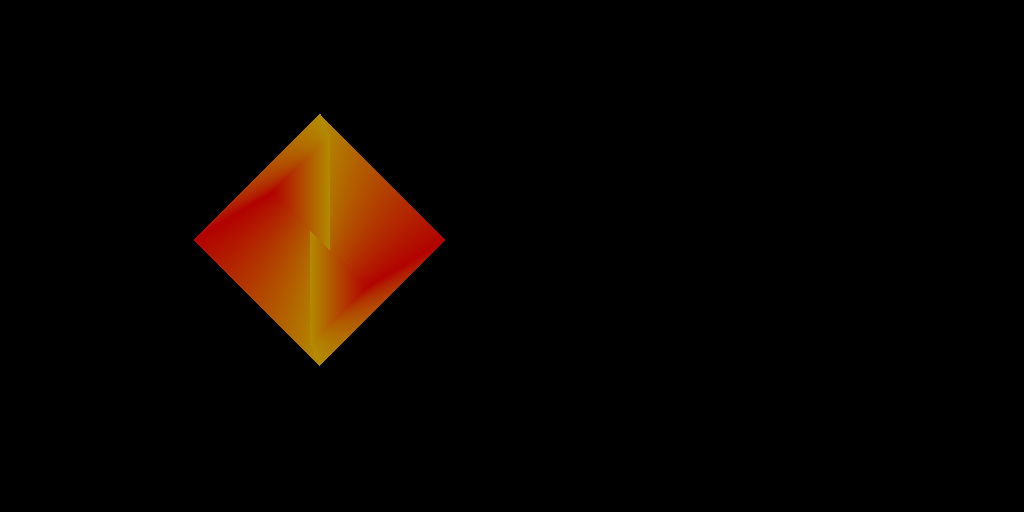
\includegraphics[width=\textwidth]{images/first-triangles}
  \caption{First output of our OpenGL renderer}
  \label{fig:renderer_first_triangles}
\end{figure}

We should now finally be ready to draw ou first triangles. If you
restart the emulator you should end up with the image in
figure~\ref{fig:renderer_first_triangles}.

The two triangles start back-to-back and then move and shrink to their
final position. Since we don't yet draw the background quad they're
all drawn on top of each other which gives this color smearing
effect. Note that the image has a weird aspect ratio (2:1) and that
the logo is not centered, it's because we're displaying the entire
VRAM framebuffer instead of just the 640x480 portion configured in the
video output.

\subsection{OpenGL debugging}

You might have noticed that there's not a whole lot of error checking
in my OpenGL code above. We could call `GetError` after every OpenGL
function but that's annoying an noisy. Instead I prefer to use the
\href{https://www.khronos.org/registry/gles/extensions/KHR/debug.txt}{debug
  extension}.

This extension logs errors, warnings, performance notices and other
messages to an internal queue. We can then call
\code{GetDebugMessageLog} to retreive the messages\footnote{I'm
  leaving out the definition of the various \code{Debug*} types which
  are just thin wrappers around the OpenGL values, as always check the
  repository if you want to see the entire code.}:

\begin{lstlisting}
/// Check for OpenGL errors using `gl::GetDebugMessageLog`. If a
/// severe error is encountered this function panics. If the OpenGL
/// context doesn't have the DEBUG attribute this *probably* won't do
/// anything.
pub fn check_for_errors() {
    let mut fatal = false;

    loop {
        let mut buffer = vec![0; 4096];

        let mut severity = 0;
        let mut source = 0;
        let mut message_size= 0;
        let mut mtype = 0;
        let mut id = 0;

        let count =
            unsafe {
                gl::GetDebugMessageLog(1,
                                       buffer.len() as GLsizei,
                                       &mut source,
                                       &mut mtype,
                                       &mut id,
                                       &mut severity,
                                       &mut message_size,
                                       buffer.as_mut_ptr() as *mut GLchar)
            };

        if count == 0 {
            // No messages left
            break;
        }

        buffer.truncate(message_size as usize);

        let message =
            match str::from_utf8(&buffer) {
                Ok(m) => m,
                Err(e) => panic!("Got invalid message: {}", e),
            };

        let source = DebugSource::from_raw(source);
        let severity = DebugSeverity::from_raw(severity);
        let mtype = DebugType::from_raw(mtype);

        println!("OpenGL [{:?}|{:?}|{:?}|0x{:x}] {}",
                 severity, source, mtype, id, message);

        if severity.is_fatal() {
            // Something is very wrong, don't die just yet in order to
            // display any additional error message
            fatal = true;
        }
    }

    if fatal {
        panic!("Fatal OpenGL error");
    }
}
\end{lstlisting}

We can then call the \code{check\_for\_errors} method after critical
sections: in `draw` for instance to check for errors in the past frame
but also at the end of `new` to make sure the initialization went
well. There's one caveat though: the debug extension only works when
we use a debug OpenGL context. We can get one by setting the
\code{CONTEXT\_DEBUG} attribute before we create the window:

\begin{lstlisting}
sdl2::video::gl_set_attribute(
                    GLAttr::GLContextFlags,
                    sdl2::video::GL_CONTEXT_DEBUG.bits());
\end{lstlisting}

A debug context might be slower than a normal one though so we'll
probably want to only activate this for troubleshooting (via a command
line flag or something like that). For now performances don't matter
in the least so we can leave it enabled at all times.

The error messages themselves are vendor specific but hopefully they
should be helpful. For instance with my radeon card if I mess up my
vertex shader by replacing \code{vec3} by \code{vec4} in the color
affectation I get the following message:

\begin{verbatim}
OpenGL [High|ShaderCompiler|Error|0x1] 0:19(10):
error: too few components to vec4
\end{verbatim}

\subsection{Drawing quadrilaterals}

Modern OpenGL doesn't support quads, only points, lines and
triangles\footnote{Although you can emulate proper quad shading in
  shaders if you really need to.}. Fortunately for us, neither does
the Playstation GPU! When a quad draw command is received it's
interpreted as two triangles and drawn that way. This is significant
for gouraud shaded quadrilaterals since it means that only three
vertices are ever used to interpolate the color of any pixel in the
quad. For textured quads it shouldn't make any difference.

We can emulate that behavior in a \code{push\_quad} method:

\begin{lstlisting}
Impl Renderer {
    //...

    /// Add a quad to the draw buffer
    pub fn push_quad(&mut self,
                     positions: [Position; 4],
                     colors:    [Color; 4]) {

        // Make sure we have enough room left to queue the vertex. We
        // need to push two triangles to draw a quad, so 6 vertex
        if self.nvertices + 6 > VERTEX_BUFFER_LEN {
            // The vertex attribute buffers are full, force an early
            // draw
            self.draw();
        }

        // Push the first triangle
        for i in 0..3 {
            self.positions.set(self.nvertices, positions[i]);
            self.colors.set(self.nvertices, colors[i]);
            self.nvertices += 1;
        }

        // Push the 2nd triangle
        for i in 1..4 {
            self.positions.set(self.nvertices, positions[i]);
            self.colors.set(self.nvertices, colors[i]);
            self.nvertices += 1;
        }
    }
}
\end{lstlisting}

We must duplicate the two vertices shared by the two triangles across
one of the quad's diagonal so we end up with 6 vertices for a single
quad. It's possible to avoid that duplication (for instance by using
indexed rendering) but at that point it would be premature
optimization.

Now all that's left to do is to is use \code{push\_quad} to draw the
monochrome and shaded quadrilaterals:

\begin{lstlisting}
impl Gpu {
    //...

    /// GP0(0x28): Monochrome Opaque Quadrilateral
    fn gp0_quad_mono_opaque(&mut self) {
        let positions = [
            Position::from_gp0(self.gp0_command[1]),
            Position::from_gp0(self.gp0_command[2]),
            Position::from_gp0(self.gp0_command[3]),
            Position::from_gp0(self.gp0_command[4]),
            ];

        // Only one color repeated 4 times
        let colors = [ Color::from_gp0(self.gp0_command[0]); 4];

        self.renderer.push_quad(positions, colors);
    }

   /// GP0(0x38): Shaded Opaque Quadrilateral
    fn gp0_quad_shaded_opaque(&mut self) {
        let positions = [
            Position::from_gp0(self.gp0_command[1]),
            Position::from_gp0(self.gp0_command[3]),
            Position::from_gp0(self.gp0_command[5]),
            Position::from_gp0(self.gp0_command[7]),
            ];

        let colors = [
            Color::from_gp0(self.gp0_command[0]),
            Color::from_gp0(self.gp0_command[2]),
            Color::from_gp0(self.gp0_command[4]),
            Color::from_gp0(self.gp0_command[6]),
            ];

        self.renderer.push_quad(positions, colors);
    }
}
\end{lstlisting}

Even though we use per-vertex colors it's easy to draw monochrome
primitives by repeating the same color. We have encountered a third
quad command, \code{gp0\_quad\_texture\_blend\_opaque} but since we
don't support textures we can't implement that correctly yet. In the
meantime we can use a solid color instead, it won't look right but at
least we'll see \emph{something}:

\begin{lstlisting}
impl Gpu {
    //...

    /// GP0(0x2C): Textured Opaque Quadrilateral
    fn gp0_quad_texture_blend_opaque(&mut self) {
        let positions = [
            Position::from_gp0(self.gp0_command[1]),
            Position::from_gp0(self.gp0_command[3]),
            Position::from_gp0(self.gp0_command[5]),
            Position::from_gp0(self.gp0_command[7]),
            ];

        // XXX We don't support textures for now, use a solid red
        // color instead
        let colors = [ Color(0x80, 0x00, 0x00); 4];

        self.renderer.push_quad(positions, colors);
    }
}
\end{lstlisting}

\begin{figure}[ht]
  \centering
  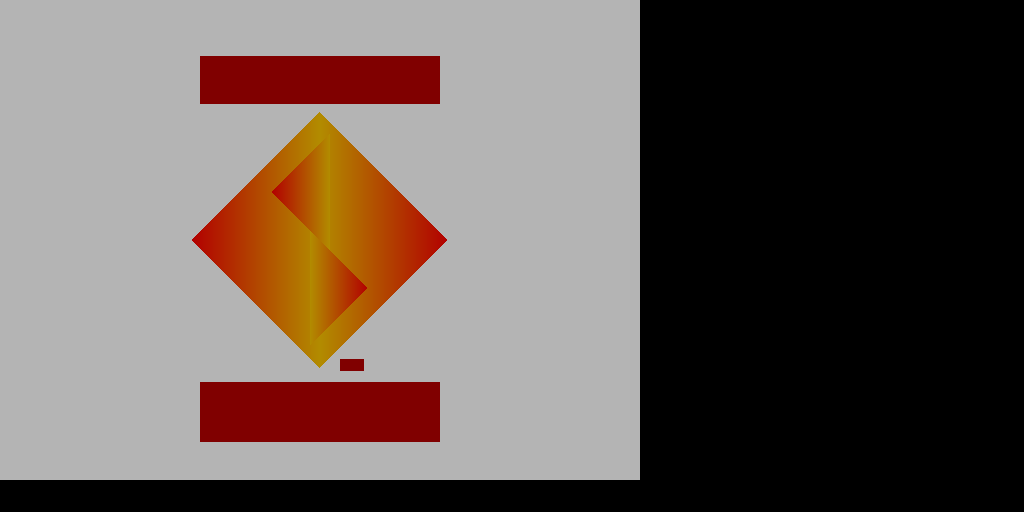
\includegraphics[width=\textwidth]{images/logo-notextures}
  \caption{Playstation boot logo without textures}
  \label{fig:bootlogo_notextures}
\end{figure}

Lo and behold, we should now have something that looks very much like the
``Sony Computer Entertainment'' boot logo, minus the text which is
contained in the textures. Figure~\ref{fig:bootlogo_notextures} shows
the expected output.

\begin{figure}[ht]
  \centering
  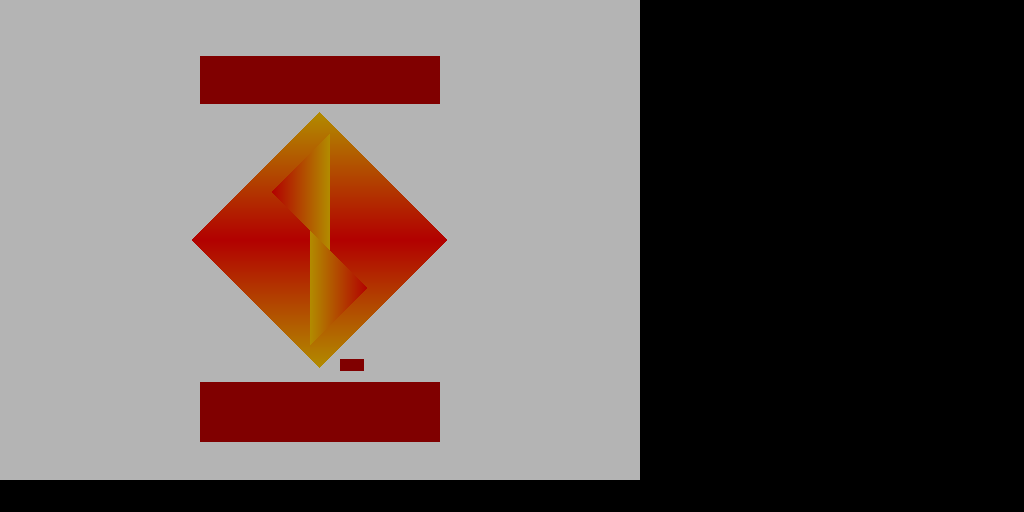
\includegraphics[width=\textwidth]{images/logo-badquad}
  \caption{Playstation boot logo with bad quad rendering}
  \label{fig:bootlogo_badquad}
\end{figure}

As before the black area at the right and bottom of the image is due
to the fact that we display the entire framebuffer instead of just the
part configured in the video output. You can see that a single 640x480
image already takes more than half of the entire VRAM and we're only
displaying a very simple logo. Game developers back then had to be
very careful with VRAM usage (and memory usage in general). This is
also one of the reasons most games are rendered at lower resolutions
like 640x240, but we'll see that later.

Note that there are two ways to split a quadrilateral in two triangles
by cutting along either diagonal. The choice is significant,
figure~\ref{fig:bootlogo_badquad} shows the result of splitting across
the other diagonal\footnote{I modified \code{push\_quad}: instead of
  rendering triangles with vertex indexes [0,~1,~2] and [1,~2,~3] I
  used [2,~3,~0] and [3,~0,~1].}. You can see that the main ``tilted
square'' behind the two triangles is shaded differently. If your
emulator's output looks like this it means that you're not rendering
the quads in the right order, you need to split along the other
diagonal.

\subsection{Draw Offset emulation}

Our OpenGL renderer is very basic but we can at least add the draw
offset easily. Of course the most obvious way would be to add it to
the \code{Position}s before we put them in the attribute buffer but
instead we can have the vertex shader do it for us!

In order to do this we can declare an ``uniform'' in the shader code:

\begin{lstlisting}[language=glsl]
//...

// Drawing offset
uniform ivec2 offset;

void main() {
  ivec2 position = vertex_position + offset;

  // Convert VRAM coordinates (0;1023, 0;511) into
  // OpenGL coordinates (-1;1, -1;1)
  float xpos = (float(position.x) / 512) - 1.0;
  // VRAM puts 0 at the top, OpenGL at the bottom,
  // we must mirror vertically
  float ypos = 1.0 - (float(position.y) / 256);

  gl_Position.xyzw = vec4(xpos, ypos, 0.0, 1.0);

  //...
}
\end{lstlisting}

Uniforms are inputs that are shared across all the intances of the
shader. So instead of having an \code{offset} vertex attribute with
one entry per vertex we can have a single variable that will be used
for an entire batch of primitives.

To be able to modify the value of the uniform from our code we must
retreive the index like we did for the vertex attributes. We can then
set its value using \code{Uniform2i}\footnote{The \code{2i} part means
  that the function works on \code{ivec2}s, there are other
  \code{Uniform*} functions for the various other types.}:

\begin{lstlisting}
impl Renderer {
    //...

    /// Index of the "offset" shader uniform
    uniform_offset: GLint,
}

impl Renderer {

    pub fn new() -> Renderer {
        //...

        // Retreive and initialize the draw offset
        let uniform_offset = find_program_uniform(program,
                                                 "offset");
        unsafe {
            gl::Uniform2i(uniform_offset, 0, 0);
        }

        Renderer {
            //...

            uniform_offset: uniform_offset,
        }
    }

    //...
}
\end{lstlisting}

We can now add a method to set the value of the uniform. We need to be
careful to draw the currently buffered primitives before we change the
offset since those were supposed to be drawn with the previous value
and might end up located at the wrong place:

\begin{lstlisting}
impl Renderer {
    //...

    /// Set the value of the uniform draw offset
    pub fn set_draw_offset(&mut self, x: i16, y: i16) {
        // Force draw for the primitives with the current offset
        self.draw();

        // Update the uniform value
        unsafe {
            gl::Uniform2i(self.uniform_offset,
                          x as GLint,
                          y as GLint);
        }
    }
}
\end{lstlisting}

Finally we can get rid of our \code{drawing\_x\_offset} and
\code{drawing\_y\_offset} member variables in the GPU and call
\code{set\_draw\_offset} directly instead.

The fact that we have to force a partial draw every time the offset is
changed means that in pathological cases this might end up being
slower. For instance if a game draws thounsands of triangles, changing
the offset between each one, we'll issue thousands of partial draw
commands. In this case it would probably be faster to simply add the
offset before we push the \code{Position}s in the attribute buffer.

\subsection{Handling SDL2 events and exiting cleanly}

Before we move on I want to fix one annoying problem introduced by our
brand new SDL2 window: since we don't handle SDL events we can't exit
the emulator cleanly. And since SDL2 catches SIGINT by default we
can't even interrupt our emulator with \verb|^C| anymore.

Fortunately it's an easy fix: instead of initializing the SDL context
in the \code{Renderer} we move it all the way up in the \code{main}
function and then check for events in the top level loop. Since we
need the SDL context to create the window we also have to shuffle
constructors a bit: I've decided to create the renderer in the main
function then move it into the \code{Gpu} constructor which is itself
moved into the \code{Interconnect} constructor:

\begin{lstlisting}
use sdl2::event::Event;
use sdl2::keycode::KeyCode;

fn main() {
    let bios = Bios::new(&Path::new("roms/SCPH1001.BIN")).unwrap();

    // We must initialize SDL before the interconnect is created since
    // it contains the GPU and the GPU needs to create a window
    let sdl_context = sdl2::init(::sdl2::INIT_VIDEO).unwrap();

    let renderer = Renderer::new(&sdl_context);
    let gpu = Gpu::new(renderer);
    let inter = Interconnect::new(bios, gpu);
    let mut cpu = Cpu::new(inter);

    let mut event_pump = sdl_context.event_pump();

    loop {
        for _ in 0..1_000_000 {
            cpu.run_next_instruction();
        }

        // See if we should quit
        for e in event_pump.poll_iter() {
            match e {
                Event::KeyDown { keycode: KeyCode::Escape, .. } => return,
                Event::Quit {..} => return,
                _ => (),
            }
        }
    }
}
\end{lstlisting}

When the \code{Quit} event is encountered (window closes, received
SIGINT etc...) we return from main, effectively exiting the
program. For convenience I also quit when the \code{Escape} key is
pressed in the window.

The inner \code{for} loop is needed because checking for events before
every instruction slows everything down very significantly so I only
check once for every million instruction executed.

\section{The Interconnect: Generic loads and stores}

At this point we have three load and three store methods in our
interconnect to deal with byte, halfword and word accesses. Those
implementations look very similar to each other.

When we implement the debugger and the timings you'll see that we'll
need special versions of those methods. At this rate we'll end up with
dozens of memory access functions that will be very similar but for a
few key differences.

This is a lot of potential code duplication. Fortunately we can avoid
most of it by making our code use generics instead of having different
flavors for 8, 16 and 32bit loads and store.

The first step is to create a generic \code{Addressable} trait:

\begin{lstlisting}
/// Types of access supported by the Playstation architecture
#[derive(PartialEq,Eq,Debug)]
pub enum AccessWidth {
    Byte = 1,
    Halfword = 2,
    Word = 4,
}

/// Trait representing the attributes of a primitive addressable
/// memory location.
pub trait Addressable {
    /// Retreive the width of the access
    fn width() -> AccessWidth;
    /// Build an Addressable value from an u32. If the Addressable is 8
    /// or 16bits wide the MSBs are discarded to fit.
    fn from_u32(u32) -> Self;
    /// Retreive the value of the Addressable as an u32. If the
    /// Addressable is 8 or 16bits wide the MSBs are padded with 0s.
    fn as_u32(self) -> u32;
}
\end{lstlisting}

We can then implement this trait for \code{u8}, \code{u16} and
\code{u32}:

\begin{lstlisting}
impl Addressable for u8 {
    fn width() -> AccessWidth {
        AccessWidth::Byte
    }

    fn from_u32(v: u32) -> u8 {
        v as u8
    }

    fn as_u32(&self) -> u32 {
        *self as u32
    }
}

impl Addressable for u16 {
    fn width() -> AccessWidth {
        AccessWidth::Halfword
    }

    fn from_u32(v: u32) -> u16 {
        v as u16
    }

    fn as_u32(&self) -> u32 {
        *self as u32
    }
}

impl Addressable for u32 {
    fn width() -> AccessWidth {
        AccessWidth::Word
    }

    fn from_u32(v: u32) -> u32 {
        v
    }

    fn as_u32(&self) -> u32 {
        *self
    }
}
\end{lstlisting}

\subsection{Porting the CPU code}

We can now factor our various memory access functions by making them
generic over this \code{Addressable} trait. On the CPU it looks like
this:

\begin{lstlisting}
impl Cpu {
    //...    

    /// Memory read
    fn load<T: Addressable>(&self, addr: u32) -> T {
        self.inter.load(addr)
    }
    
    /// Memory write
    fn store<T: Addressable>(&mut self, addr: u32, val: T) {
        if self.sr & 0x10000 != 0 {
            // Cache is isolated, ignore write
            println!("Ignoring store while cache is isolated");
            return;
        }

        self.inter.store(addr, val);
    }
}
\end{lstlisting}

We can then replace the various \code{load*} and \code{store*}
functions used in the CPU code by the generic versions. Most of the
time the compiler can't infer the type properly (since we're casting
all over the place to get the correct width and sign extension) so we
have to explicitly tell it which of \code{u8}, \code{u16} or
\code{u32} to use. For instance our LB implementation becomes:

\begin{lstlisting}
impl Cpu {
    //...    

    /// Load Byte (signed)
    fn op_lb(&mut self,
             instruction: Instruction,
             debugger: &mut Debugger) {

        let i = instruction.imm_se();
        let t = instruction.t();
        let s = instruction.s();

        let addr = self.reg(s).wrapping_add(i);

        // Cast as i8 to force sign extension
        let v = self.load::<u8>(addr, debugger) as i8;

        // Put the load in the delay slot
        self.load = (t, v as u32);
    }
}
\end{lstlisting}

\subsection{Porting the interconnect code}

Then we need to port our interconnect code to use the generic
interface. We have to merge the various load and store function in a
single generic one. First the load function:

\begin{lstlisting}
impl Interconnect {
    //...

    /// Interconnect: load value at `addr`
    pub fn load<T: Addressable>(&self, addr: u32) -> T {
        let abs_addr = map::mask_region(addr);

        if let Some(offset) = map::RAM.contains(abs_addr) {
            return self.ram.load(offset);
        }

        if let Some(offset) = map::BIOS.contains(abs_addr) {
            return self.bios.load(offset);
        }

        if let Some(offset) = map::IRQ_CONTROL.contains(abs_addr) {
            println!("IRQ control read {:x}", offset);
            return Addressable::from_u32(0);
        }

        if let Some(offset) = map::DMA.contains(abs_addr) {
            return self.dma_reg(offset);
        }

        if let Some(offset) = map::GPU.contains(abs_addr) {
            return self.gpu.load(offset);
        }

        if let Some(offset) = map::TIMERS.contains(abs_addr) {
            println!("Unhandled read from timer register {:x}",
                     offset);
            return Addressable::from_u32(0);
        }

        if let Some(_) = map::SPU.contains(abs_addr) {
            println!("Unhandled read from SPU register {:08x}",
                     abs_addr);
            return Addressable::from_u32(0);
        }

        if let Some(_) = map::EXPANSION_1.contains(abs_addr) {
            // No expansion implemented. Returns full ones when no
            // expansion is present
            return Addressable::from_u32(!0);
        }

        panic!("unhandled load at address {:08x}", addr);
    }
}
\end{lstlisting}

You can see that the \code{Addressable::from\_u32} function can be
used to return a literal value without having to know the real type
being used.

The store function is pretty straightforward:

\begin{lstlisting}
impl Interconnect {
    //...

    /// Interconnect: store `val` into `addr`
    pub fn store<T: Addressable>(&mut self, addr: u32, val: T) {

        let abs_addr = map::mask_region(addr);

        if let Some(offset) = map::RAM.contains(abs_addr) {
            return self.ram.store(offset, val);
        }

        if let Some(offset) = map::IRQ_CONTROL.contains(abs_addr) {
            println!("IRQ control: {:x} <- {:08x}", offset,
                     val.as_u32());
            return;
        }

        if let Some(offset) = map::DMA.contains(abs_addr) {
            return self.set_dma_reg(offset, val);
        }

        if let Some(offset) = map::GPU.contains(abs_addr) {
            return self.gpu.store(offset, val);
        }

        if let Some(offset) = map::TIMERS.contains(abs_addr) {
            println!("Unhandled write to timer register");
            return;
        }

        if let Some(_) = map::SPU.contains(abs_addr) {
            println!("Unhandled write to SPU register");
            return;
        }

        if let Some(_) = map::CACHE_CONTROL.contains(abs_addr) {
            println!("Unhandled write to CACHE_CONTROL");
            return;
        }

        if let Some(offset) = map::MEM_CONTROL.contains(abs_addr) {
            match offset {
                0 => // Expansion 1 base address
                    if val != 0x1f000000 {
                        panic!("Bad expansion 1 base address");
                    },
                4 => // Expansion 2 base address
                    if val != 0x1f802000 {
                        panic!("Bad expansion 2 base address");
                    },
                _ =>
              println!("Unhandled write to MEM_CONTROL register"),
            }

            return;
        }

        if let Some(_) = map::RAM_SIZE.contains(abs_addr) {
            // We ignore writes at this address
            return;
        }

        if let Some(offset) = map::EXPANSION_2.contains(abs_addr) {
            println!("Unhandled write to expansion 2 register");
            return;
        }

        panic!("unhandled store into address {:08x}: {:08x}",
               addr, val.as_u32());
    }
}
\end{lstlisting}

\subsection{Porting the RAM and BIOS}

For the RAM we need to know how many bytes must be loaded or
stored. We can use the \code{Addressable::width} method to figure it
out:

\begin{lstlisting}
impl Ram {
    //...

    /// Fetch the little endian value at `offset`
    pub fn load<T: Addressable>(&self, offset: u32) -> T {
        let offset = offset as usize;

        let mut v = 0;

        for i in 0..T::width() as usize {
            v |= (self.data[offset + i] as u32) << (i * 8)
        }

        Addressable::from_u32(v)
    }

    /// Store the 32bit little endian word `val` into `offset`
    pub fn store<T: Addressable>(&mut self, offset: u32, val: T) {
        let offset = offset as usize;

        let val = val.as_u32();

        for i in 0..T::width() as usize {
            self.data[offset + i] = (val >> (i * 8)) as u8;
        }
    }
}
\end{lstlisting}

The BIOS doesn't have a \code{store} method since it's read-only and
we can reuse the RAM's \code{load} code without any change.

This looping and bit fiddling might seem a little under-optimized but
LLVM seems to handle it well and generates code which looks almost
exactly like the previous non-generic version. And we have less code
duplication, so all is good.

\subsection{Porting the GPU code}

For the GPU I'll be a little more conservative: at this point I'm not
sure how it behaves when we don't use 32bit for register reads and
writes. For this reason I'll still just support 32bit access by
checking what kind of generic I'm using:

\begin{lstlisting}
impl Gpu {
    //...

    pub fn load<T: Addressable>(&self, offset: u32) -> T {

        if T::width() != AccessWidth::Word {
            panic!("Unhandled {:?} GPU load", T::width());
        }

        let r =
            match offset {
                0 => self.read(),
                4 => self.status(),
                _ => unreachable!(),
            };

        Addressable::from_u32(r)
    }

    pub fn store<T: Addressable>(&mut self, offset: u32, val: T) {

        if T::width() != AccessWidth::Word {
            panic!("Unhandled {:?} GPU load", T::width());
        }

        let val = val.as_u32();

        match offset {
            0 => self.gp0(val),
            4 => self.gp1(val),
            _ => unreachable!(),
        }
    }
}
\end{lstlisting}

\subsection{Porting the DMA code}

Likewise we only support 32bit access on the DMA registers so we can
modify the code to reflect that:

\begin{lstlisting}
impl Interconnect {
    //...

    /// DMA register read
    fn dma_reg<T: Addressable>(&self, offset: u32) -> T {

        if T::width() != AccessWidth::Word {
            panic!("Unhandled {:?} DMA load", T::width());
        }

        //...

        Addressable::from_u32(res)
    }

    /// DMA register write
    fn set_dma_reg<T: Addressable>(&mut self, offset: u32, val: T) {
        if T::width() != AccessWidth::Word {
            panic!("Unhandled {:?} DMA store", T::width());
        }

        let val = val.as_u32();

        //...
    }
}
\end{lstlisting}

Now our code should build and behave exactly like it did before. On my
system the performance is the performance is the same as far as I can
tell. This more generic infrastructure will show its usefulness soon
enough.

\section{The Debugger: Breakpoints and Watchpoints}

This section is of optional but having a good debugger can save us a
lot of time later on. Being able to disassemble the code, set
breakpoints or watchpoints or step through the assembly are invaluable
tools when we need to understand why some emulated game doesn't behave
properly in our emulator.

Writing a good debugger frontend can be quite some work however. For
simplicity's sake I've decided to implement the \href{XXXX}{GDB remote
  protocol} over a local TCP socket. This way I can just implement the
low level debugging code in the emulator and I use a general purpose
GDB binary targeting the MIPS architecture as a frontend. Then I can
debug Playstation code almost like any program using GDB, I can
disassemble the code, dump the data etc\dots{}. If I run code that I
build myself I can even provide it with debugging symbols and step
through functions and other high level niceties.

You might prefer to design the frontend yourself and integrate it
directly in the emulator. It's more work but you may add
Playstation-specific features more easily (GPU debugging comes to
mind). For this reason I'm just going to describe the low level
debugging interface in this guide, you'll decide what kind of frontend
you want to build on top.

\subsection{Debugger memory access}

\label{sec:debug-mem-access}

This part is easy, we already have the generic \code{load} and
\code{store} functions in our \code{Cpu} that we can use to access the
memory. We can simply pass a reference to our \code{Cpu} in the
debugger code and use that directly.

One potential issue with this approach is that loads and stores may
have unintended side-effects when used from the debugger. For instance
if we read from the GPUREAD register (when we properly implement it)
we ``pop'' a word from the read buffer and it'll become unavailable
when the real Playstation code wants to read it.

Later on when we implement the timings even reading from from regular
RAM will take a few emulated CPU cycles which will effectively
``waste'' some time for the emulated code and might result in a missed
interrupt or something similar.

Fortunately now that we have our generic load and store
implementations we'll only have to implement a specialized version of
those two functions if the side-effects become unmanageable in
debugging code. Those specialized functions could ignore regular
timings and even call specialized code in the various peripherals to
prevent any state change.

For the time being I'll just call the regular \code{load} and
\code{store} functions since we don't emulate enough side-effects to
make a significant difference anyway. That might change as me become
more accurate.

\subsection{Breakpoints}

Breakpoints are triggered when a certain instruction gets
executed. The instruction is identified by its memory address. We can
store the breakpoint addresses in a vector:

\begin{lstlisting}
pub struct Debugger {
    /// Vector containing all active breakpoint addresses
    breakpoints: Vec<u32>,
}
\end{lstlisting}

We then need a pair of function for adding a deleting a
breakpoint. It's a good idea to make sure we can't insert the same
address twice: insertions and deletions are going to be rare while the
address lookup will have to happen for every instruction so we want to
keep the list as small as possible:

\begin{lstlisting}
impl Debugger {
    /// Add a breakpoint that will trigger when the instruction at
    /// `addr` is about to be executed.
    fn add_breakpoint(&mut self, addr: u32) {
        // Make sure we're not adding the same address twice
        if !self.breakpoints.contains(&addr) {
            self.breakpoints.push(addr);
        }
    }

    /// Delete breakpoint at `addr`. Does nothing if there was no
    /// breakpoint set for this address.
    fn del_breakpoint(&mut self, addr: u32) {
        self.breakpoints.retain(|&a| a != addr);
    }
}
\end{lstlisting}

Finally we can implement the method \code{pc\_change} that will be
called before every instruction to look for a breakpoint at the
current address. Needless to say this code is in a very critical path
and must be as fast as possible:

\begin{lstlisting}
impl Debugger {
    //...

    /// Called by the CPU when it's about to execute a new
    /// instruction. This function is called before *all* CPU
    /// instructions so it needs to be as fast as possible.
    pub fn pc_change(&mut self, cpu: &mut Cpu) {
        if self.breakpoints.contains(&cpu.pc()) {
            self.debug(cpu);
        }
    }
}
\end{lstlisting}

The \code{debug} method is where the debugging frontend should be
notified that the execution stopped and wait for the user to resume
the execution.

Using a vector to store the breakpoints might seem sub-optimal since
it has linear lookup time. A tree-based collection could theoritically
work in logarithmic time. We have to consider two things however: we
want to optimize for the common case where no debugging is taking
place and no breakpoint is set and even when we're debugging we
\emph{probably} won't be using thousands of breakpoints
simultaneously.

Iterating over an empty vector should be very cheap: a simple test of
the length of the vector and we exit the loop immediately. And even
for small non-empty vectors it will probably be faster than a more
complex structure (strong cache locality, no cache thrashing, no
indirections, easy prefetching).

For these reasons I don't think it's necessary to bother using
anything more complicated than a good old vector, the constant cost
probably matters more than the linear complexity for our usage.

Finally we can plug \code{pc\_change} in our CPU:

\begin{lstlisting}
impl Cpu {
    //...

    /// Run a single CPU instruction and return
    pub fn run_next_instruction(&mut self, debugger: &mut Debugger) {
        // Synchronize the peripherals
        self.inter.sync(&mut self.tk);

        // Save the address of the current instruction to save in
        // `EPC` in case of an exception.
        self.current_pc = self.pc;

        // Debugger entrypoint: used for code breakpoints and stepping
        debugger.pc_change(self);

        //...
    }

    pub fn pc(&self) -> u32 {
        self.pc
    }
}
\end{lstlisting}

I pass the debugger object from the \code{main} function in order to
be able to start a debugging session at the press of a key:

\begin{lstlisting}
fn main() {
    //...

    let mut debugger = Debugger::new();

    let mut event_pump = sdl_context.event_pump();

    loop {
        for _ in 0..1_000_000 {
            cpu.run_next_instruction(&mut debugger);
        }

        // See if we should quit
        for e in event_pump.poll_iter() {
            match e {
                Event::KeyDown { keycode: KeyCode::Pause, .. } =>
                    debugger.debug(&mut cpu),
                Event::KeyDown { keycode: KeyCode::Escape, .. } =>
                    return,
                Event::Quit {..} => return,
                _ => (),
            }
        }
    }
}
\end{lstlisting}

In a quick benchmark this debugging code causes a small (but
noticeable) degradation of the performances. I think it'll probably
end up being well worth it. We could make the compilation of the
debugging code optional to make it possible to have faster binaries
when we don't want debugging but we never know when we might need it
anyway and having several build configurations makes the code harder
to test and could lead to code rot. The debugger could also
potentially be used for cheating in games so it might make sense to
leave it enabled even for ``end user'' builds.

\subsection{Watchpoints}

Being able to break on a specific instruction is useful but sometimes
we want to know when a certain location in memory is loaded or
modified. In order to do that we can implement read and write
watchpoints that will respectively check each load and store address
and trigger the debugger when a watched address is encountered.

As for breakpoints we'll store the watchpoint addresses in vectors:

\begin{lstlisting}
pub struct Debugger {
    /// Vector containing all active read watchpoints
    read_watchpoints: Vec<u32>,
    /// Vector containing all active write watchpoints
    write_watchpoints: Vec<u32>,
}
\end{lstlisting}

The methods for adding, removing and testing the watchpoints will
therefore look very similar to the breakpoint implementation:

\begin{lstlisting}
impl Debugger {
    //...

    /// Add a breakpoint that will trigger when the CPU attempts to
    /// read from `addr`
    fn add_read_watchpoint(&mut self, addr: u32) {
        // Make sure we're not adding the same address twice
        if !self.read_watchpoints.contains(&addr) {
            self.read_watchpoints.push(addr);
        }
    }

    /// Delete read watchpoint at `addr`. Does nothing if there was no
    /// breakpoint set for this address.
    fn del_read_watchpoint(&mut self, addr: u32) {
        self.read_watchpoints.retain(|&a| a != addr);
    }

    /// Called by the CPU when it's about to load a value from memory.
    pub fn memory_read(&mut self, cpu: &mut Cpu, addr: u32) {
        // XXX: how should we handle unaligned watchpoints? For
        // instance if we have a watchpoint on address 1 and the CPU
        // executes a `load32 at` address 0, should we break? Also,
        // should we mask the region?
        if self.read_watchpoints.contains(&addr) {
            println!("Read watchpoint triggered at 0x{:08x}", addr);
            self.debug(cpu);
        }
    }

    /// Add a breakpoint that will trigger when the CPU attempts to
    /// write to `addr`
    fn add_write_watchpoint(&mut self, addr: u32) {
        // Make sure we're not adding the same address twice
        if !self.write_watchpoints.contains(&addr) {
            self.write_watchpoints.push(addr);
        }
    }

    /// Delete write watchpoint at `addr`. Does nothing if there was no
    /// breakpoint set for this address.
    fn del_write_watchpoint(&mut self, addr: u32) {
        self.write_watchpoints.retain(|&a| a != addr);
    }

    /// Called by the CPU when it's about to load a value from memory.
    pub fn memory_write(&mut self, cpu: &mut Cpu, addr: u32) {
        // XXX: same remark as memory_read for unaligned stores
        if self.write_watchpoints.contains(&addr) {
            println!("Write watchpoint triggered at 0x{:08x}", addr);
            self.debug(cpu);
        }
    }
}
\end{lstlisting}

You can see that I put a few comments about unaligned access and
regions, I'm not entirely sure what's the right thing to do here. I
guess we'll see how we want the debugger to behave as we're using it.

Now we just have to plug the memory read and write methods in our
generic \code{load} and \code{store} functions in the CPU:

\begin{lstlisting}
impl Cpu {
    //...

    /// Memory read
    fn load<T: Addressable>(&mut self,
                            addr: u32,
                            debugger: &mut Debugger) -> T {
        debugger.memory_read(self, addr);

        self.inter.load(&mut self.tk, addr)
    }

    /// Memory write
    fn store<T: Addressable>(&mut self,
                             addr: u32,
                             val: T,
                             debugger: &mut Debugger) {
        debugger.memory_write(self, addr);

        if self.sr.cache_isolated() {
            self.cache_maintenance(addr, val);
        } else {
            self.inter.store(&mut self.tk, addr, val);
        }
    }
}
\end{lstlisting}

We've added an additional \code{debugger} parameter to these two
methods so we have to pass the debugger reference from
\code{run\_next\_instruction} to \code{decode\_and\_execute} and
finally to the various load and store methods that need to do memory
access (\code{op\_sw}, \code{op\_lw}, \code{op\_swr}, etc\dots{}).

There are two issues with this implementation however. First we
use this \code{store} method to fetch instructions but we don't want
to trigger a read watchpoint when we're loading instructions (that's
what breakpoints are for). The fix is easy, we just call the
interconnect's load method directly:

\begin{lstlisting}
impl Cpu {
    //...

    /// Run a single CPU instruction and return
    pub fn run_next_instruction(&mut self, debugger: &mut Debugger) {
        //...

        // Fetch instruction at PC
        let pc = self.current_pc;
        let instruction = Instruction(self.inter.load(pc));

        //...
    }
}
\end{lstlisting}

An other problem is that you might be using this CPU load method in
your debugger to read the memory's contents. Obviously you don't want
to recursively trigger the debugger when you use it to read some
memory location where a watchpoint happens to live. Instead we can
create an other method used for loading data for debugging
purposes\footnote{It can be used as a starting point for a
  ``side-effect free'' debugging path as I mentioned in
  section~\ref{sec:debug-mem-access}.}. I named this method
\code{examine}:

\begin{lstlisting}
impl Cpu {
    //...

    /// Debugger memory read
    pub fn examine<T: Addressable>(&mut self, addr: u32) -> T {
        self.inter.load(&mut self.tk, addr)
    }
}
\end{lstlisting}

\subsection{Code disassembly and beyond}

I didn't show any disassembler code since GDB does it for me but it
shouldn't be too difficult to implement since MIPS instructions are
fixed width. Just read the code you want to disassemble 32bits at a
time and then implement something similar to our
\code{decode\_and\_execute} method but instead of executing the
instruction you return the disassembled code in a string for instance.

If you want to be fancy and support MISP assembler pseudo-instructions
you'll have to handle certain instructions specifically, for instance
\mbox{\code{sll \$zero, \$zero, 0}} could be displayed as \code{nop}
while \mbox{\code{addu \$1, \$2, \$zero}} should be \mbox{\code{move
    \$1, \$2}}. Of course it's still correct if you keep the real
instructions instead of the assembler shorthand but it's generally
more readable if you use the later.

Later on we'll have to consider adding debugging for the GPU as well
(displaying primitives, textures, exploring linked lists etc\dots{}).

\section{The CPU: Instruction cache}

Before we move on to the GPU timings let's start by implementing the
CPU instruction cache. Without it we won't be able to emulate the CPU
speed properly since cached code gets executed much faster than
instructions that have to be fetched from RAM. The CPU also has a data
cache but it's not used as a proper cache so we can leave that for
later.

\subsection{Instruction cache lookup behavior}

The Playstation's CPU has a 4KB instruction cache that can contain up
to 1024 instructions across 256 4-instruction cachelines. The cache is
directly mapped which means that there's only one possible cacheline
for any given memory address.

Here's how it works: each cacheline contains enough room for 4
instructions plus a tag and valid bits. The tag contains the upper
20bits of the physical address being cached, it is used to make sure
we're really getting the data from the correct memory location and not
some other address that happens to alias the cacheline. Then for each
instruction in the cacheline a bit says if the entry is valid or
not. When fetching an instruction if the tag is mismatched or the
entry is not valid it'll have to be fetched from main memory,
otherwise we can directly use the cached value.

\begin{table}[ht]
  \centering
  \begin{tabular}{ c | c | c | c }
    Tag [31:12] & Cacheline [11:4] & Index [3:2] & Word alignment [1:0] \\
    \hline
    \code{0x80005} & \code{0x38} & \code{1} & 0 \\
  \end{tabular}

  \caption{Anatomy of cached address 0x80005384}
  \label{tab:cached-address}
\end{table}

Let's take a concrete example shown in
table~\ref{tab:cached-address}. Suppose the CPU wants to run code from
address \code{0x80005384}. First we need to figure out which cacheline
matches this address, for that we need to shift the address two bits
to the right (since we have 4 32bit words per cache line) and then
take the 8 LSBs (since we have 256 cachelines in total). In this case
we end up in cacheline number 56 (0x38).

Now that we have identified the cacheline we need to see if it already
contains data for the current address, after all any address ending in
\code{0x38X} will match the same cache location. In order to do that
we compare the tag stored in the line with bits [31:12] of the
instruction address, in this case \code{0x80005}. If the tag doesn't
match we consider it invalid and we have to fetch it from RAM.

If the tag is the one we're looking for however we just have to check
the valid bit for the instruction we're looking for. Bits [3:2] give
us the location in the 4-word cacheline, bits [1:0] are always 0 since
all instructions are word-aligned\footnote{Remember that we generate
  an exception if we ever end up with a misaligned PC so we can always
  assume that it's correctly aligned after that.} so in this case
we're looking for the 2nd word in the cacheline. If the valid bit is
set we can use it directly, otherwise the instruction is invalid and
we must fetch it from main RAM.

\subsection{Instruction cache fetch behavior}

When an invalid instruction is encountered (either because the line
has the wrong tag or the valid bit is not set) the Playstation cache
will will update the tag to match the current address and then fetch
the missing instruction as well as any \emph{following} instruction in
the same cacheline, but not the one before it.

For instance in the case of address \code{0x80005384} if we have a
cache miss the instructions at addresses \code{0x80005384},
\code{0x80005388} and \code{0x8000538c} will be fetched (words at
indexes 1, 2 and 3 respectively) but \emph{not} \code{0x80005380} (the
word at index 0). I suppose that if some of the following instructions
are already valid they're not fetched again but I haven't tested it
and it's probably not very common anyway.

\newpage

\listoftables
\listoffigures

\end{document}
